\documentclass{article}
\usepackage{graphicx}

\title{Tugas Database 2}
\begin{figure}
    \begin{center}
        
\includegraphics[width=6cm]{poltekpos.jpg}
    \end{center}
\end{figure}
\author{Annisa Khairani Febrianti}
\date{1184071}

\begin{document}

\maketitle
\section{Cara Membuat Aplikasi Builder Dari File Excel ke Oracle Apex}
\begin{enumerate}
    \item Buatlah data yang akan kita masukkan ke dalam Oracle APEX pada Microsoft Excel.
\begin{figure} [h]
\centerline{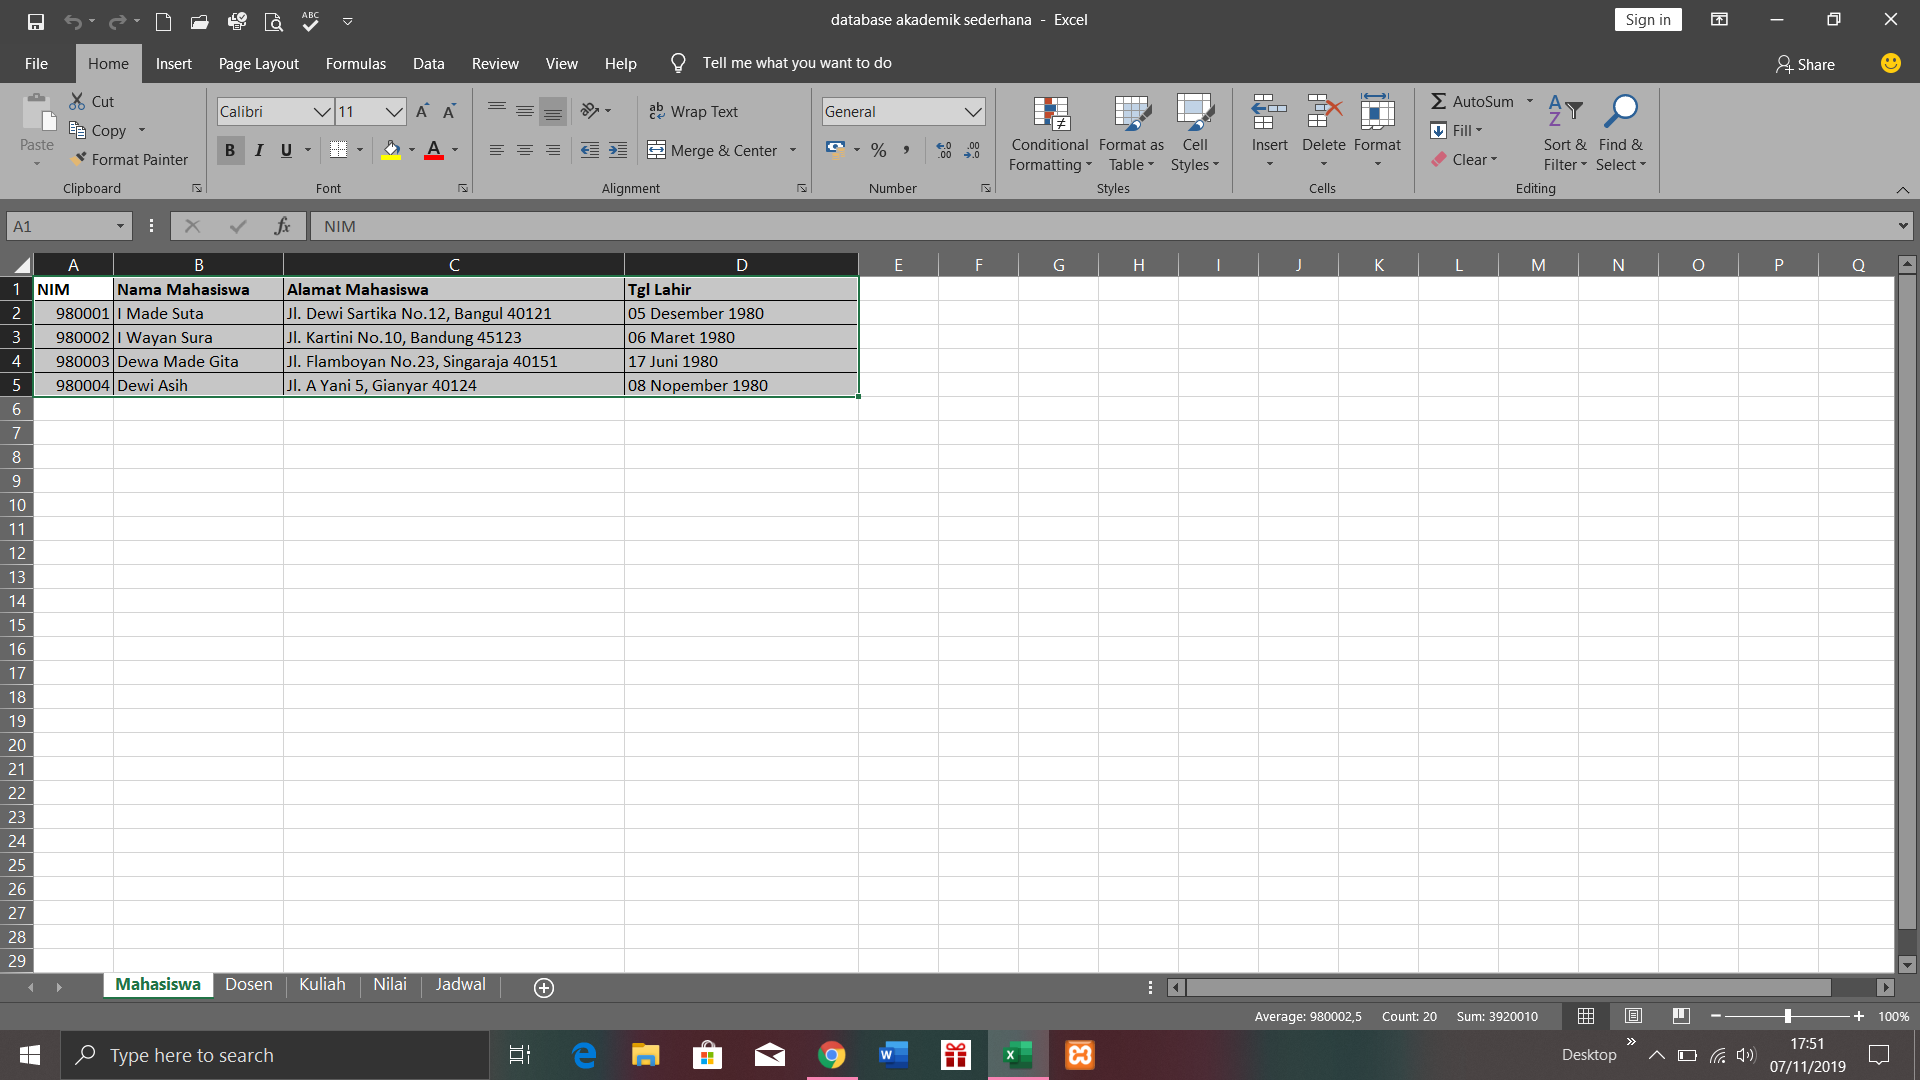
\includegraphics[width=8cm]{figure/54.png}}
\end{figure}
\newpage \begin{figure} [h]
\centerline{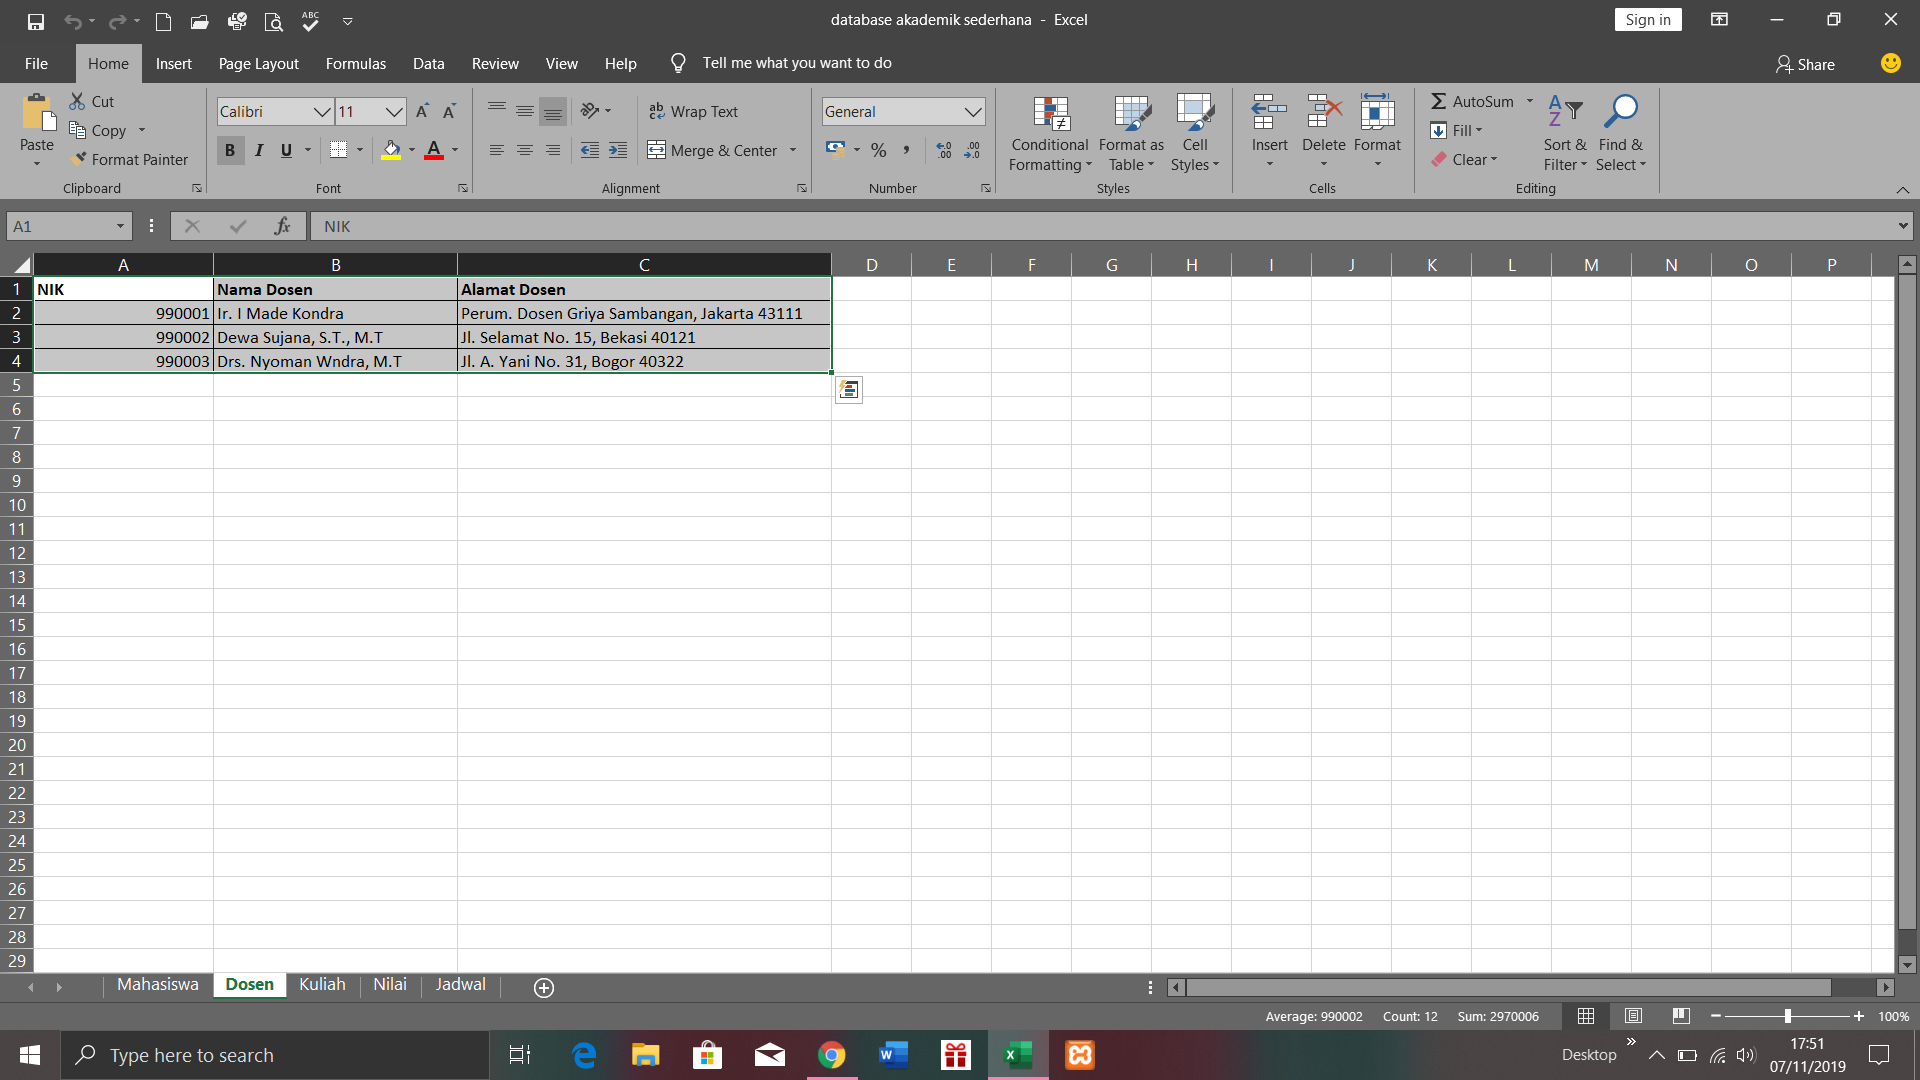
\includegraphics[width=8cm]{figure/55.png}}
\end{figure}
\begin{figure} [h]
\centerline{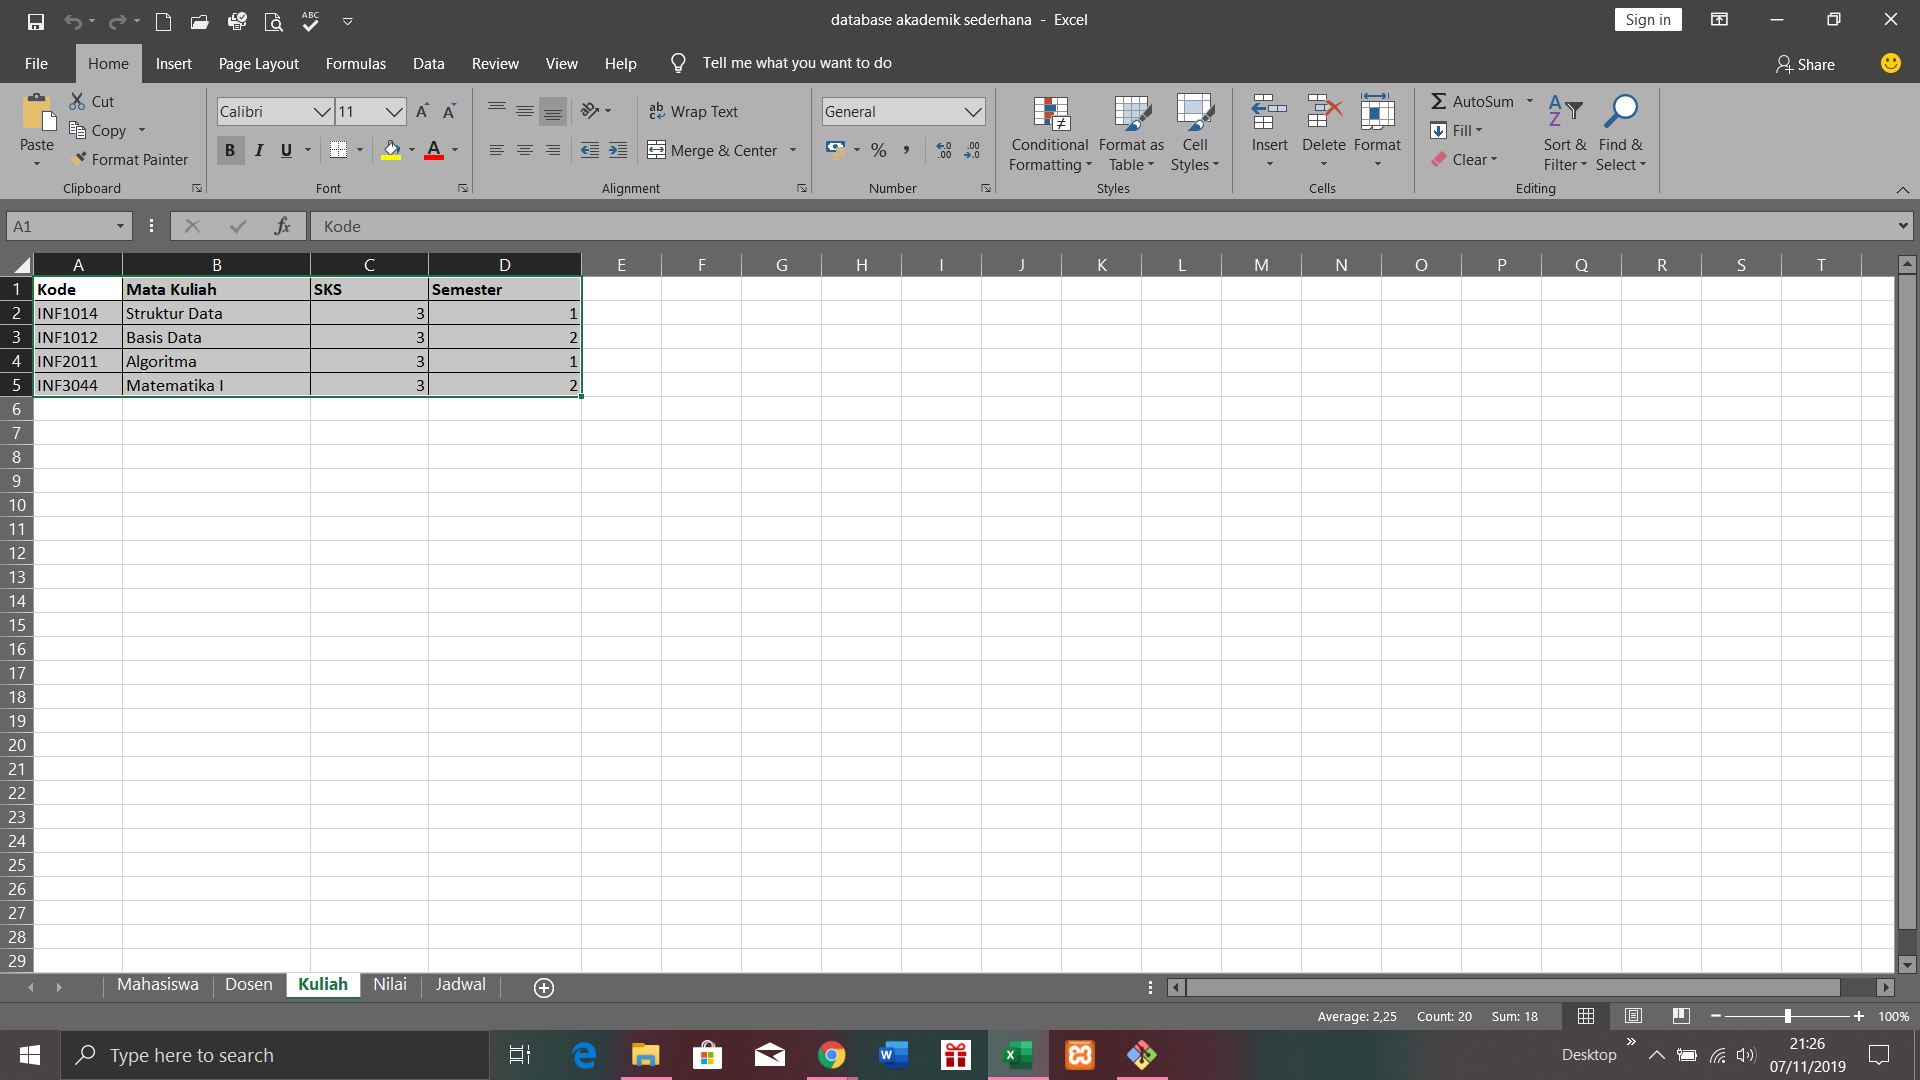
\includegraphics[width=8cm]{figure/59.png}}
\end{figure}
\begin{figure} [h]
\centerline{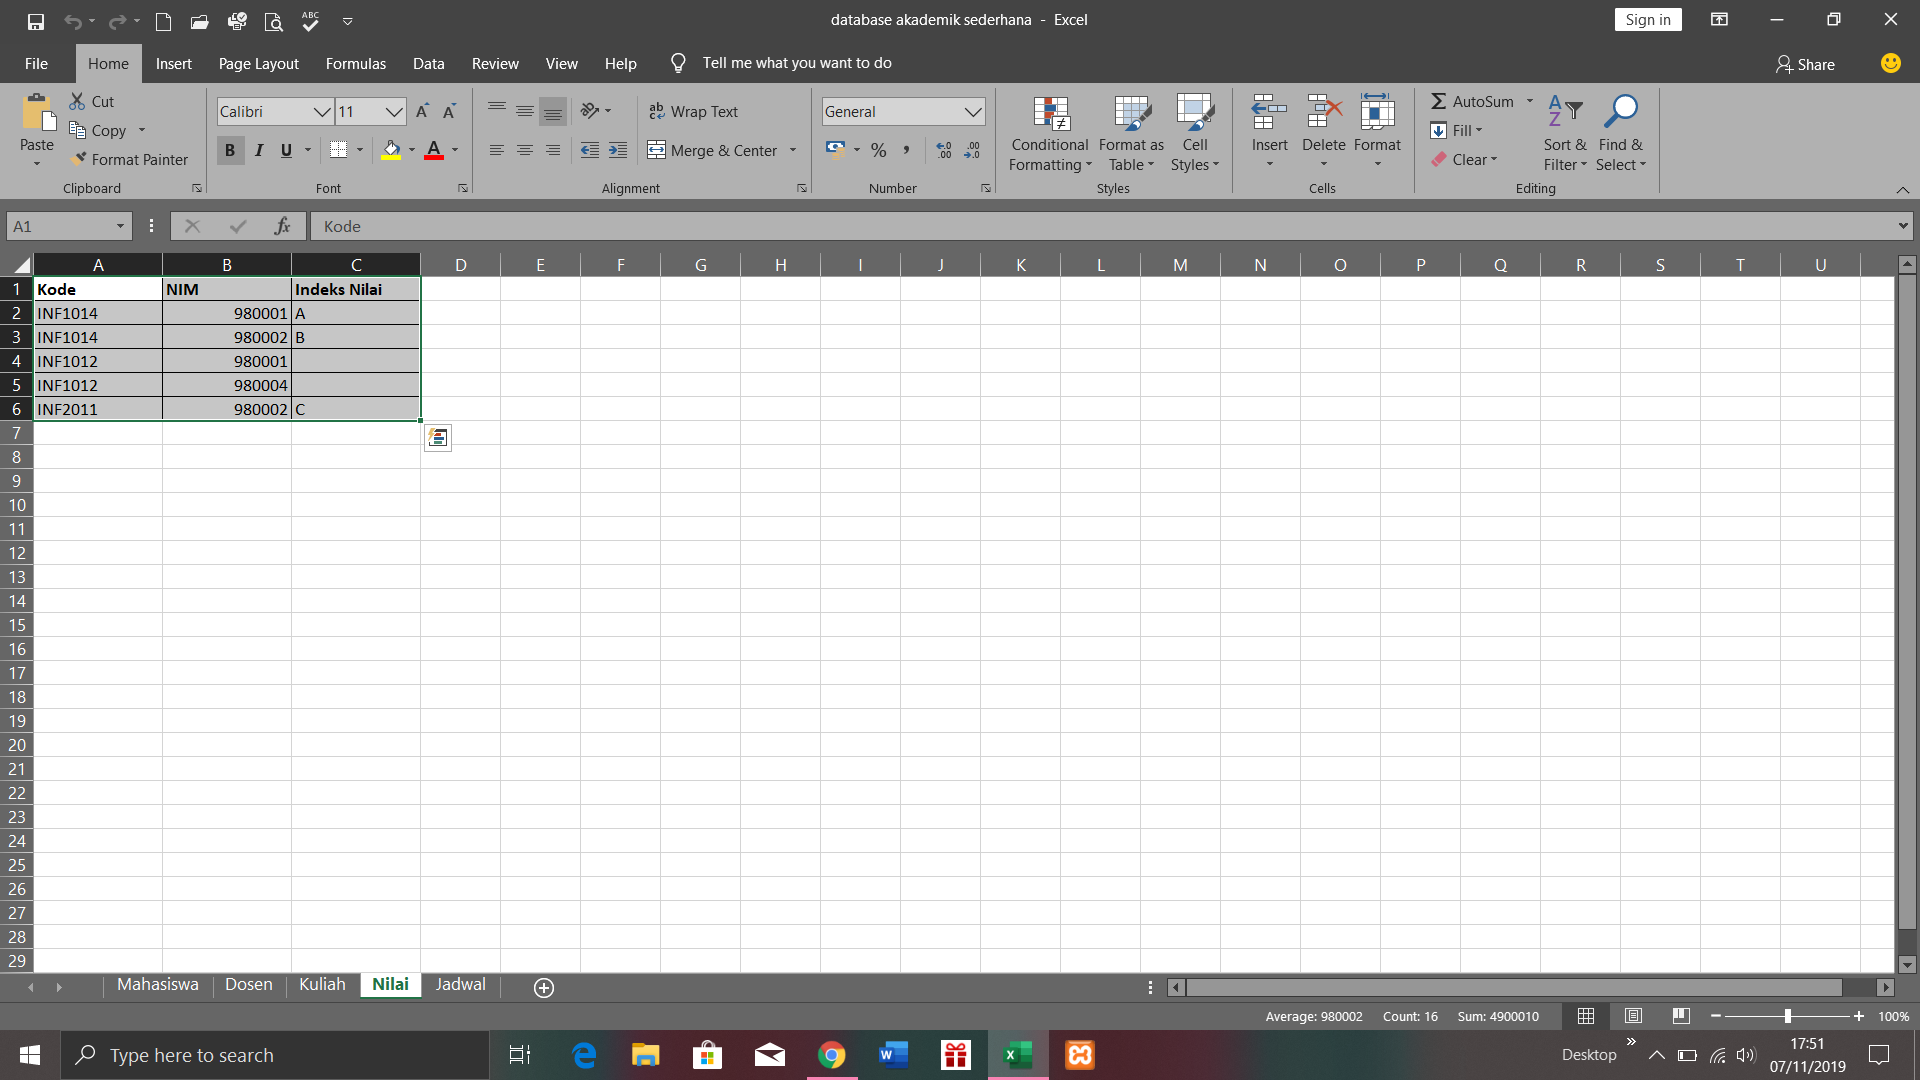
\includegraphics[width=8cm]{figure/57.png}}
\end{figure}
\begin{figure} [h]
\newpage \centerline{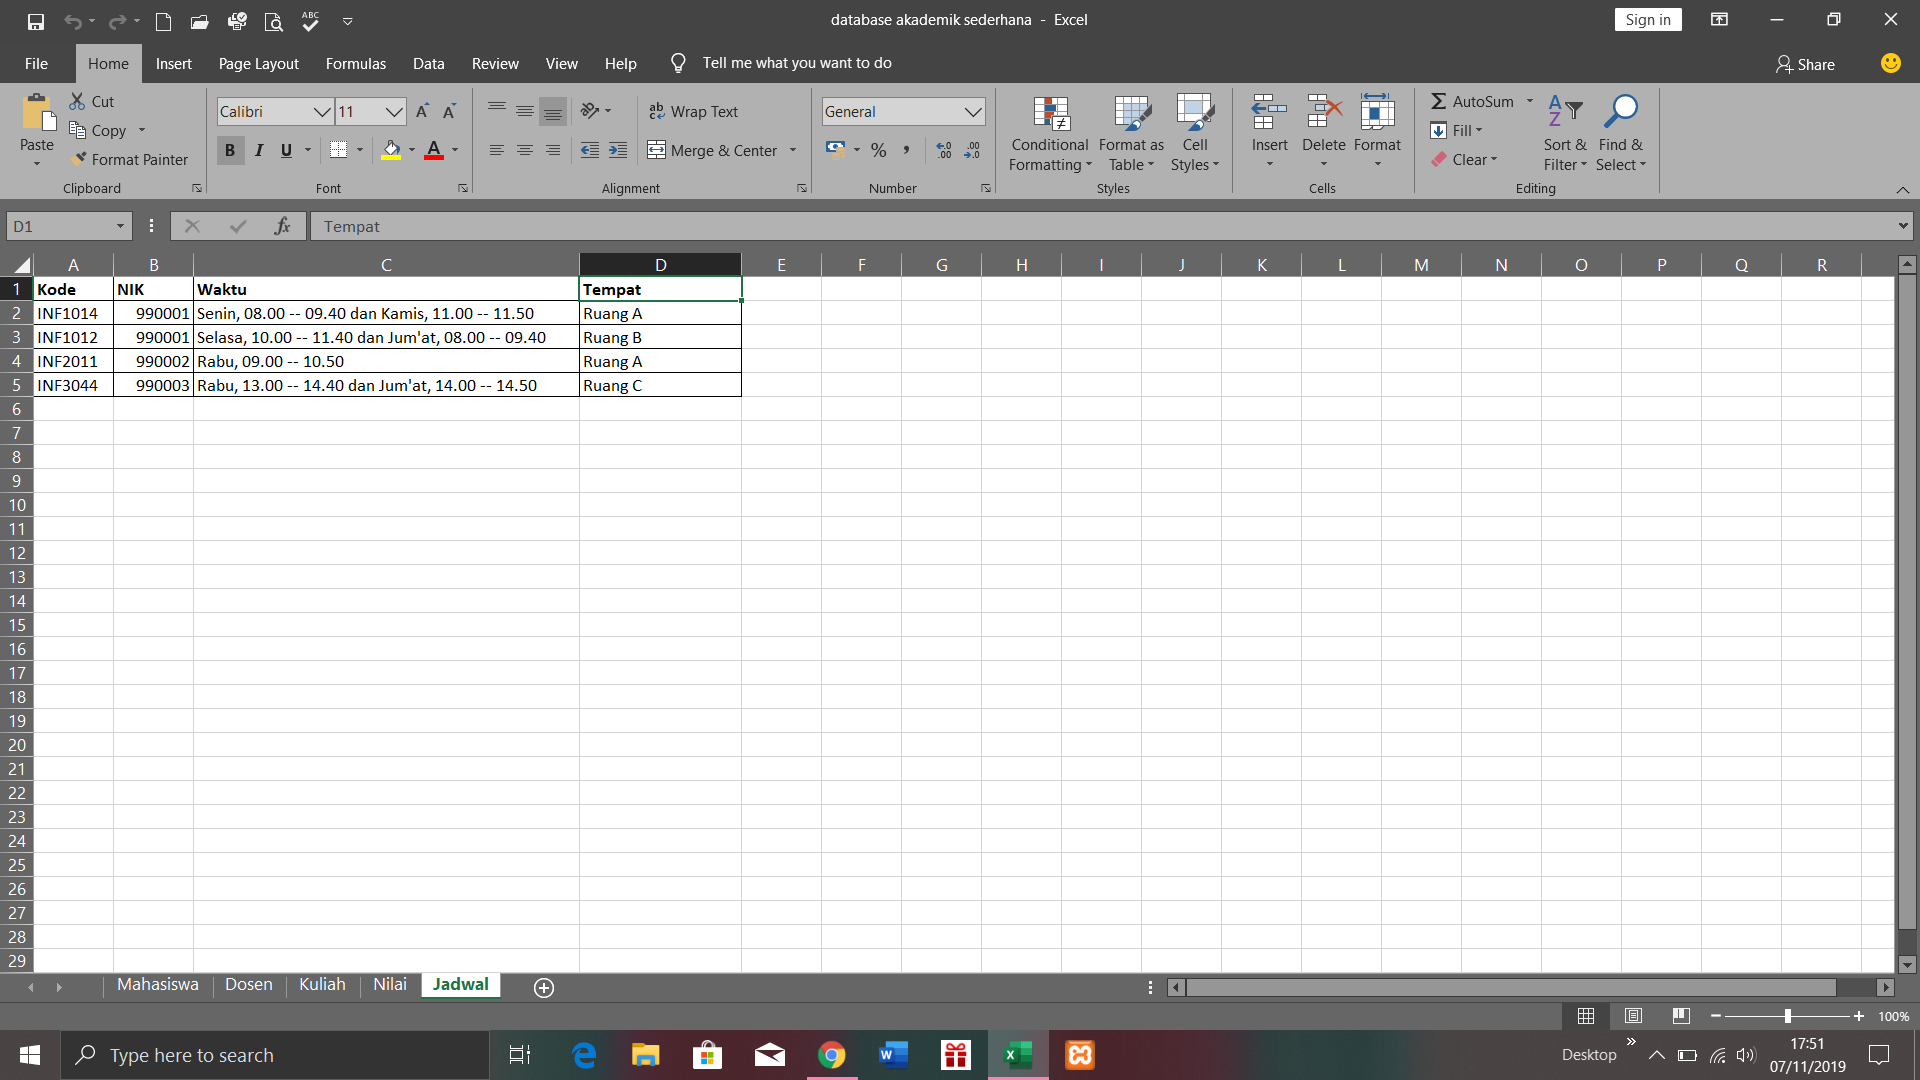
\includegraphics[width=8cm]{figure/58.png}}
\end{figure}

\newpage \par Catatan Perhatikan data yang ada pada excel karena ketika ada kesalahan dalam pembuatan data contohnya baris yang kosong tetapi masuk ke dalam data makan akan mempengaruhi data pada saat mencreate aplikasi. Dan jangan lupa untuk mernomalisasi data yang telah ada.

\section{Cara Membuat Aplikasi Builder dari File Exel ke Oracle Apex}
\begin{enumerate}
    \newpage \item Buka Oracle Apex terlebih dahulu
    \begin{figure} [h]
\newpage \centerline{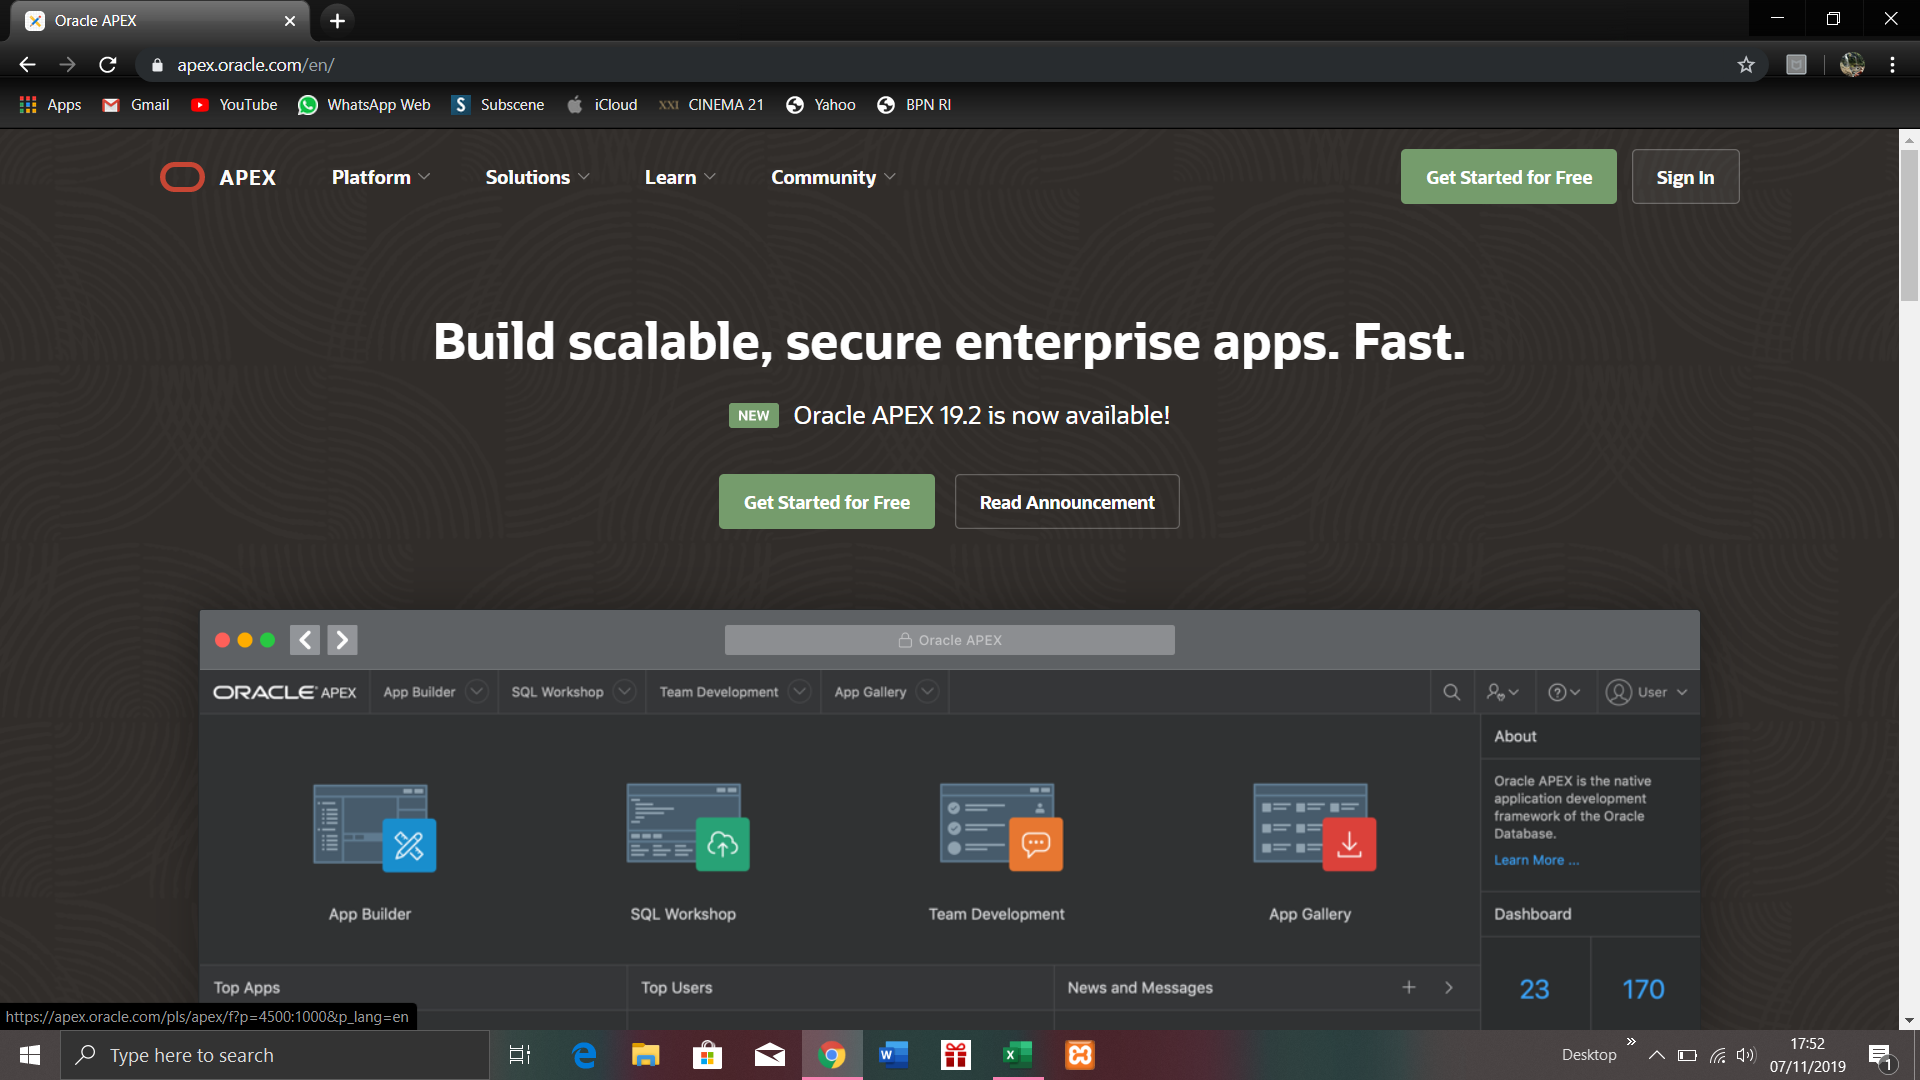
\includegraphics[width=8cm]{figure/59a.png}}
\end{figure}
    \item lalu masukkan workspace, username beserta password dan kemudian tekan sign in
    \begin{figure} [h]
\centerline{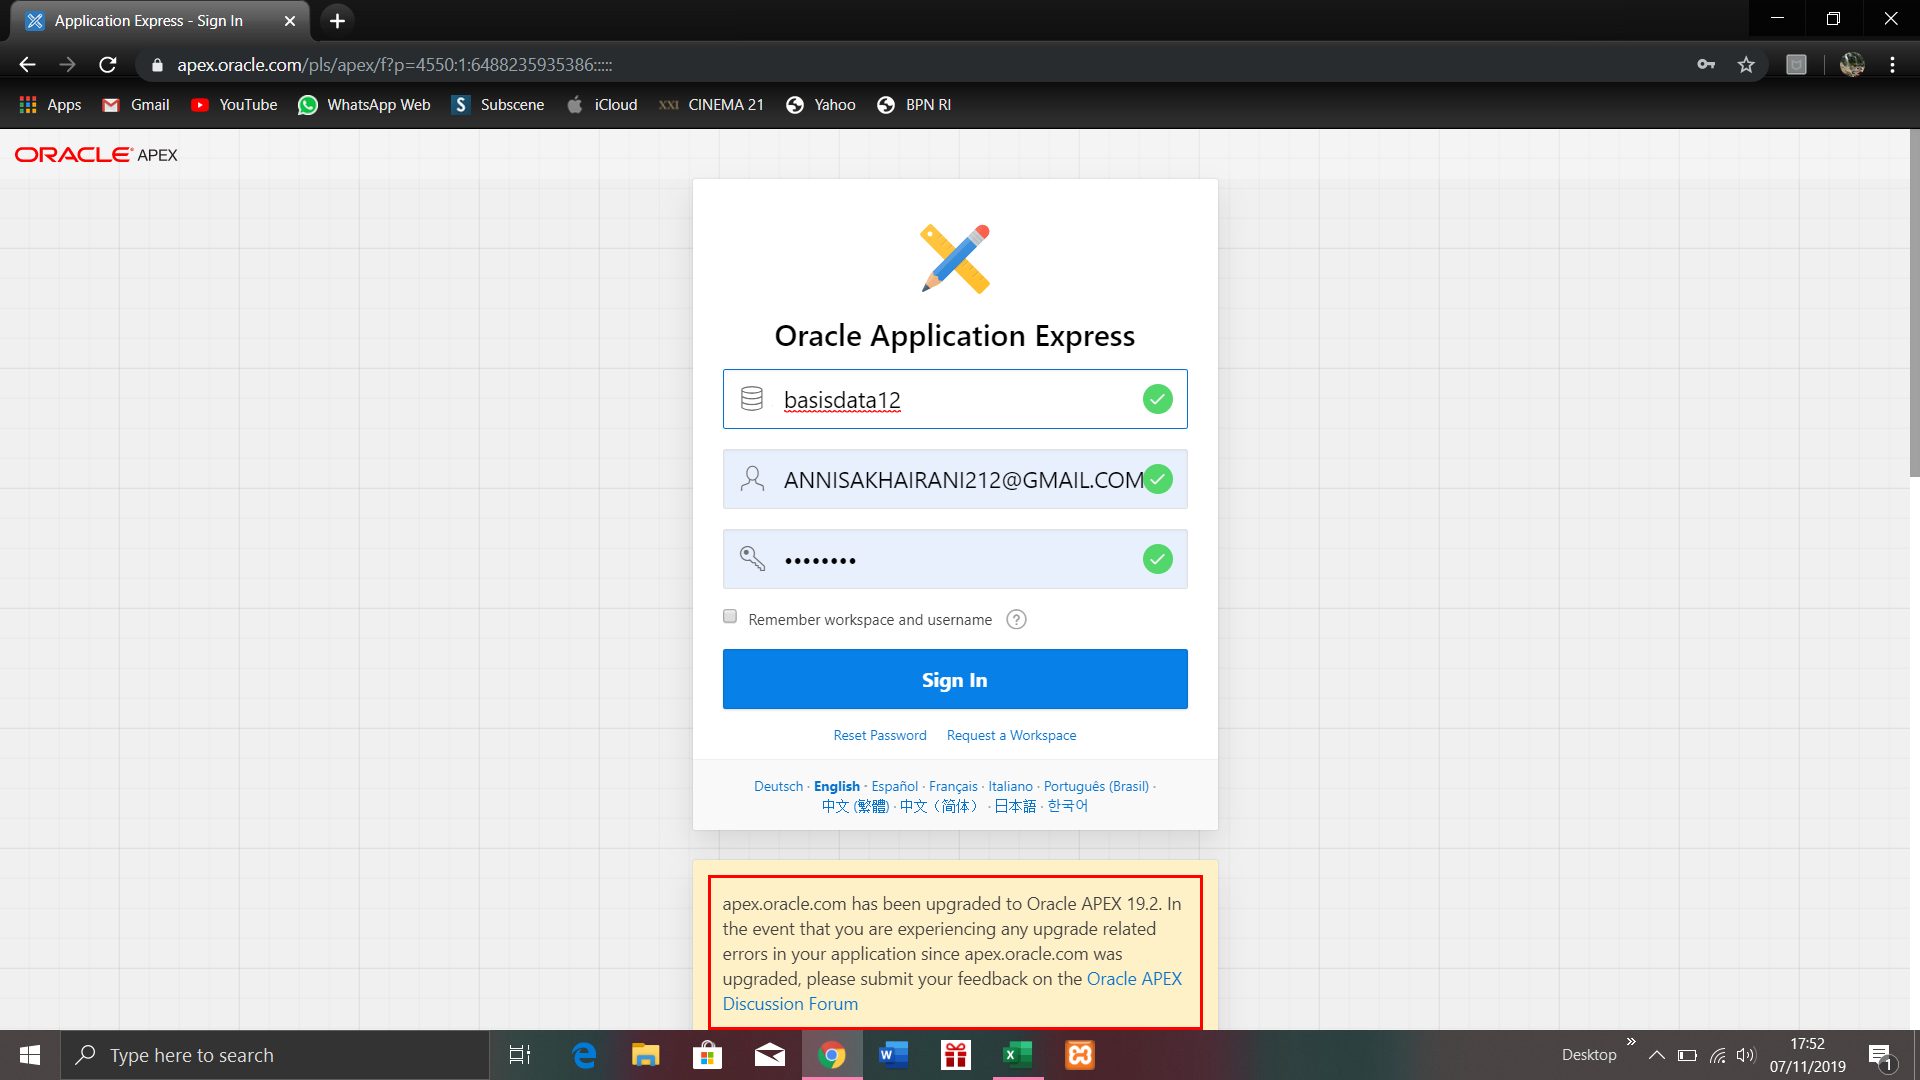
\includegraphics[width=8cm]{figure/60.png}}
\end{figure}
    \newpage \item Jika sudah masuk kemudian muncul tampilan seperti dibawah ini
    \begin{figure} [h]
\newpage \centerline{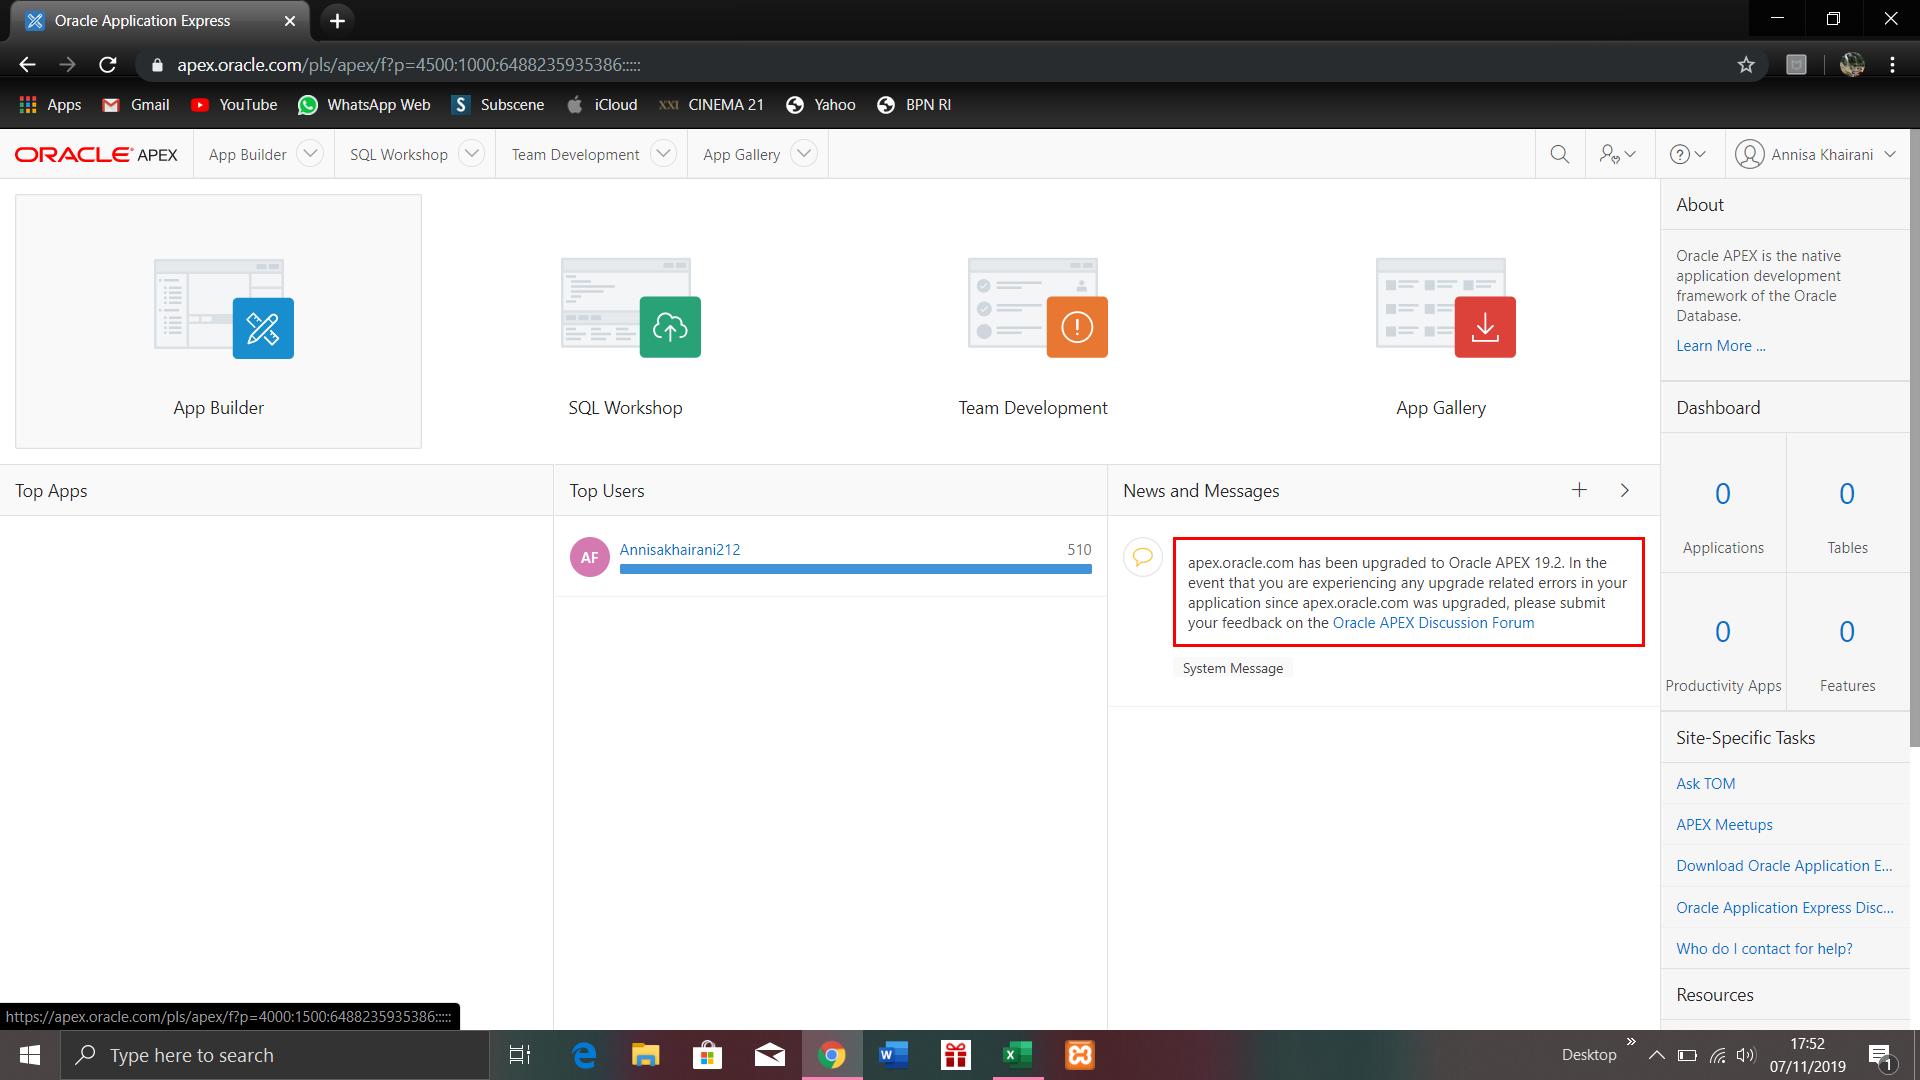
\includegraphics[width=8cm]{figure/61.png}}
\end{figure}
    \item Kemudian kita klik App Builder
    \begin{figure} [h]
\centerline{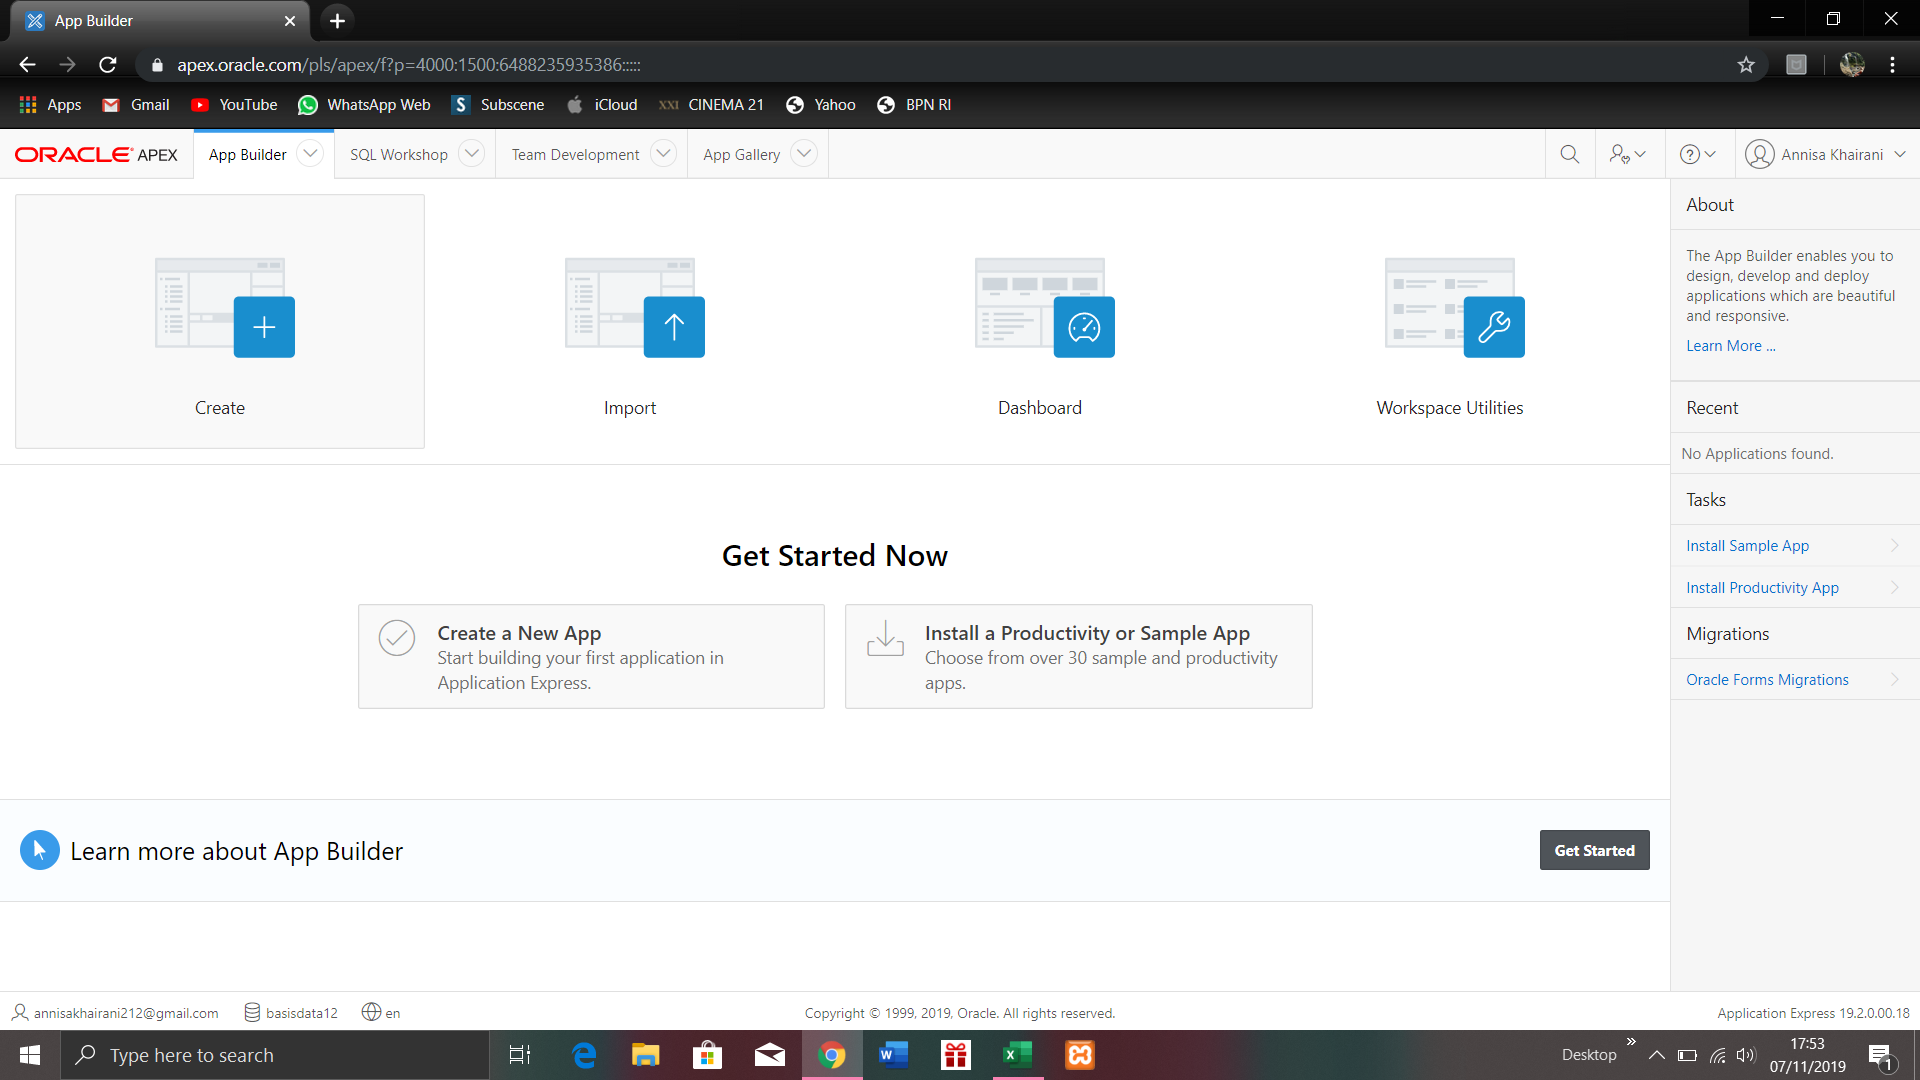
\includegraphics[width=8cm]{figure/62.png}}
\end{figure}
    \item Selanjutnya klik Creat
    \begin{center}
    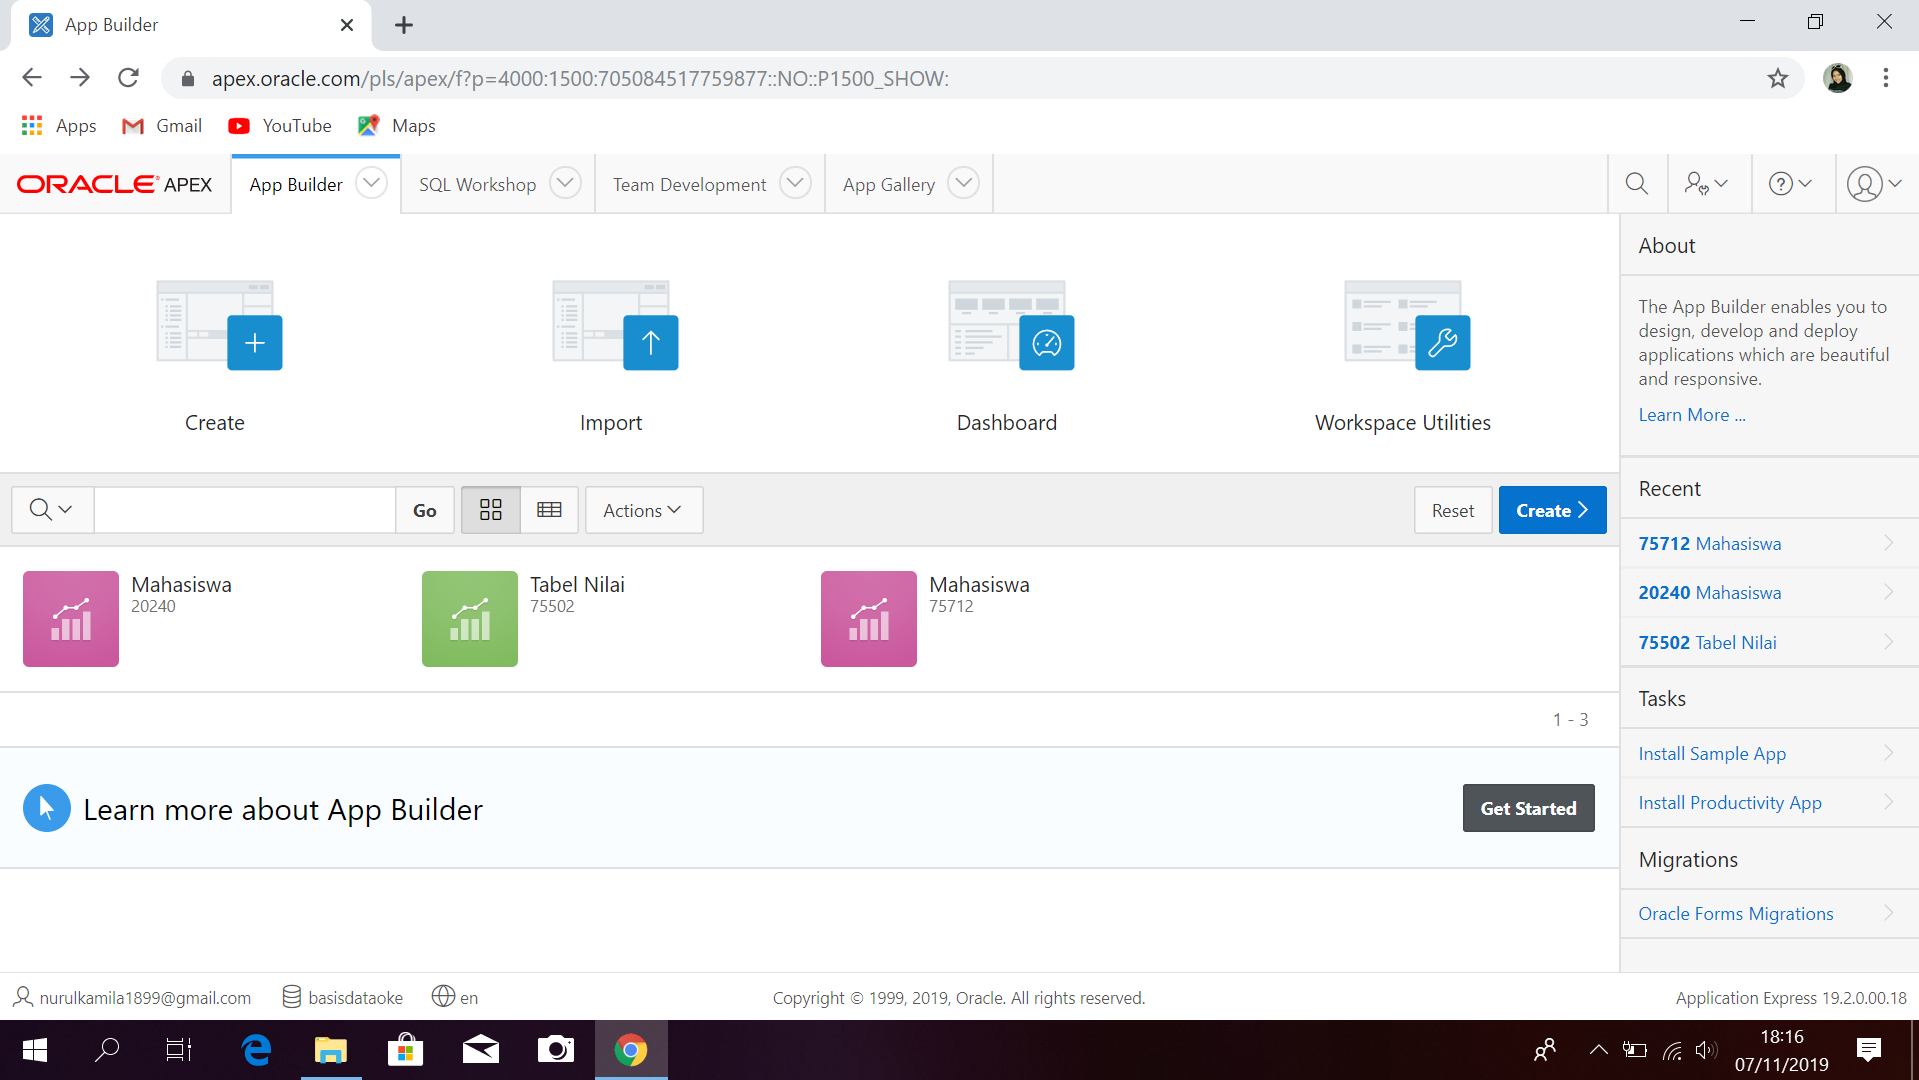
\includegraphics[width=.8\textwidth]{figure/1.PNG}
    \end{center}
    \item Pada laman Creat an Application, pilih Form a File
     \begin{center}
    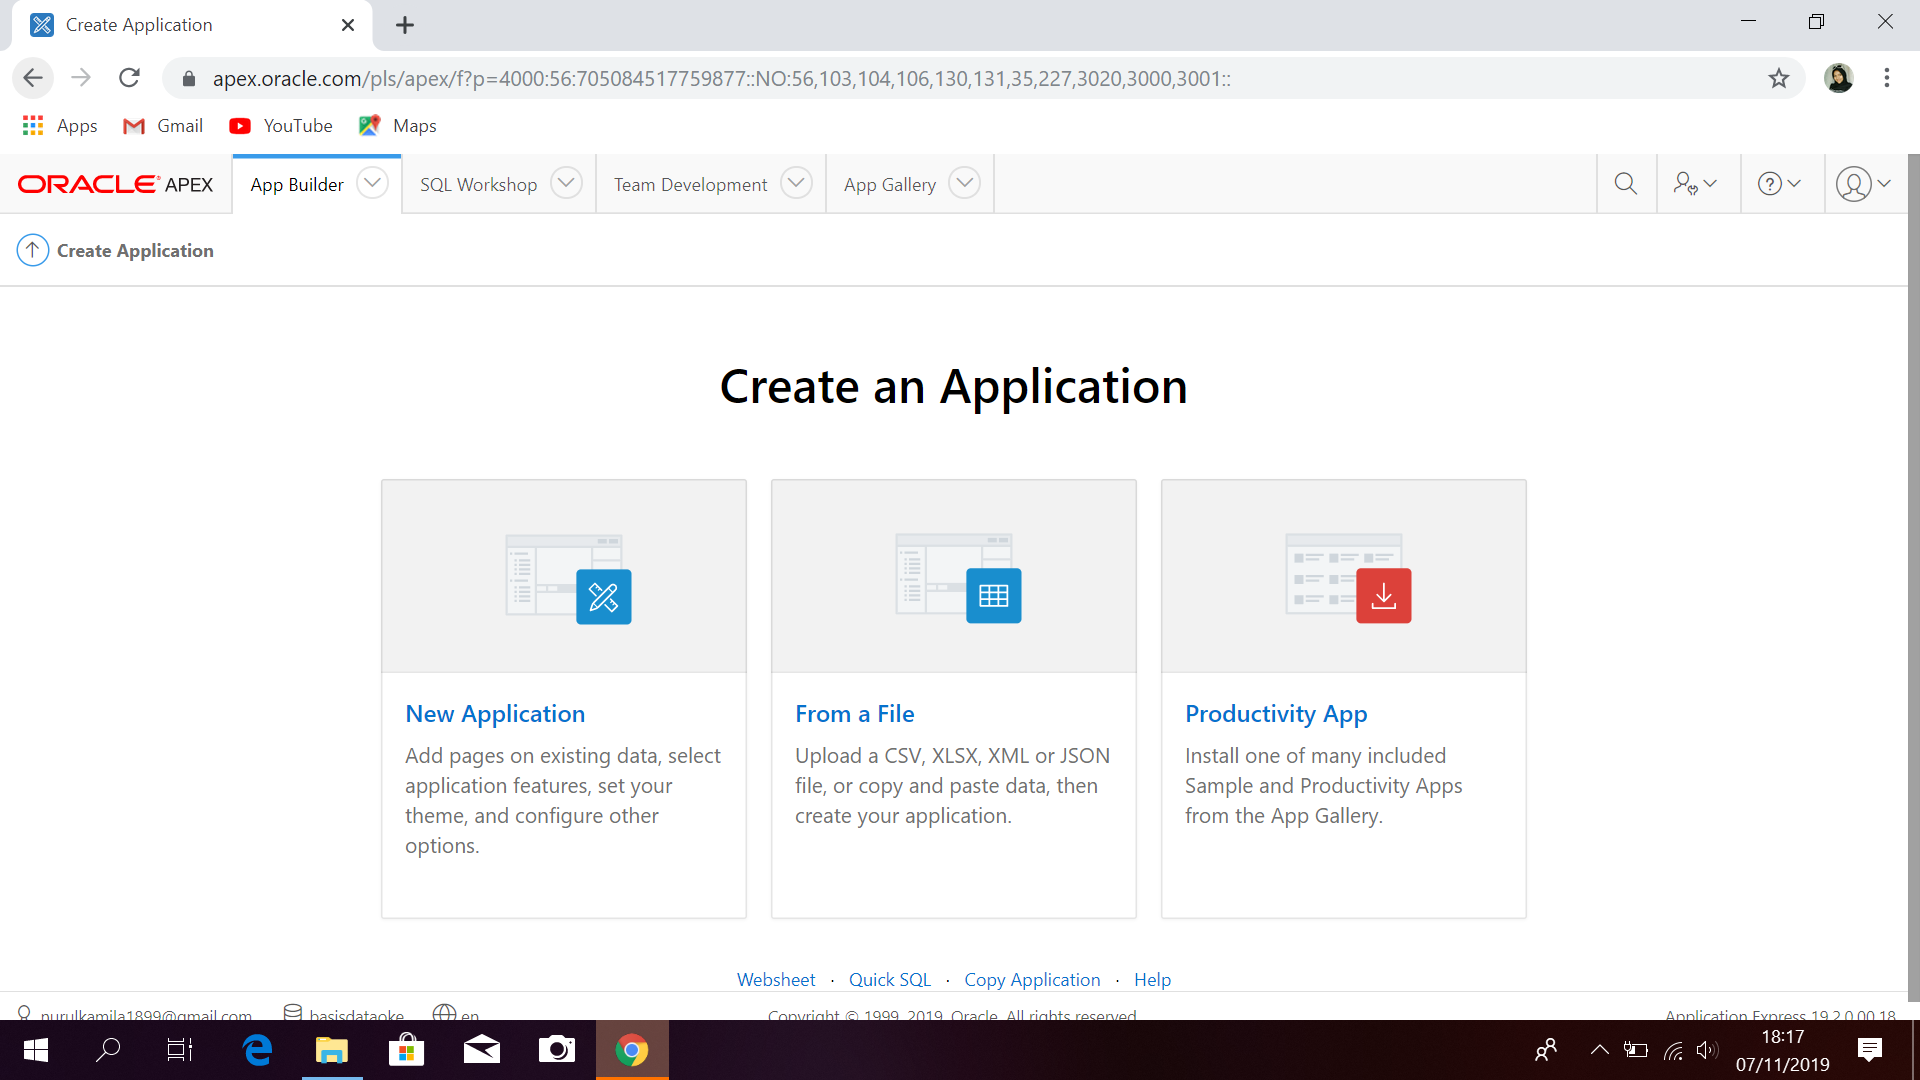
\includegraphics[width=.8\textwidth]{figure/2.PNG}
    \end{center}
    \item Lalu, klik Choose File dan pilih file exel yang berisikan data , seperti contoh di bawah ini
    \begin{center}
    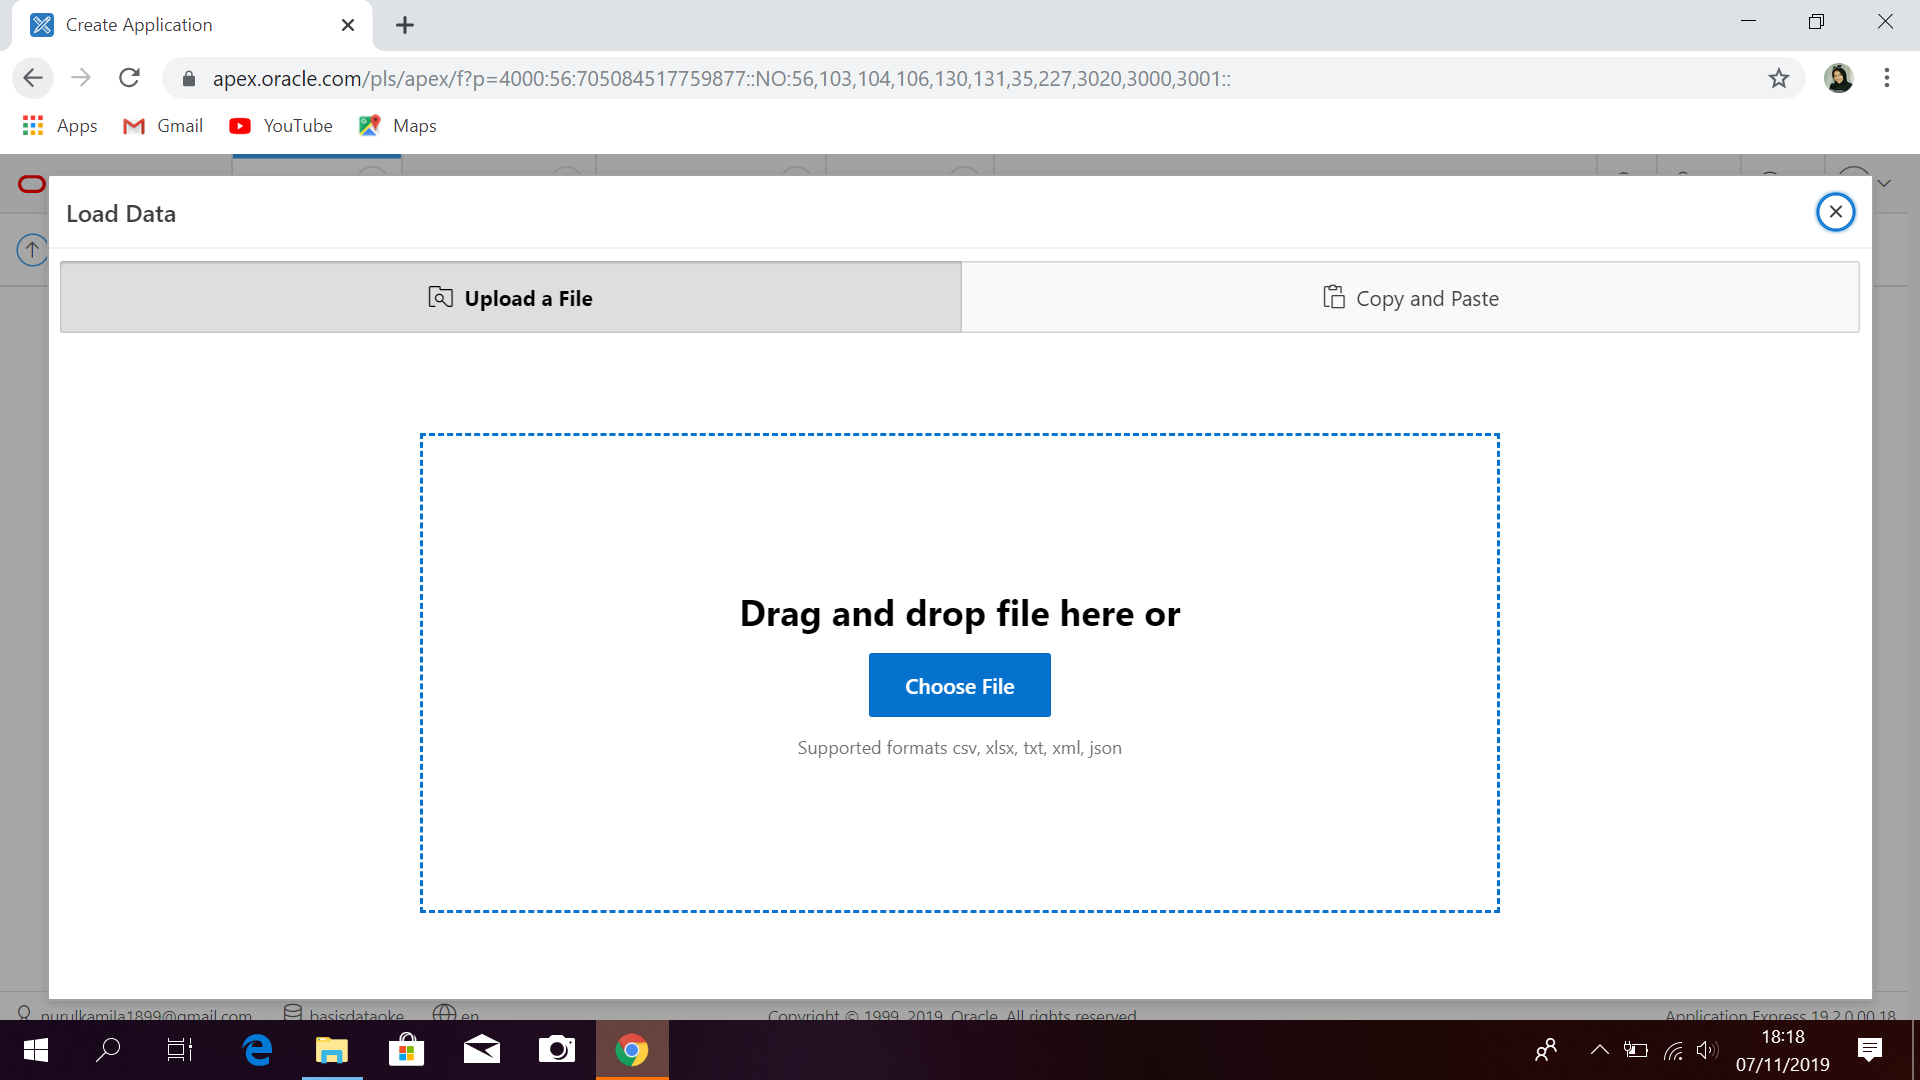
\includegraphics[width=.8\textwidth]{figure/3.PNG}
    \end{center}
    \item Pada laman selanjutnya, silahkan masukkan nama Table sesuai yang kamu inginkan, perlu diketahui pada kolom error table name akan terisi otomatis. setelah itu klik Configure, lalu save change.
    \begin{center}
    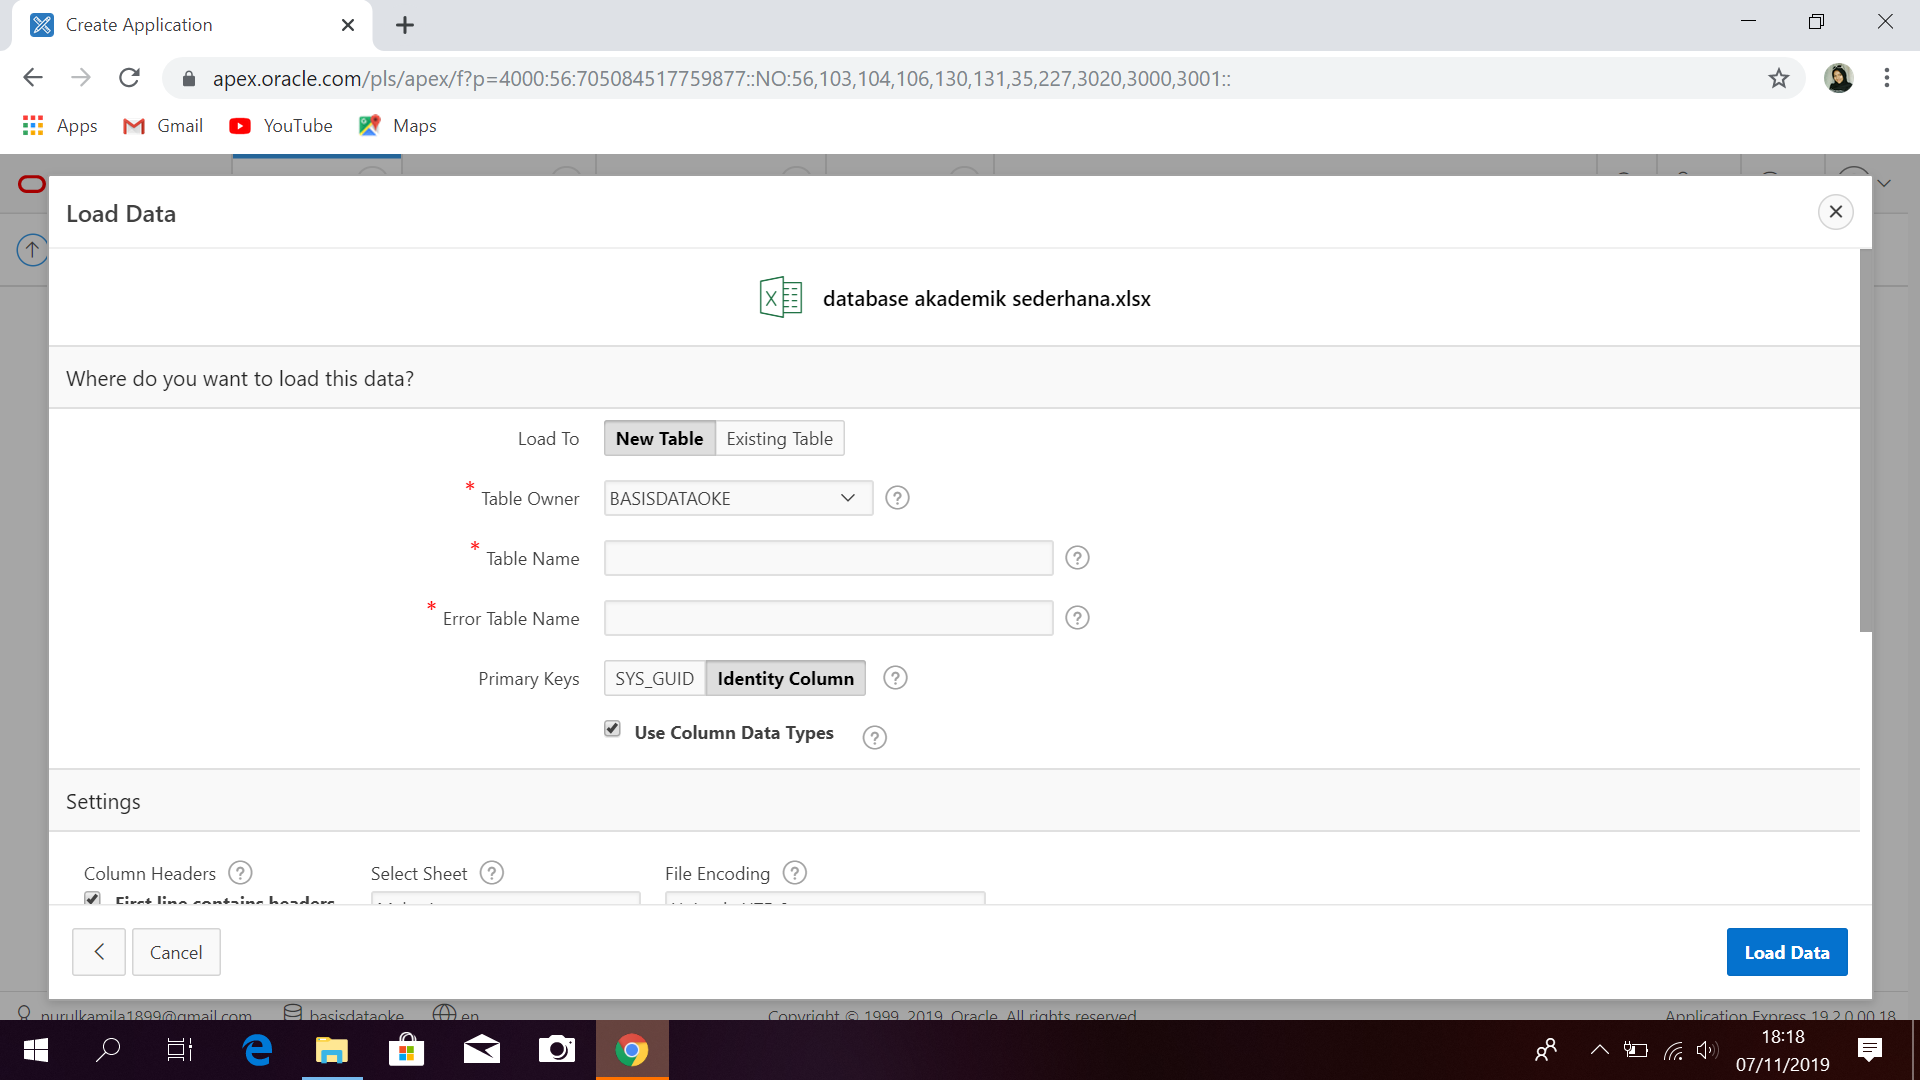
\includegraphics[width=.8\textwidth]{figure/4.PNG}
    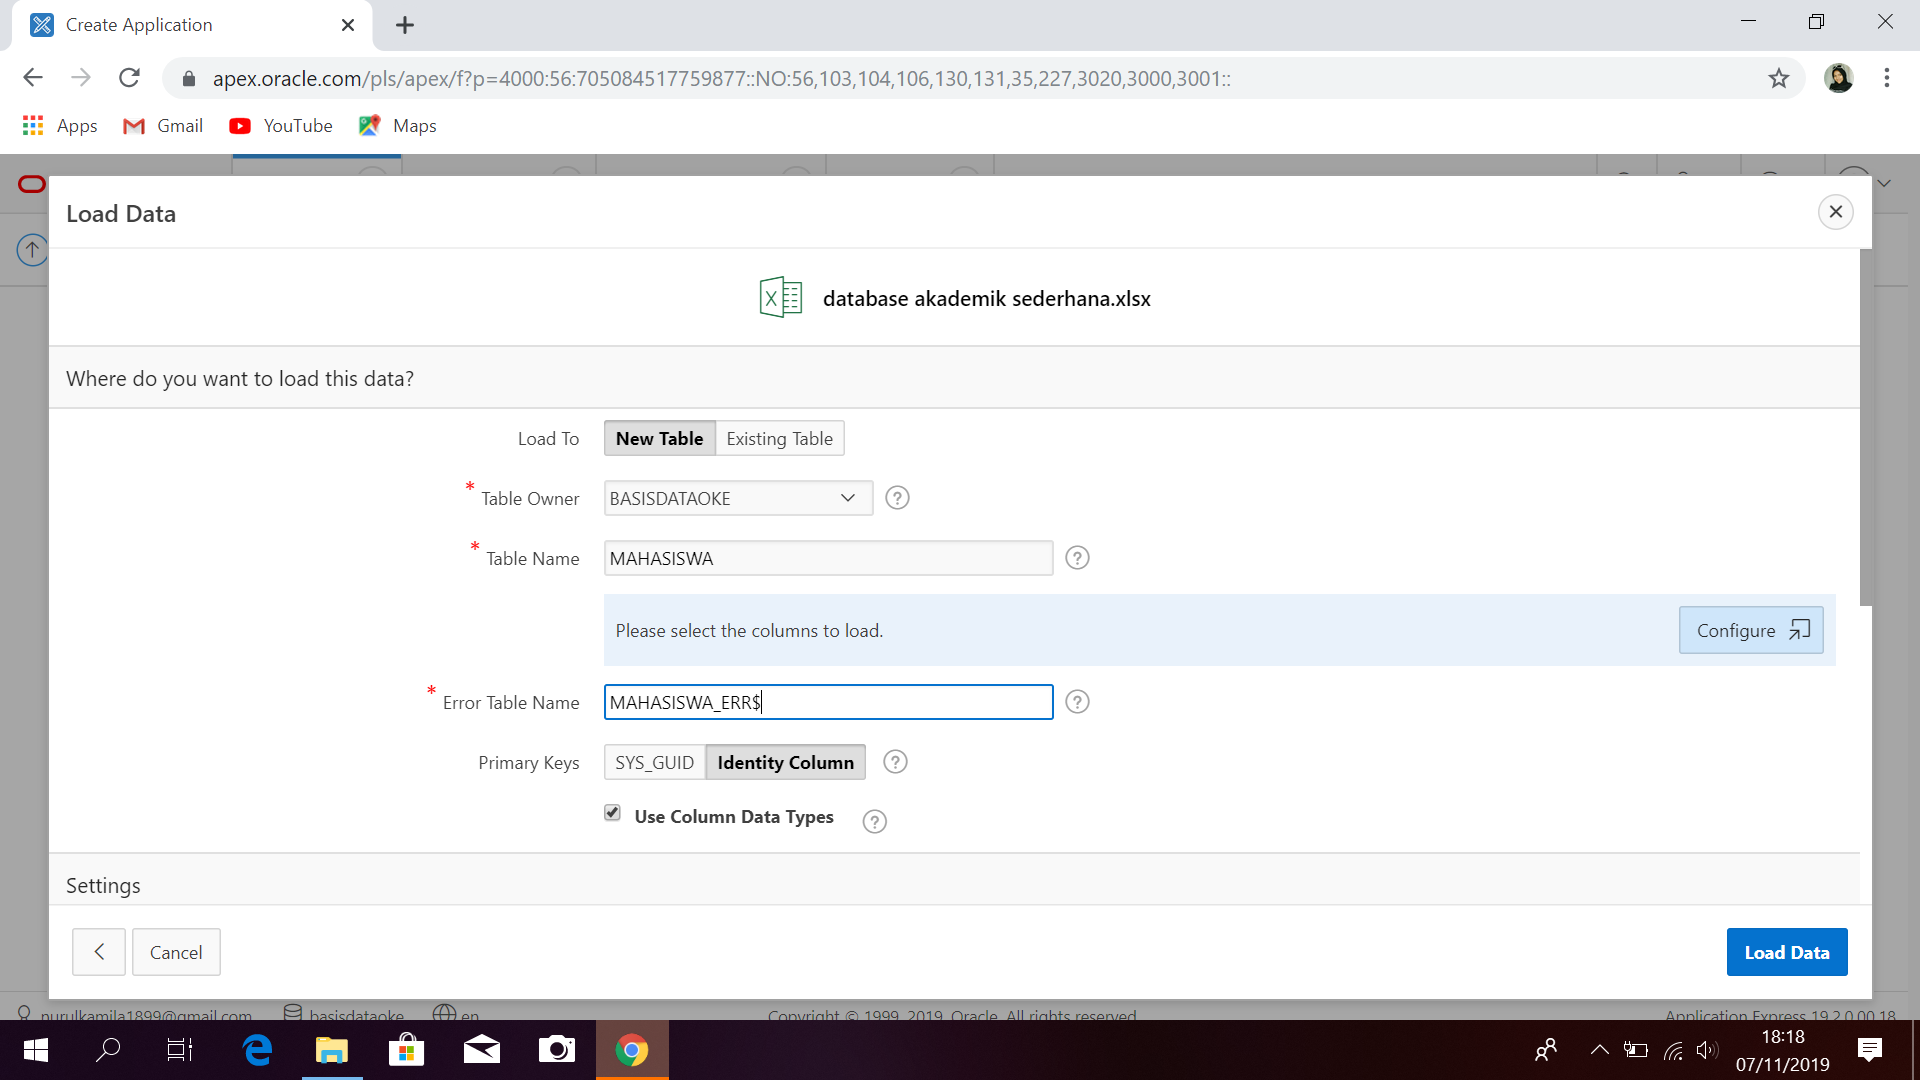
\includegraphics[width=.8\textwidth]{figure/5.PNG}
    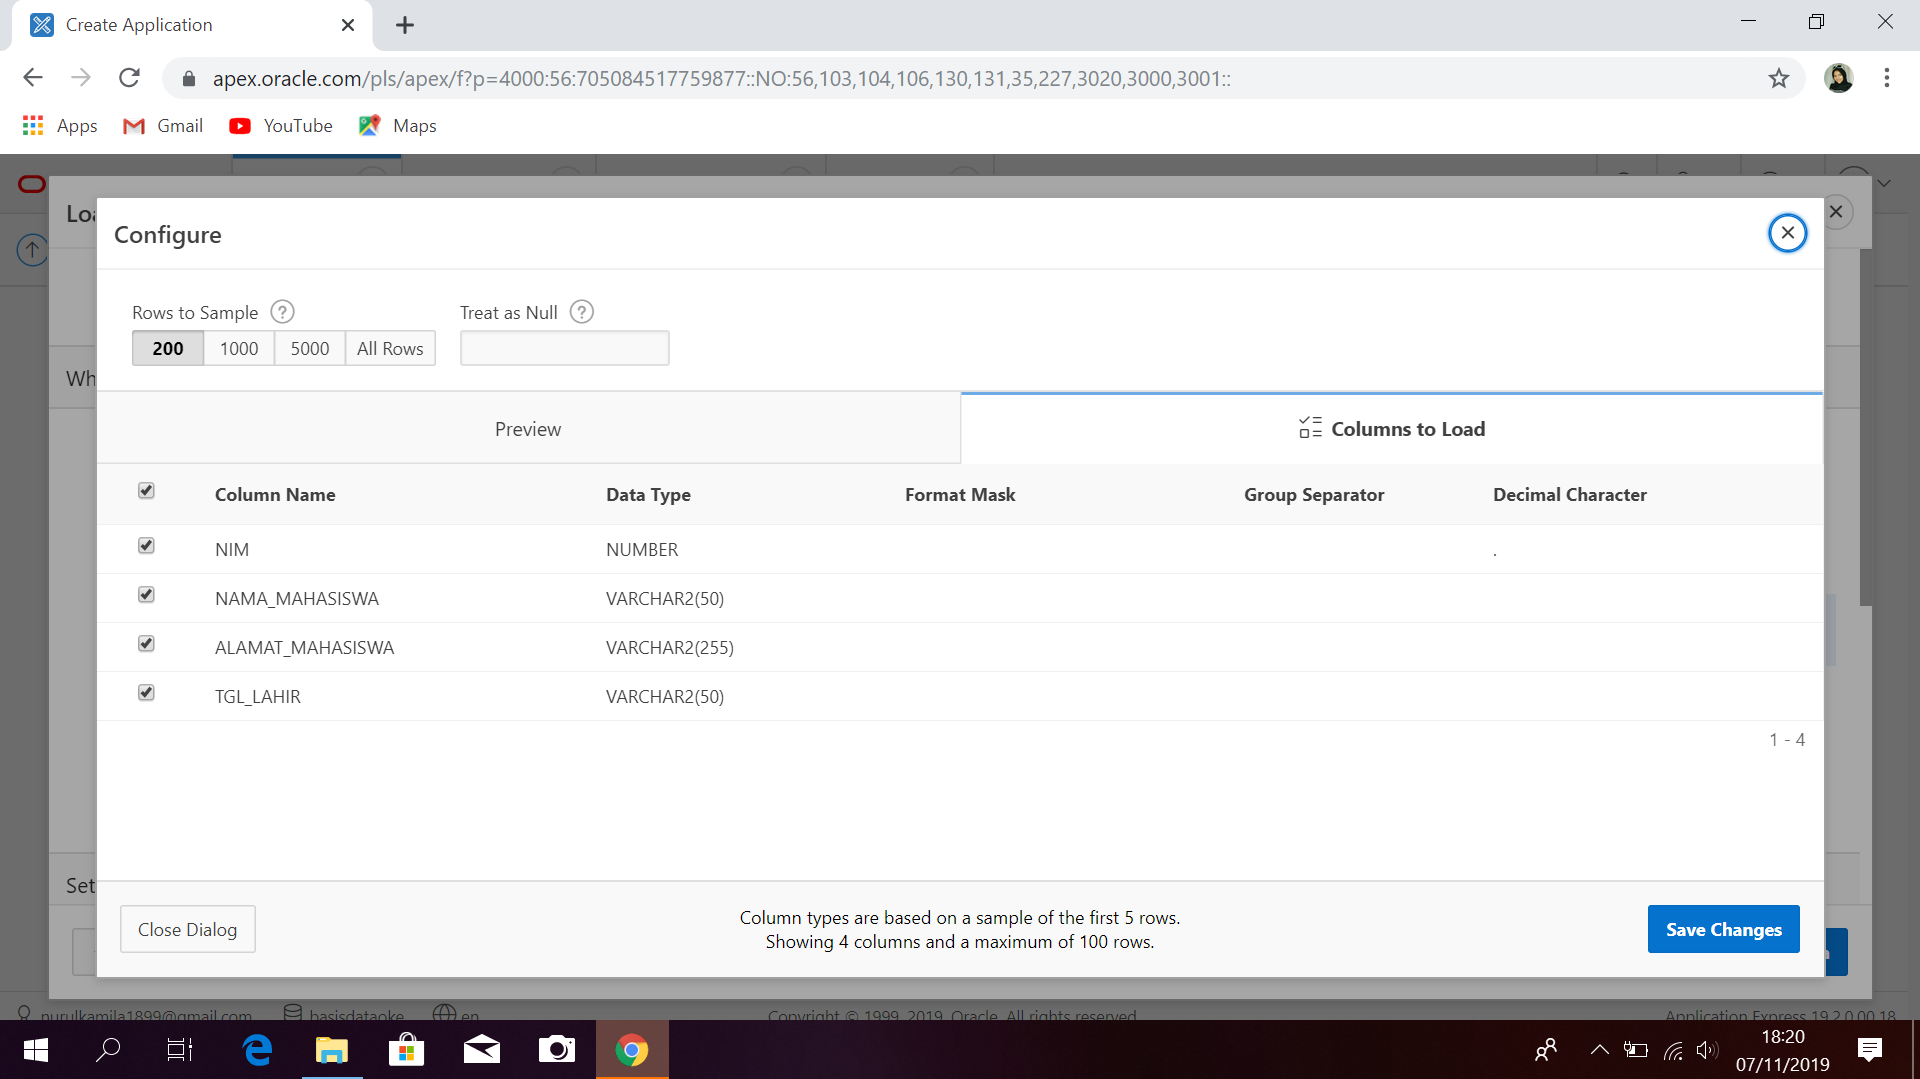
\includegraphics[width=.8\textwidth]{figure/6.PNG}
    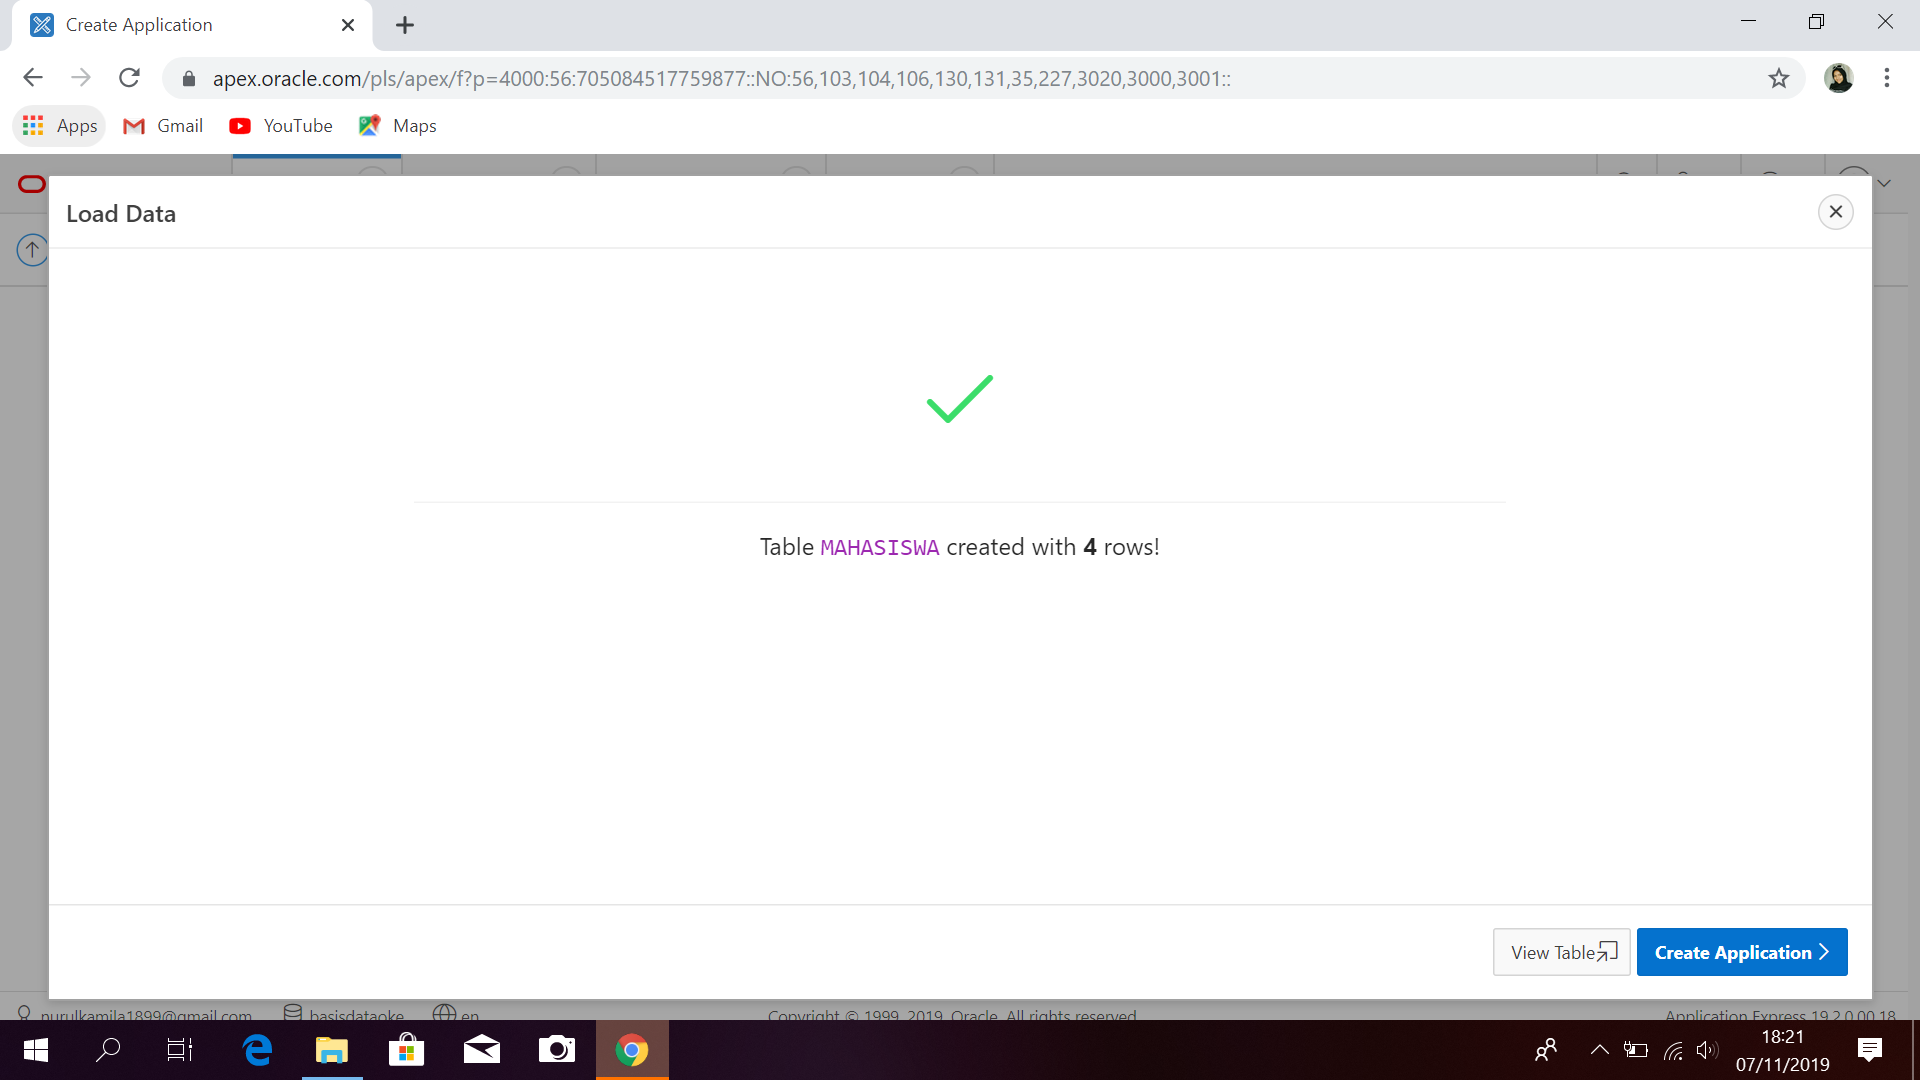
\includegraphics[width=.8\textwidth]{figure/7.PNG}
    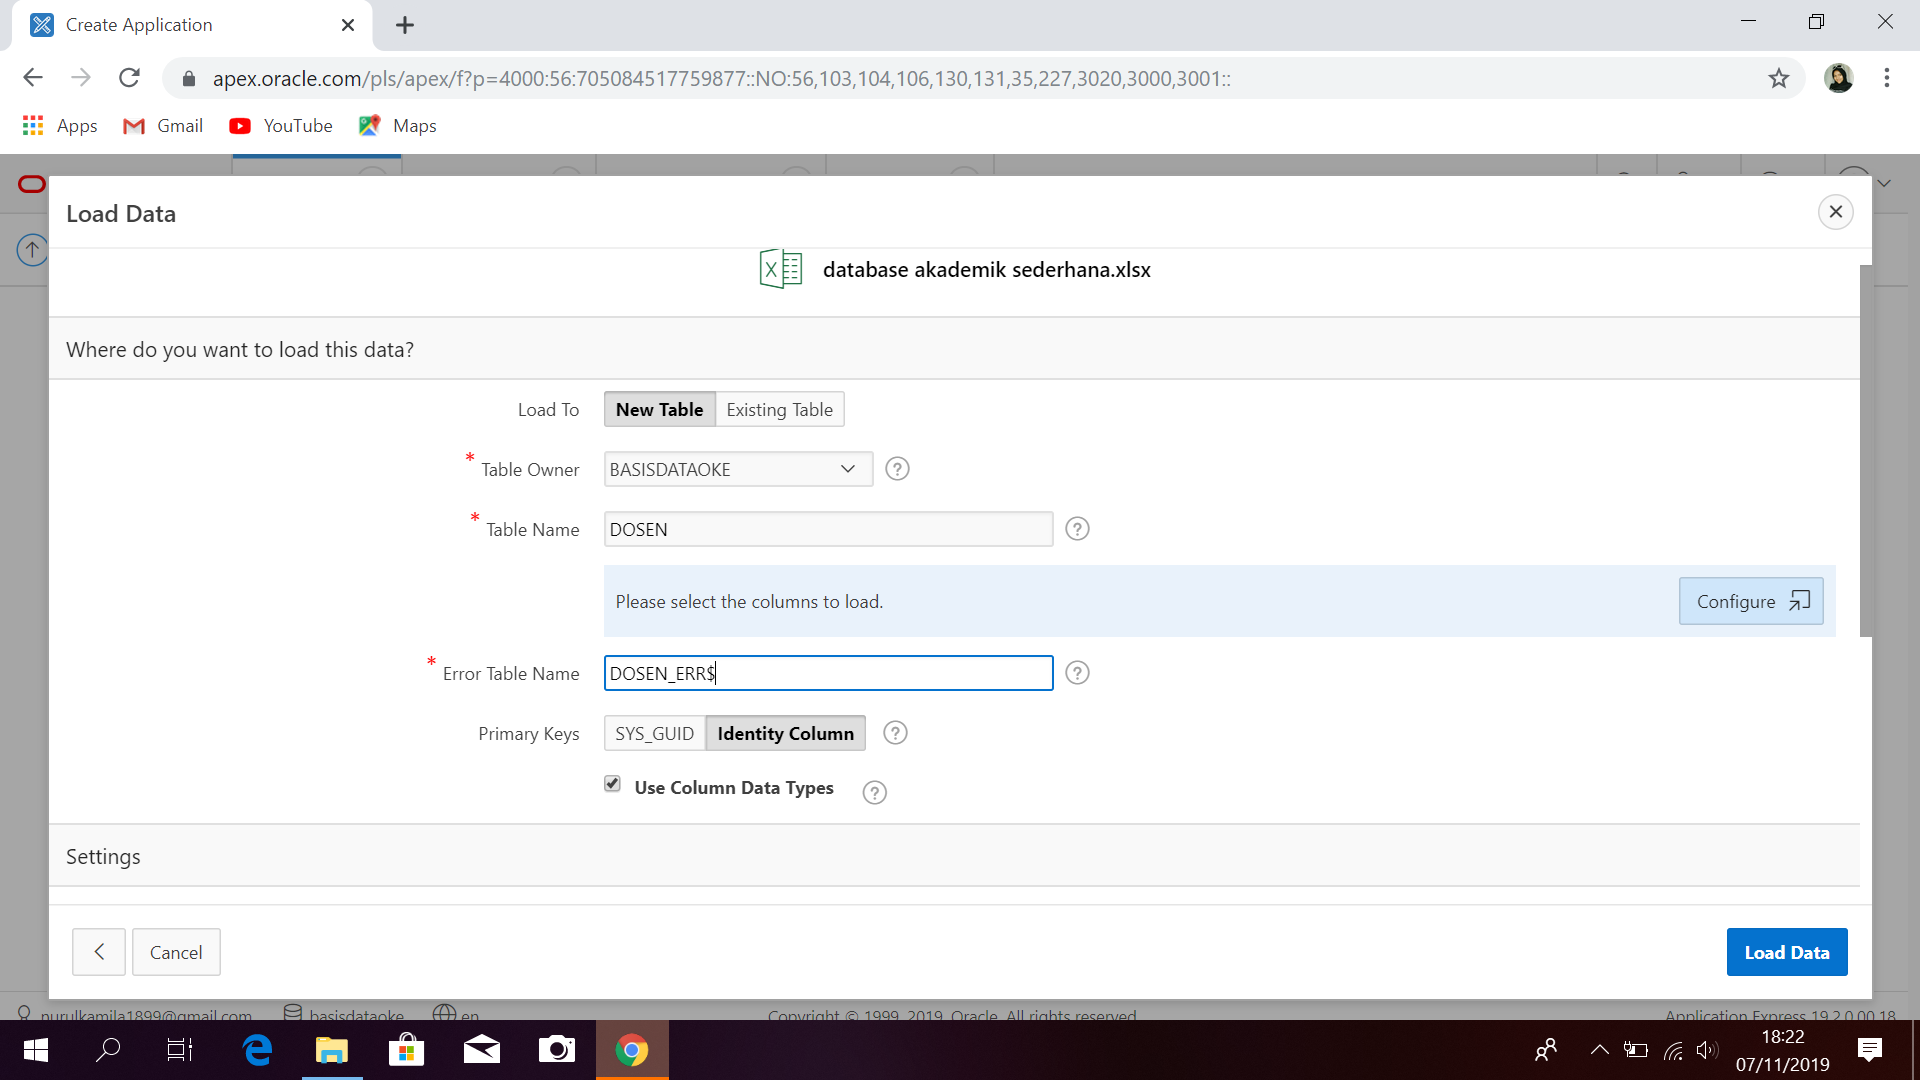
\includegraphics[width=.8\textwidth]{figure/8.PNG}
    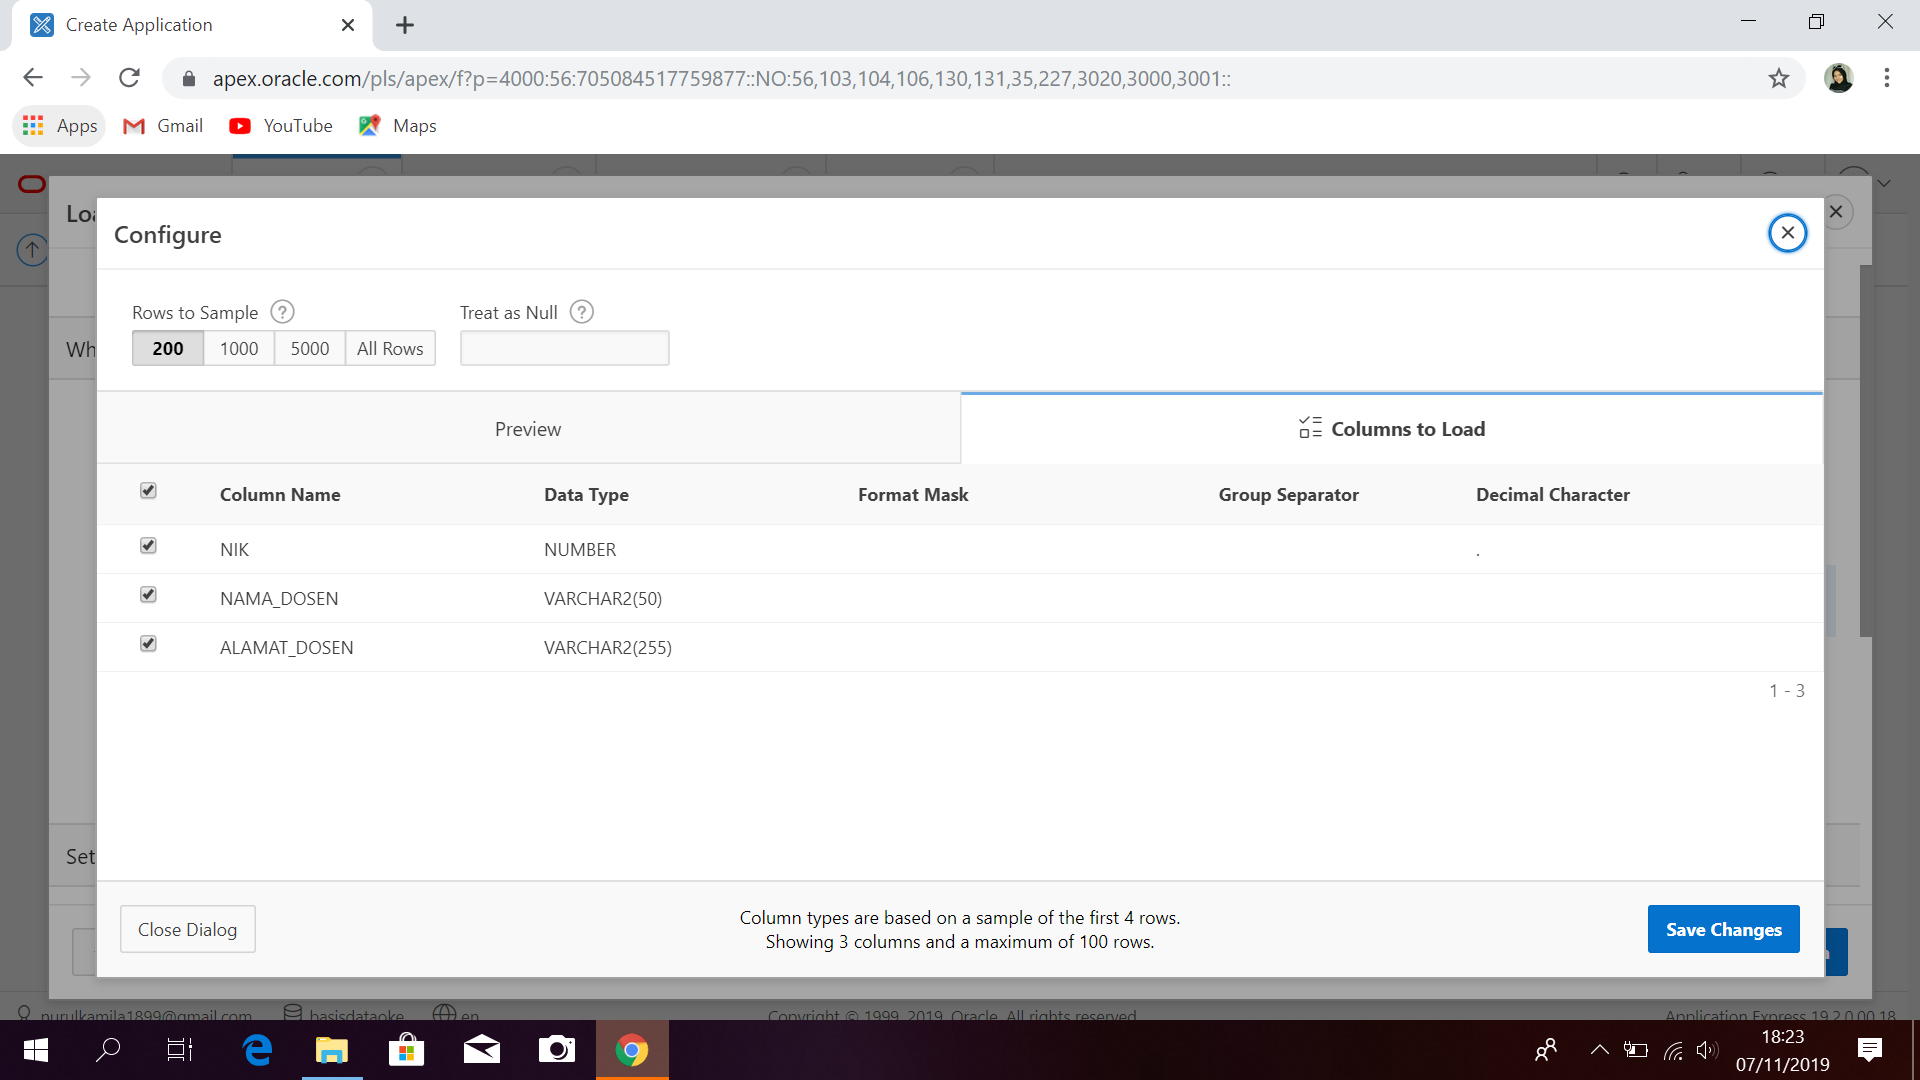
\includegraphics[width=.8\textwidth]{figure/9.PNG}
    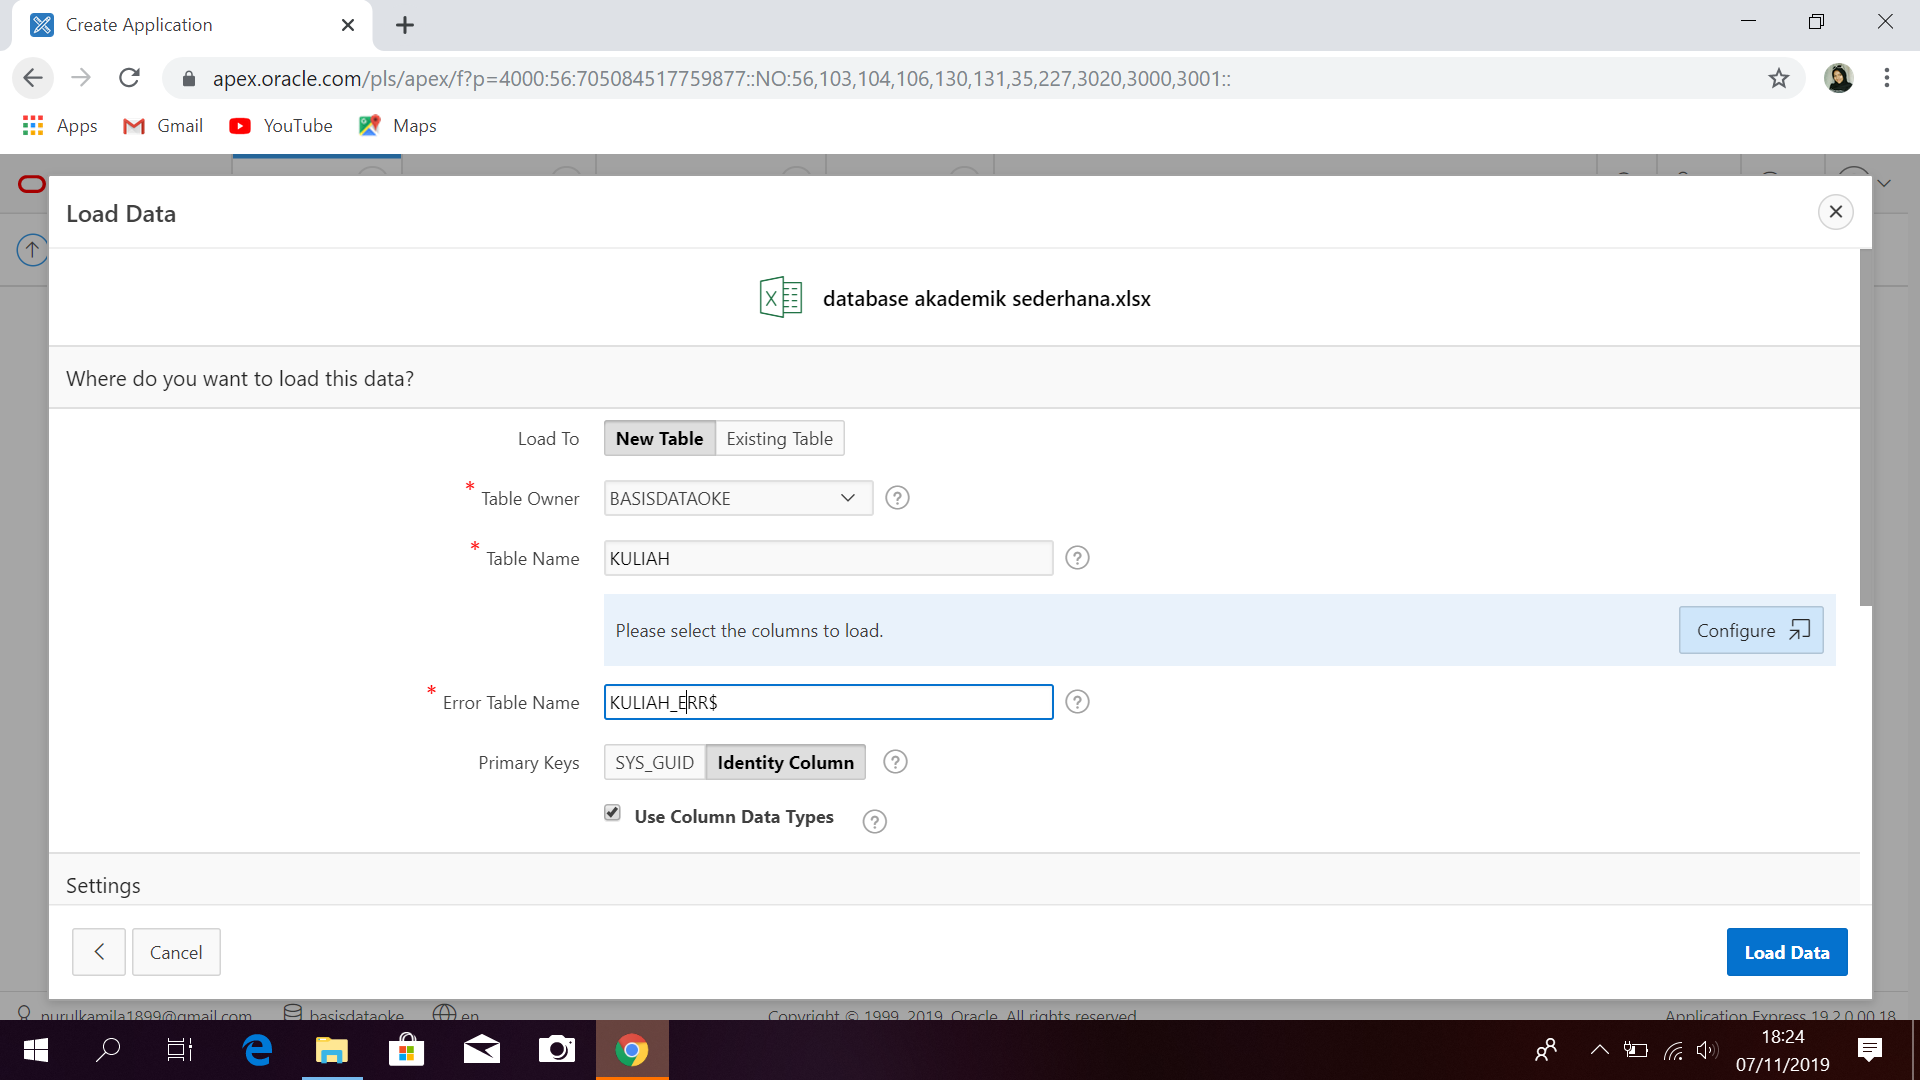
\includegraphics[width=.8\textwidth]{figure/10.PNG}
    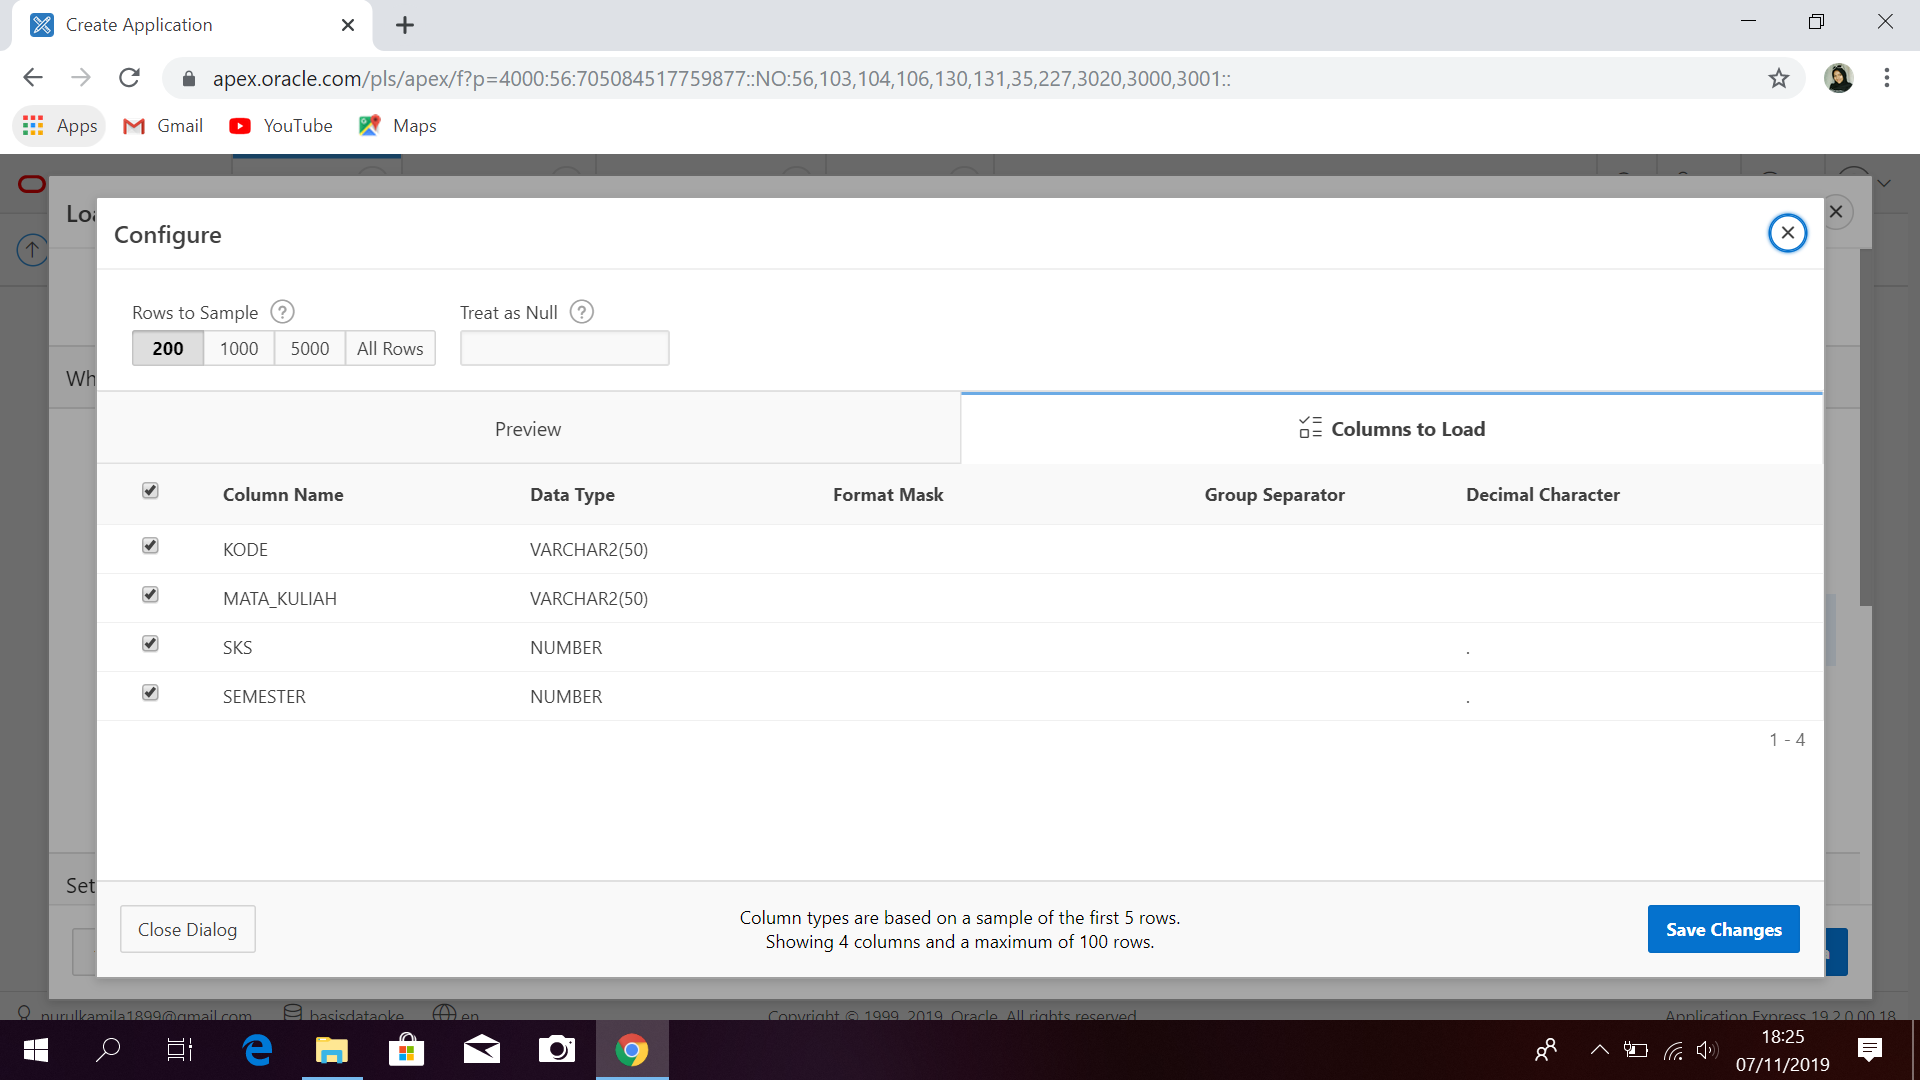
\includegraphics[width=.8\textwidth]{figure/11.PNG}
    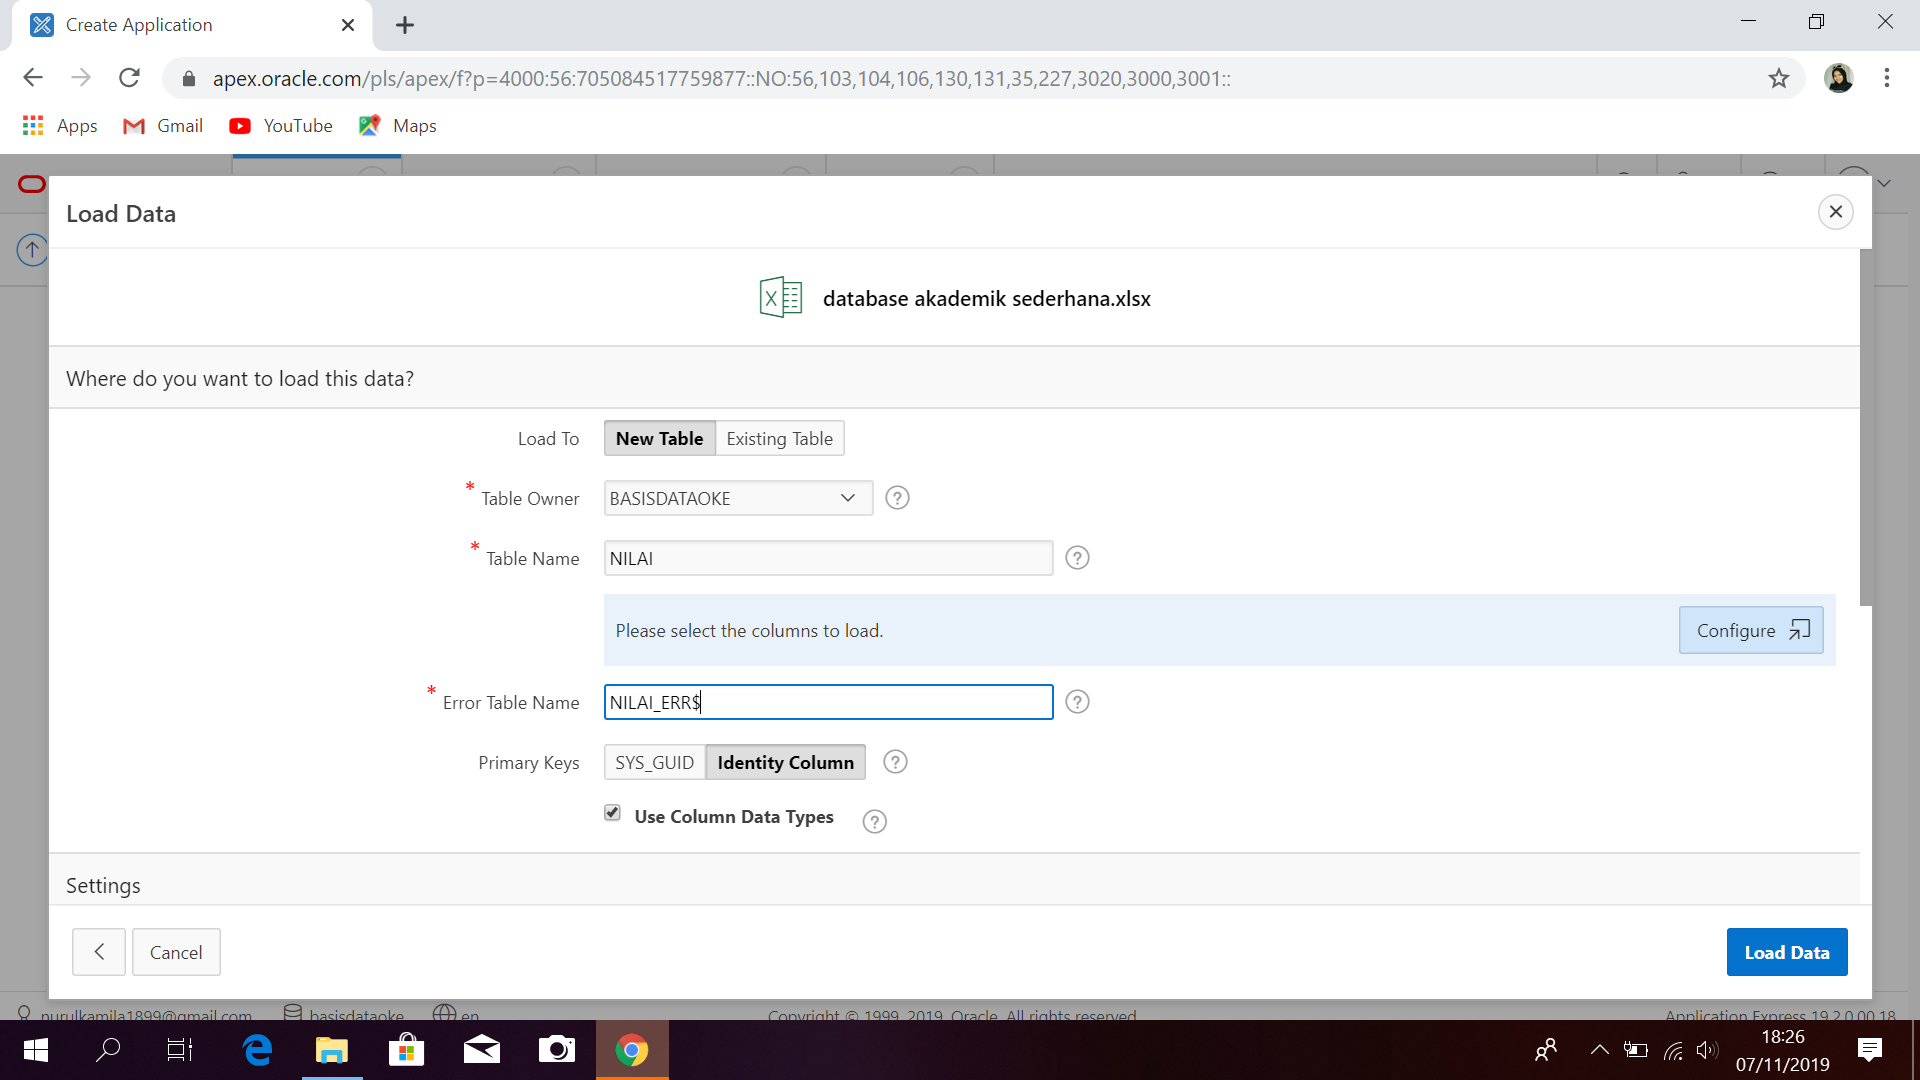
\includegraphics[width=.8\textwidth]{figure/12.PNG}
    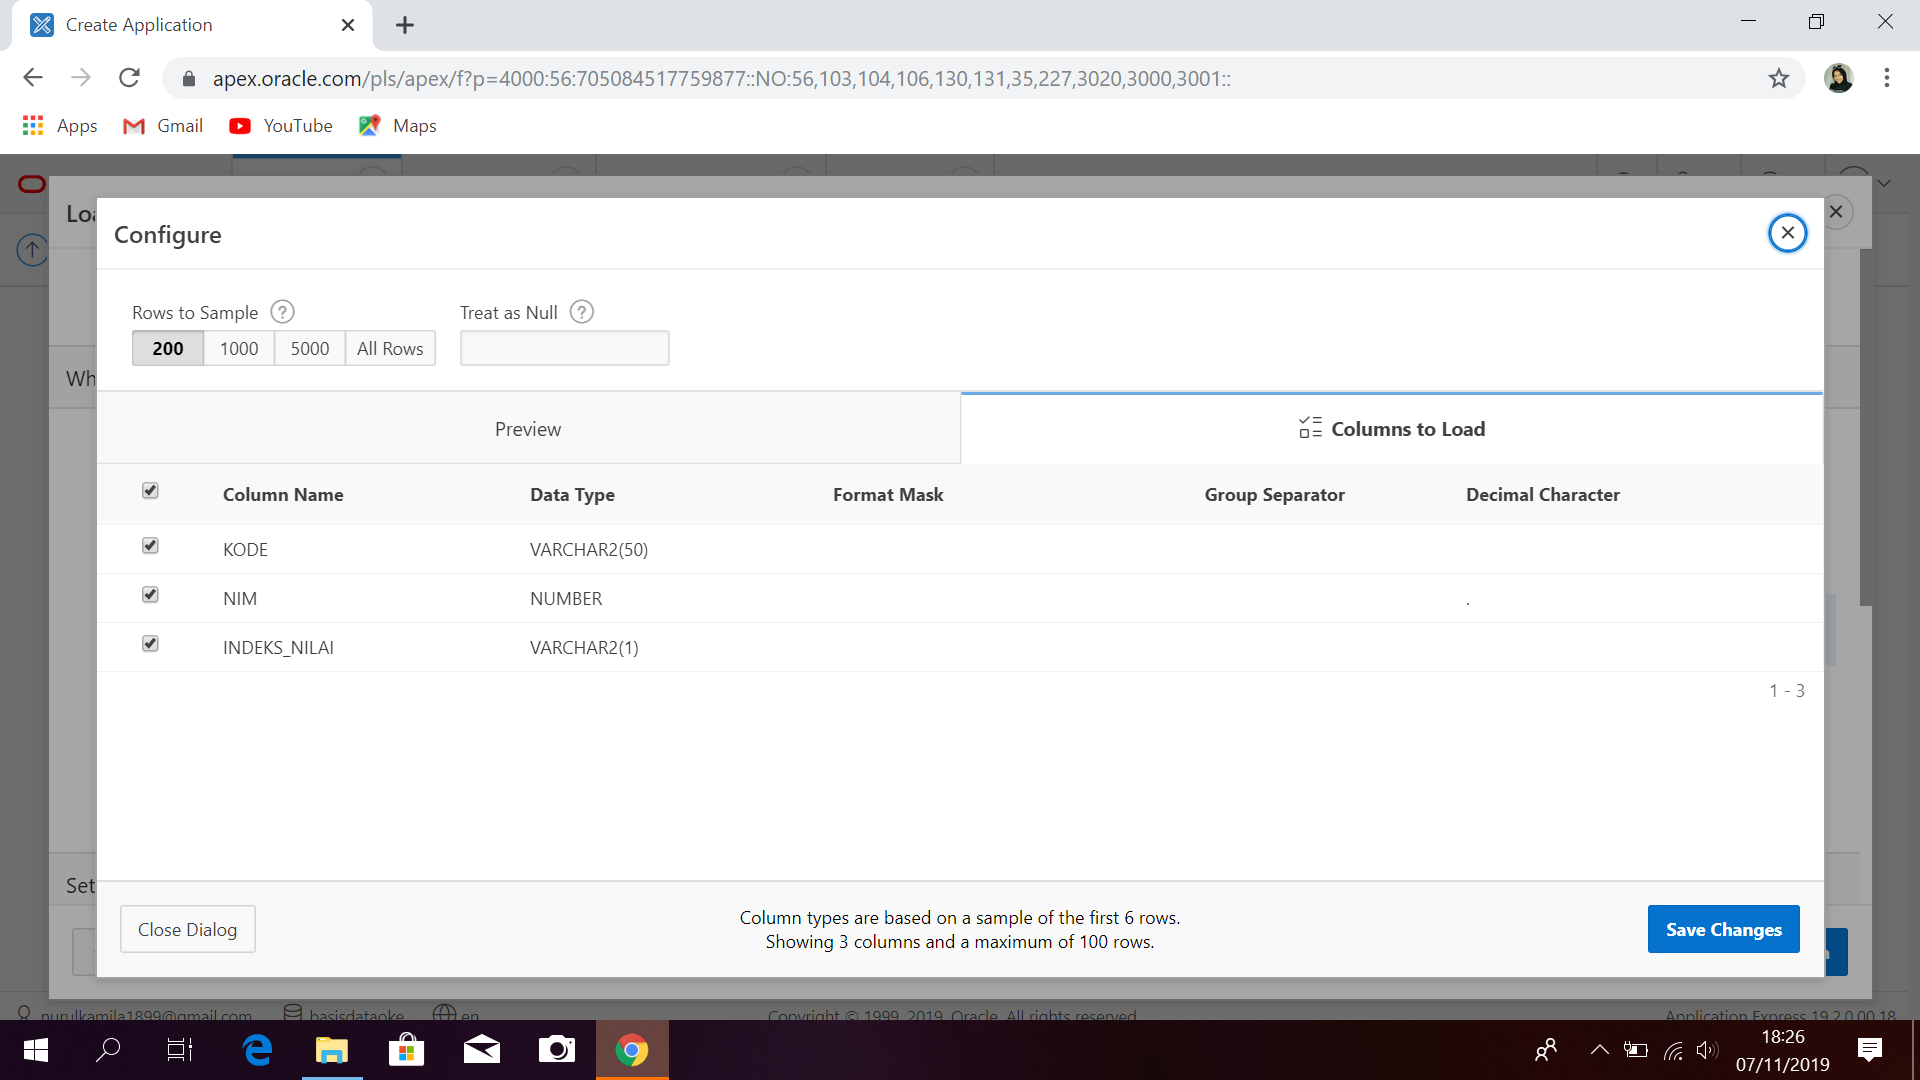
\includegraphics[width=.8\textwidth]{figure/13.PNG}
    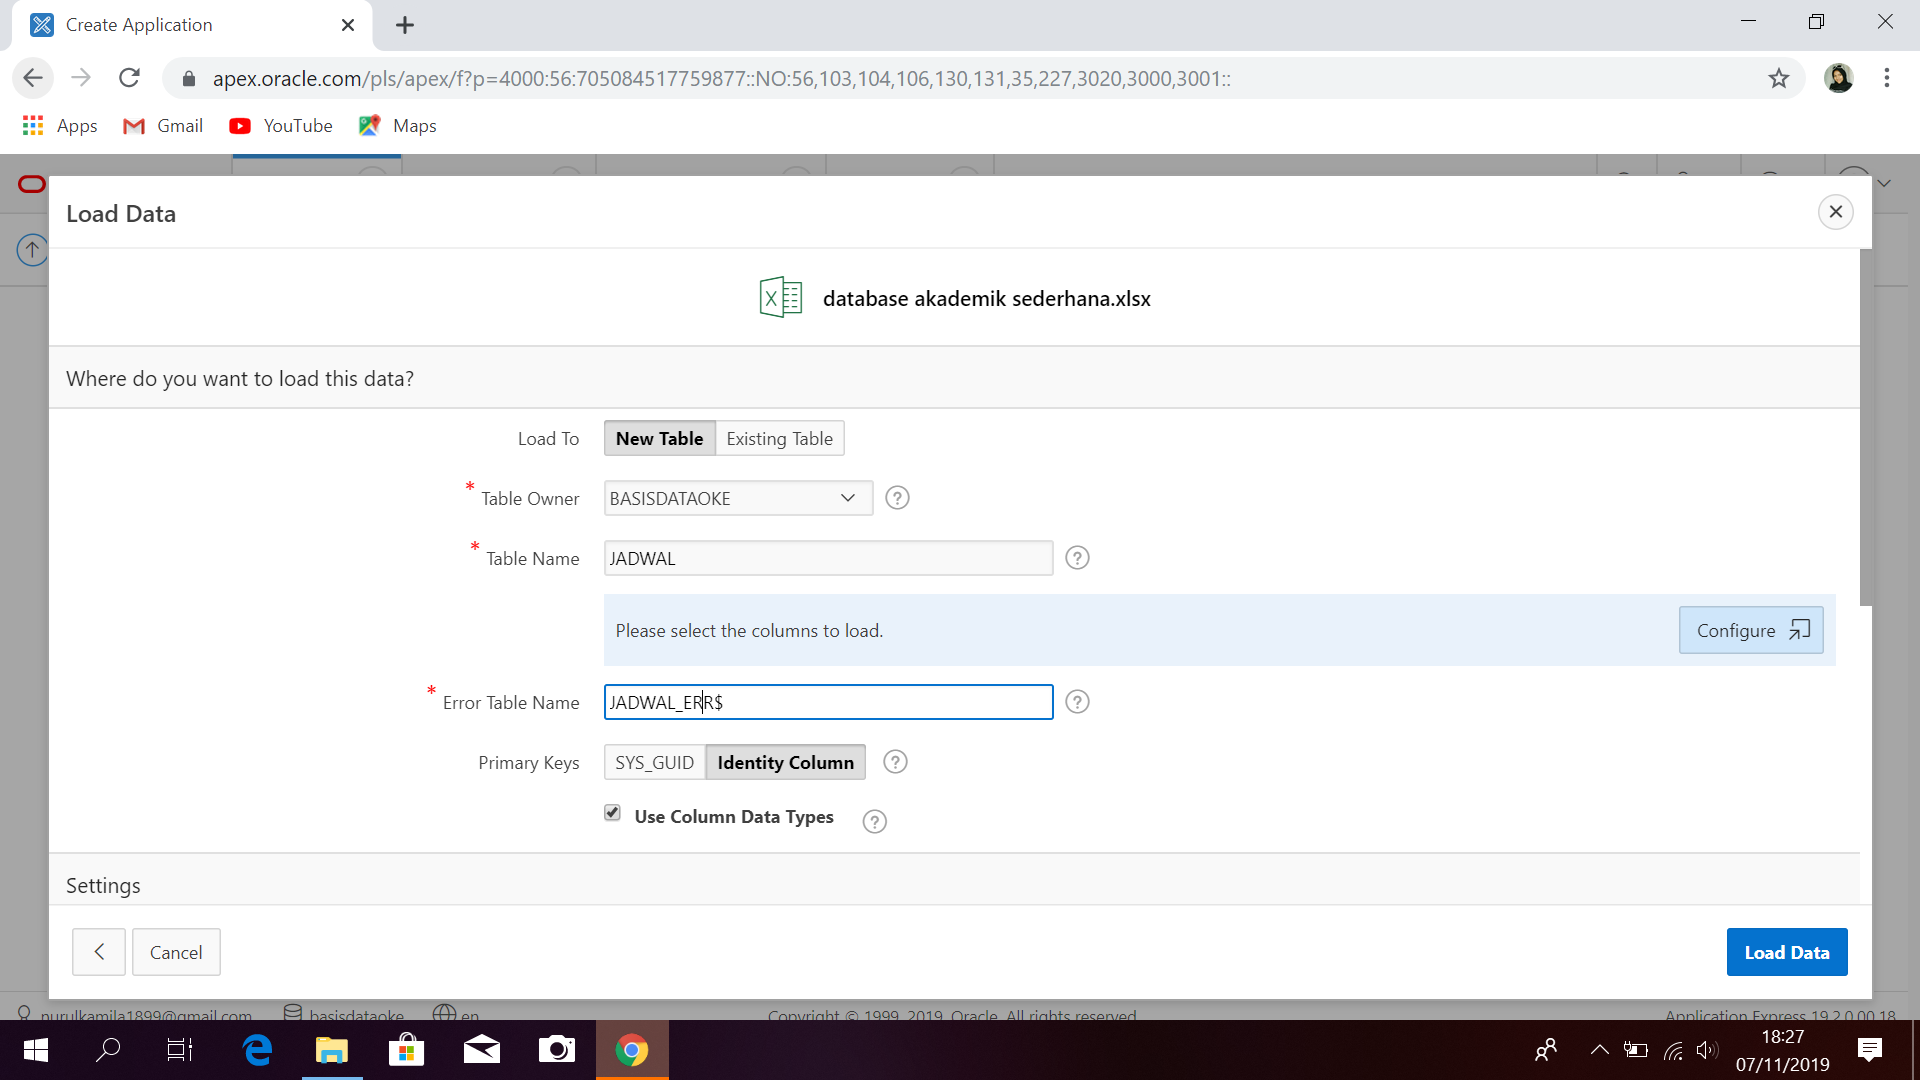
\includegraphics[width=.8\textwidth]{figure/14.PNG}
    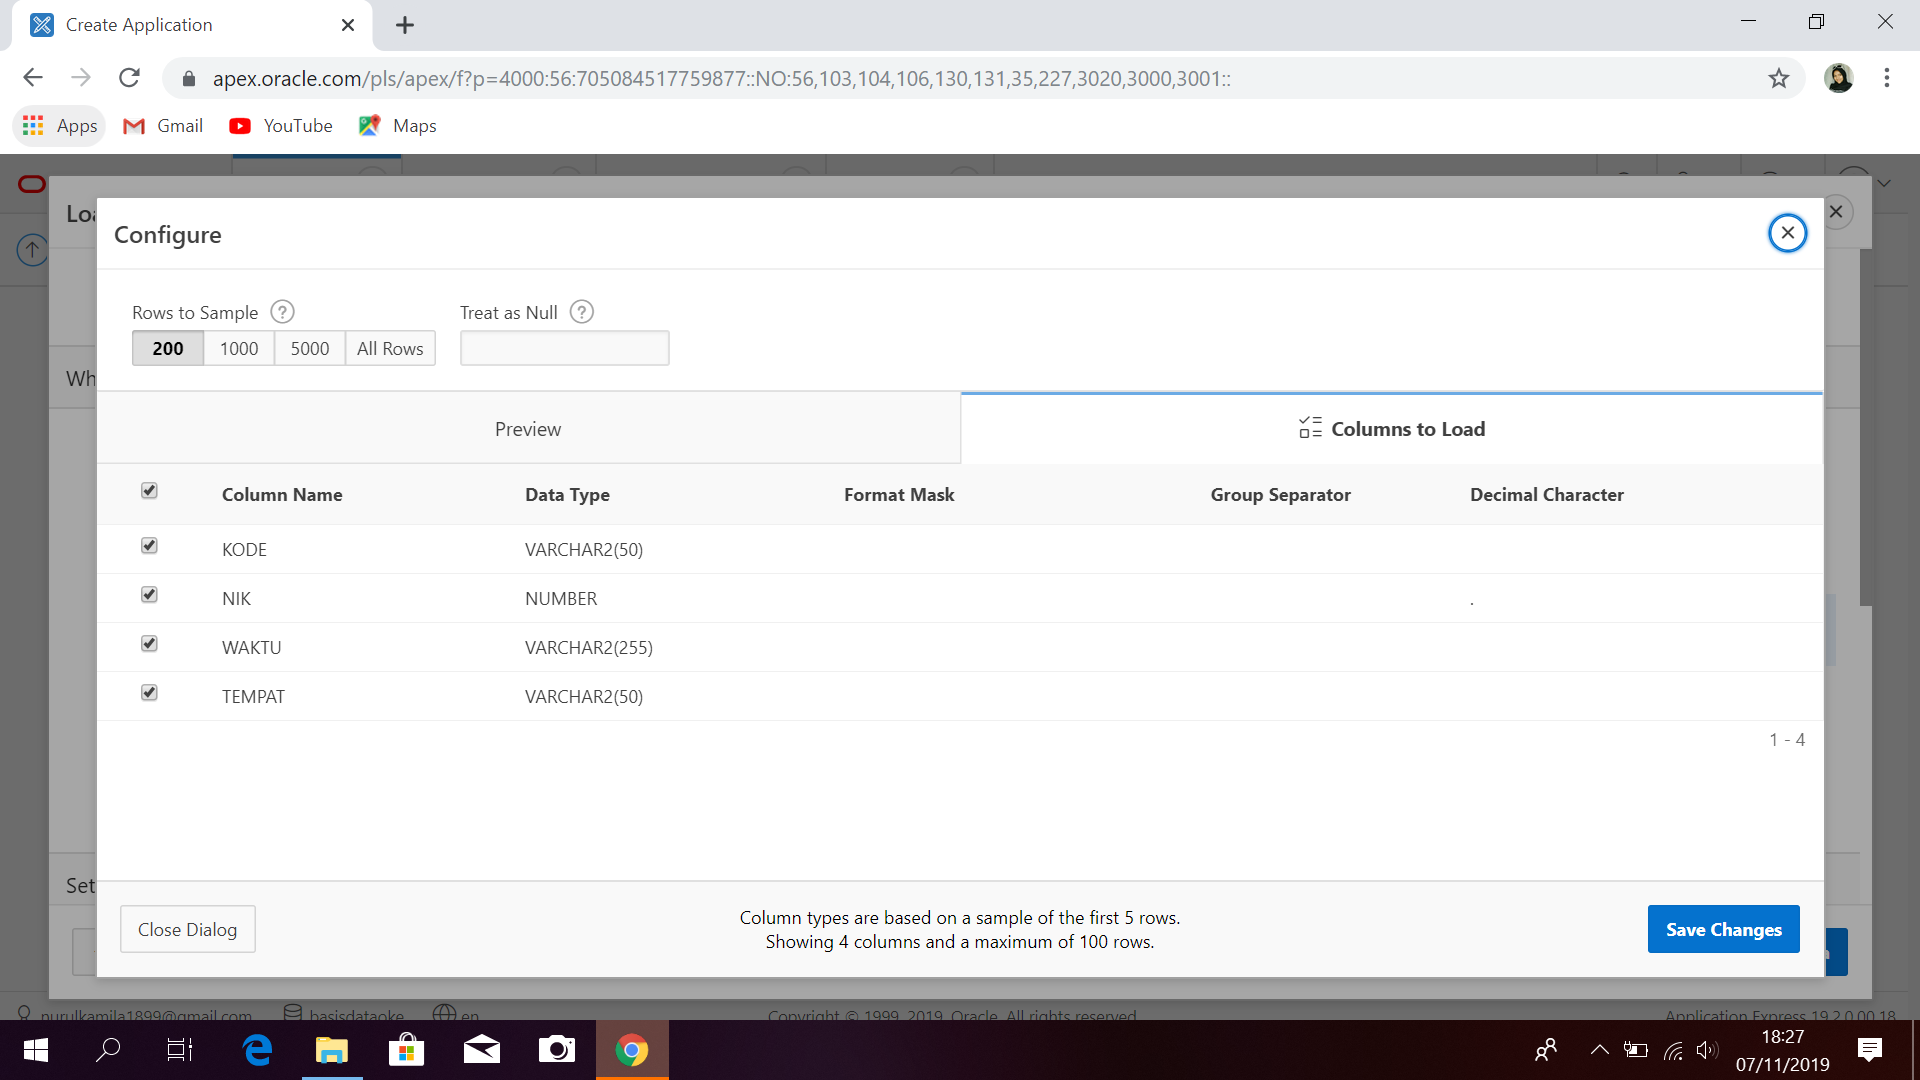
\includegraphics[width=.8\textwidth]{figure/15.PNG}
    \end{center}
    \item Kita dapat melihat table kita pada SQL WorkShop
     \begin{center}
    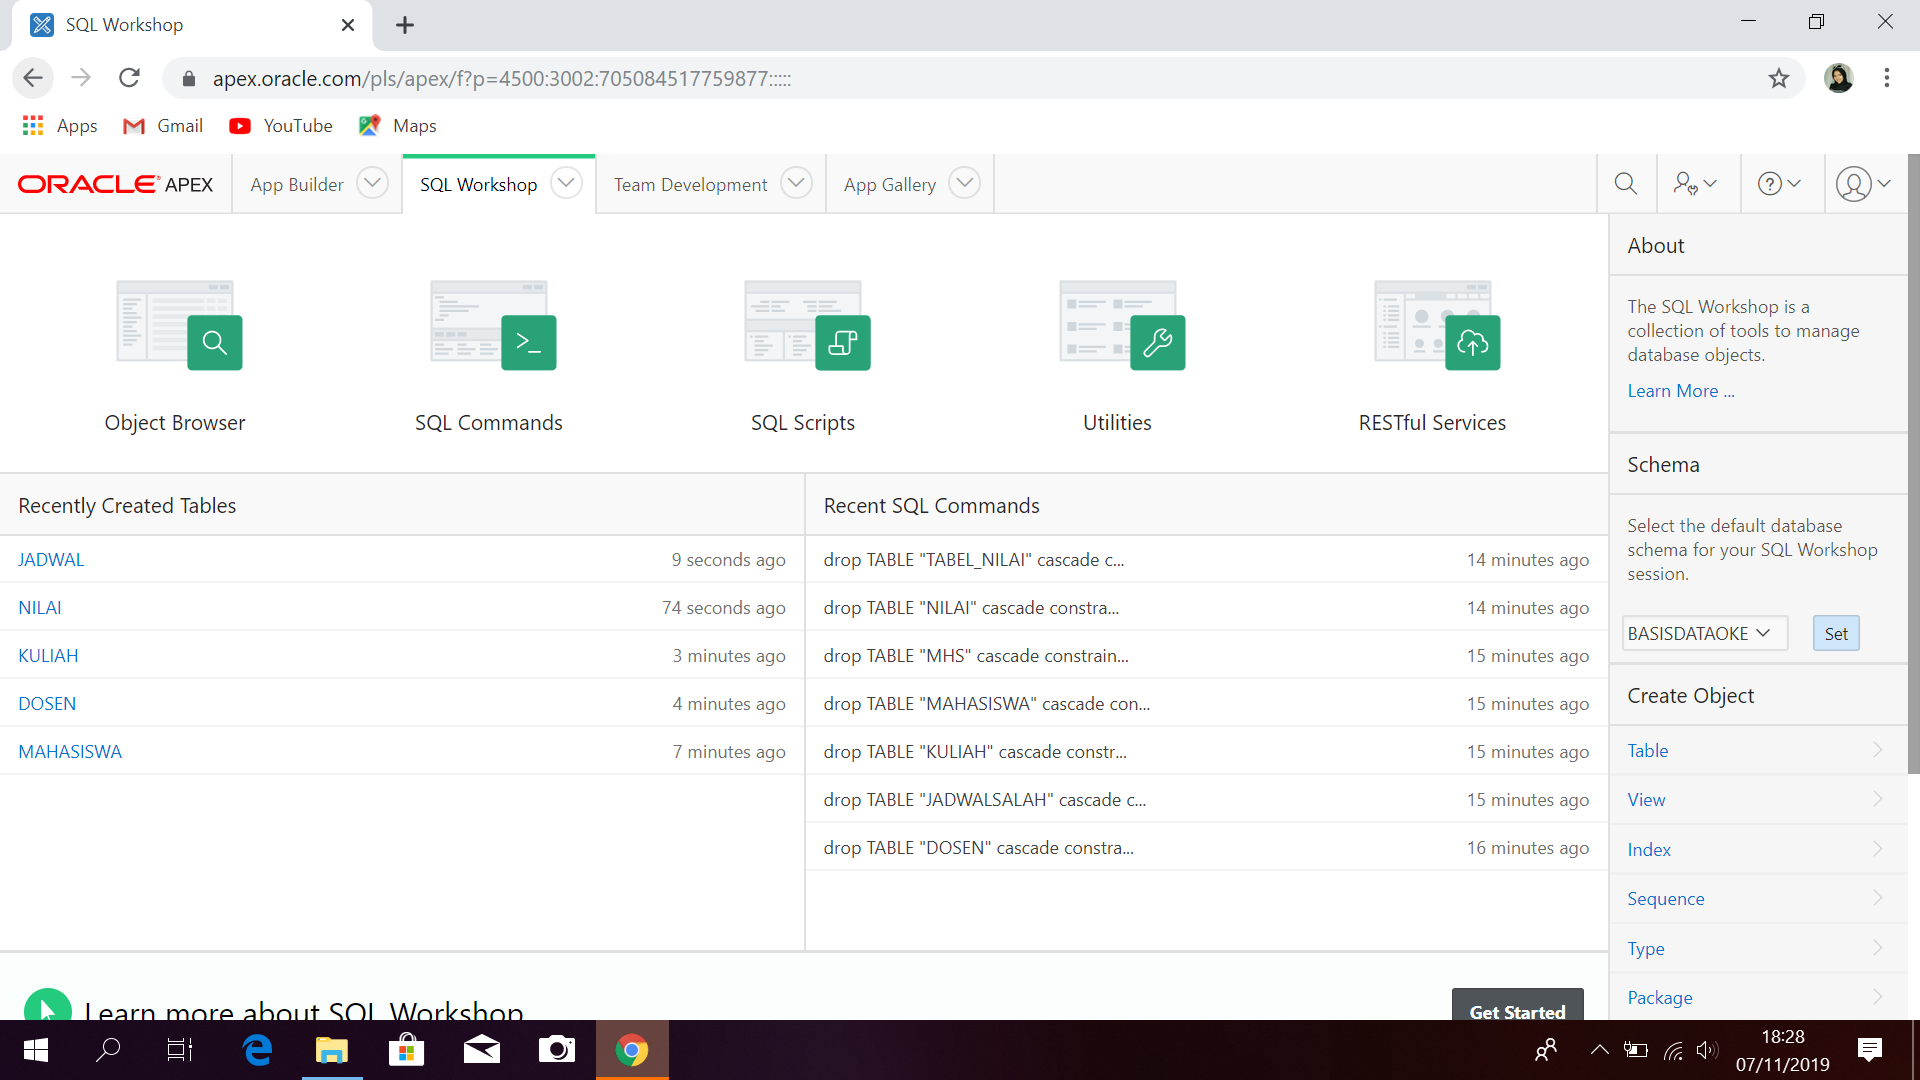
\includegraphics[width=.8\textwidth]{figure/16.PNG}
    \end{center}
    \item Kemudian Kita Hilangkan kolom ID(number) pada setiap tabel tersebut
     \begin{center}
    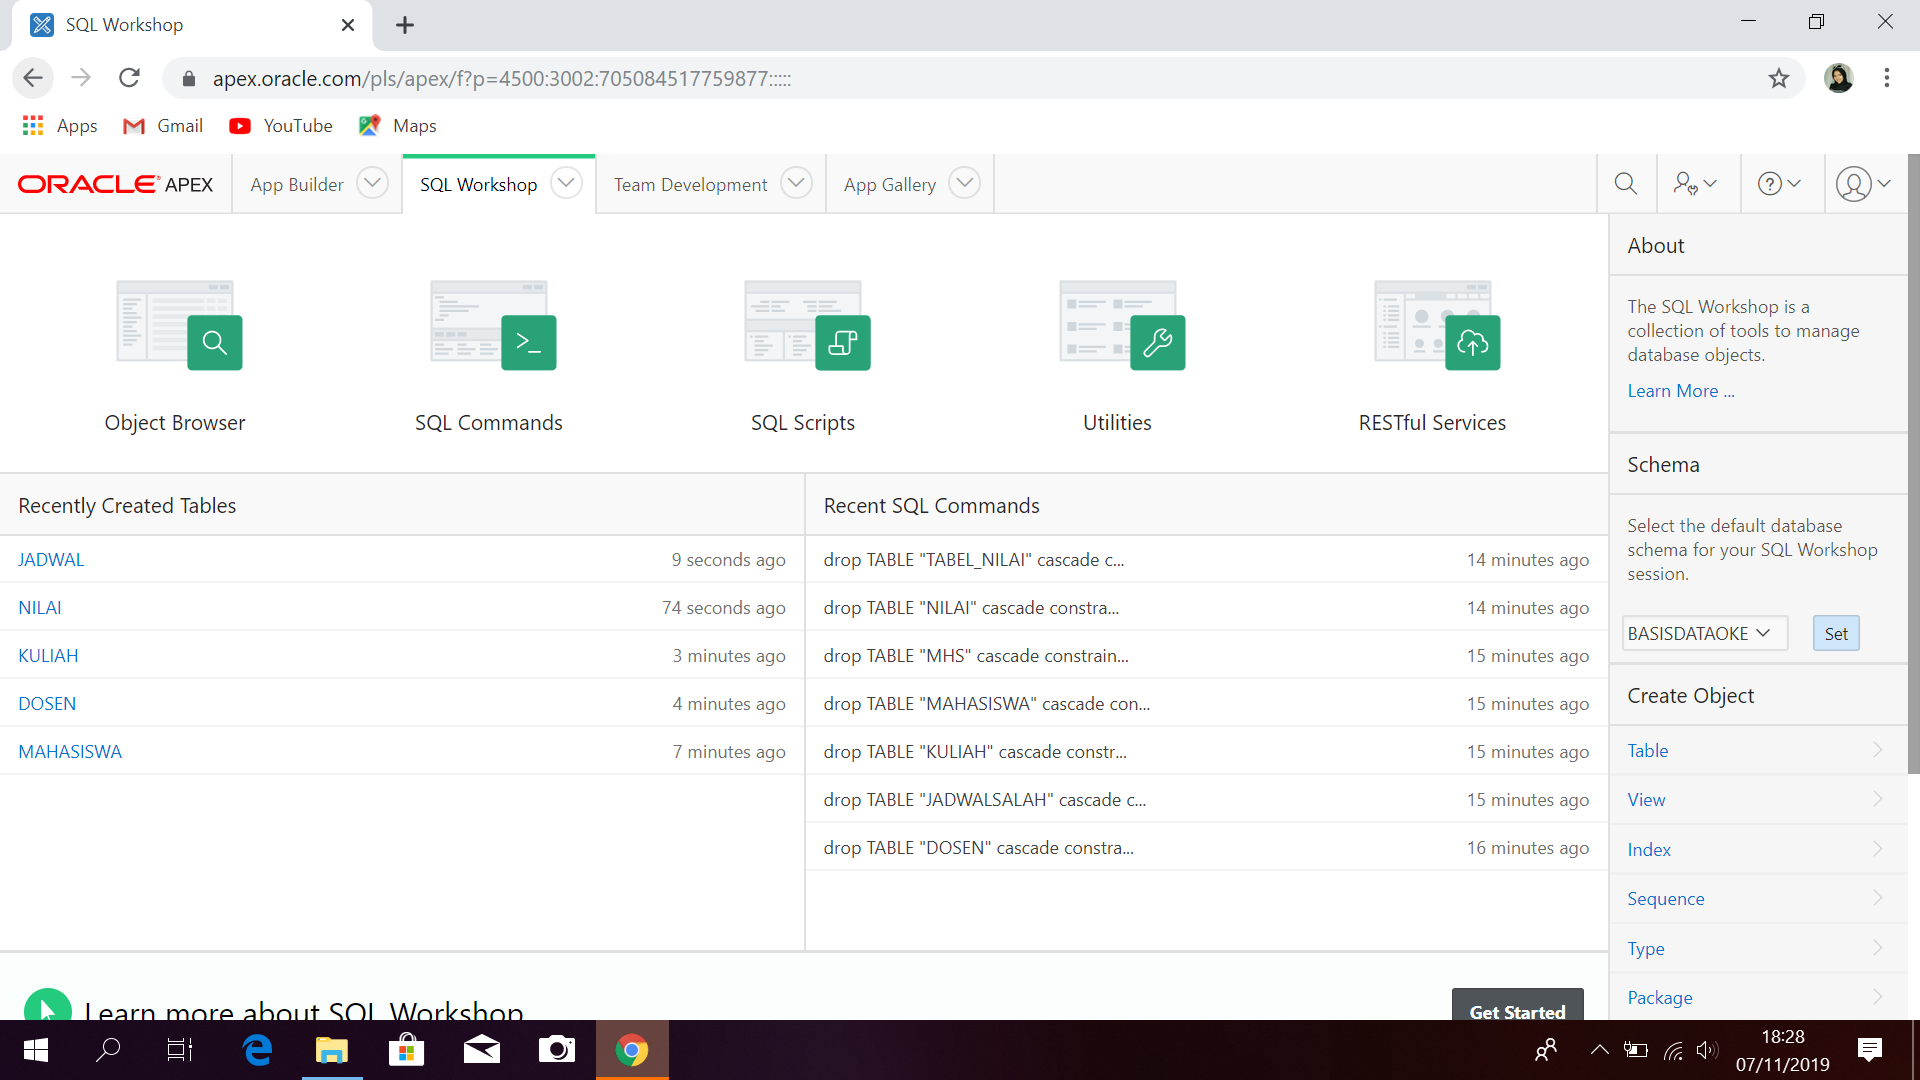
\includegraphics[width=.8\textwidth]{figure/16.PNG}
    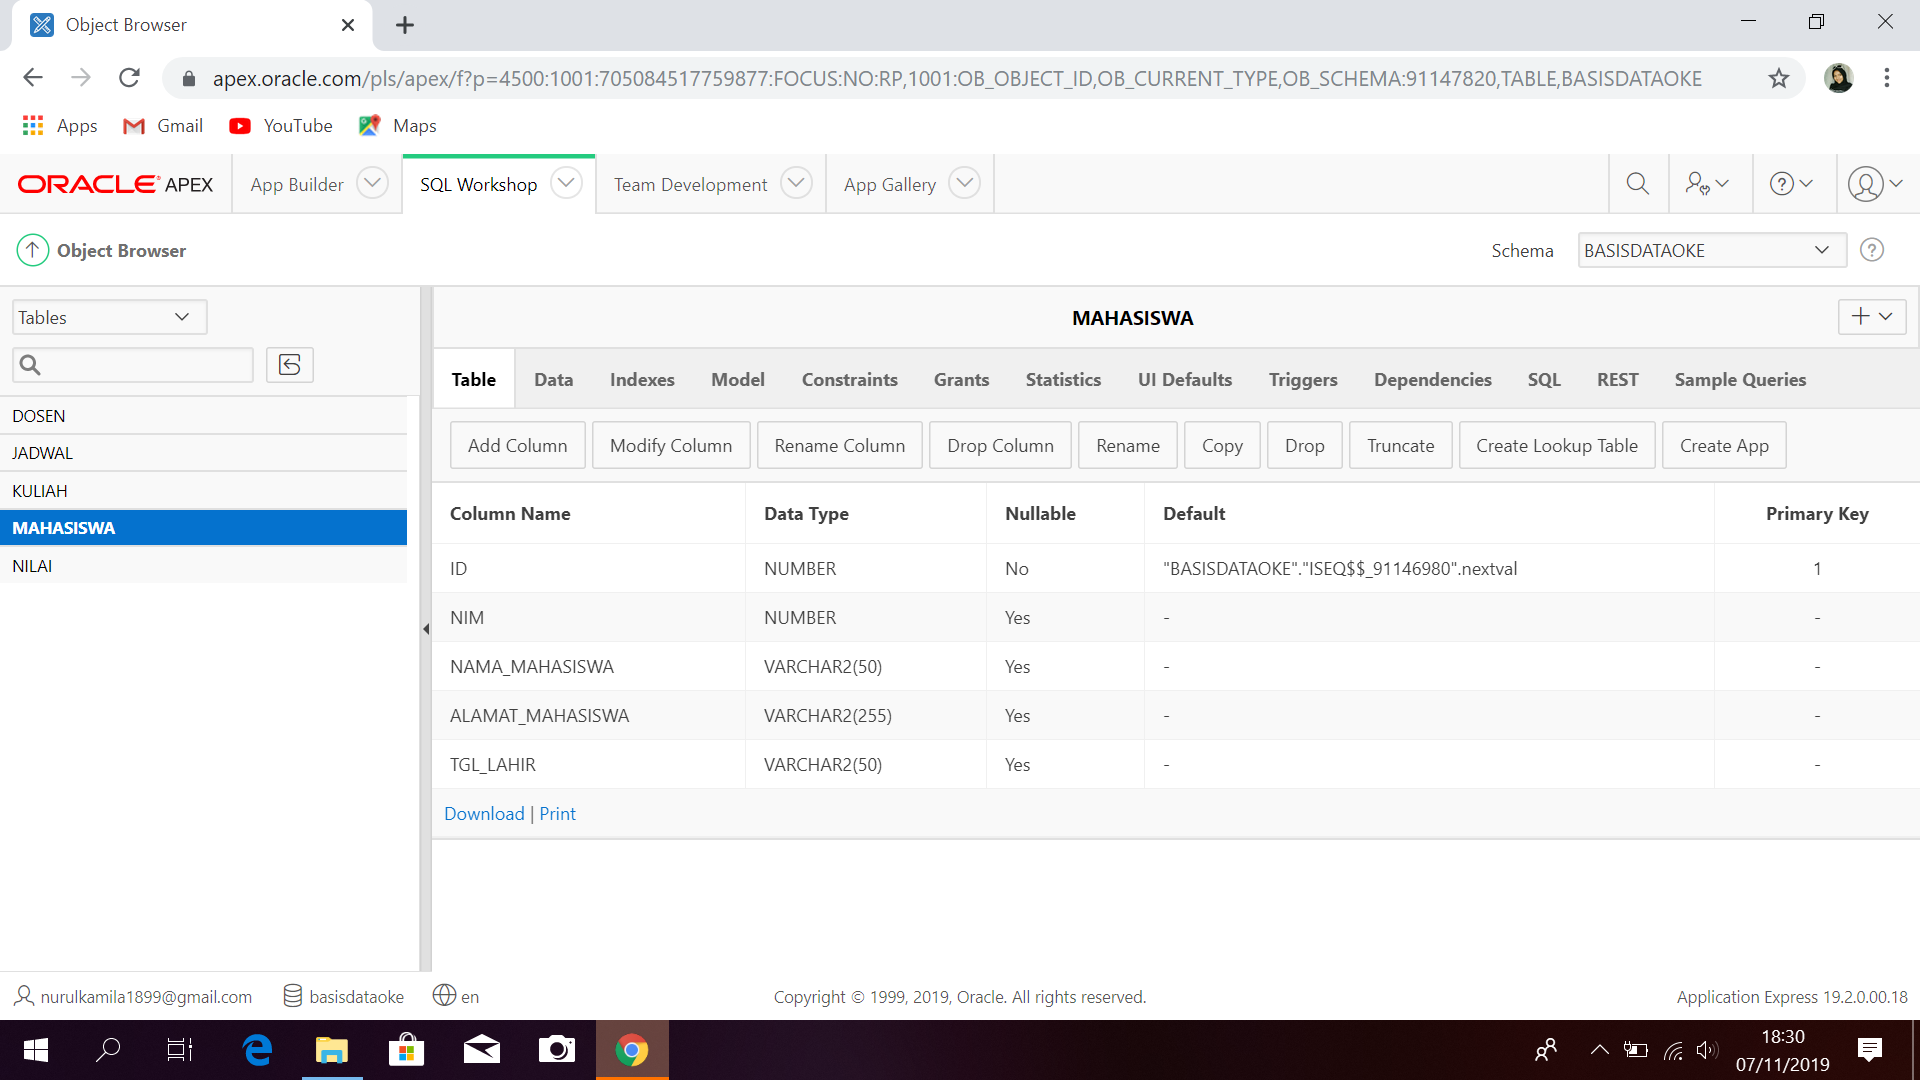
\includegraphics[width=.8\textwidth]{figure/17.PNG}
    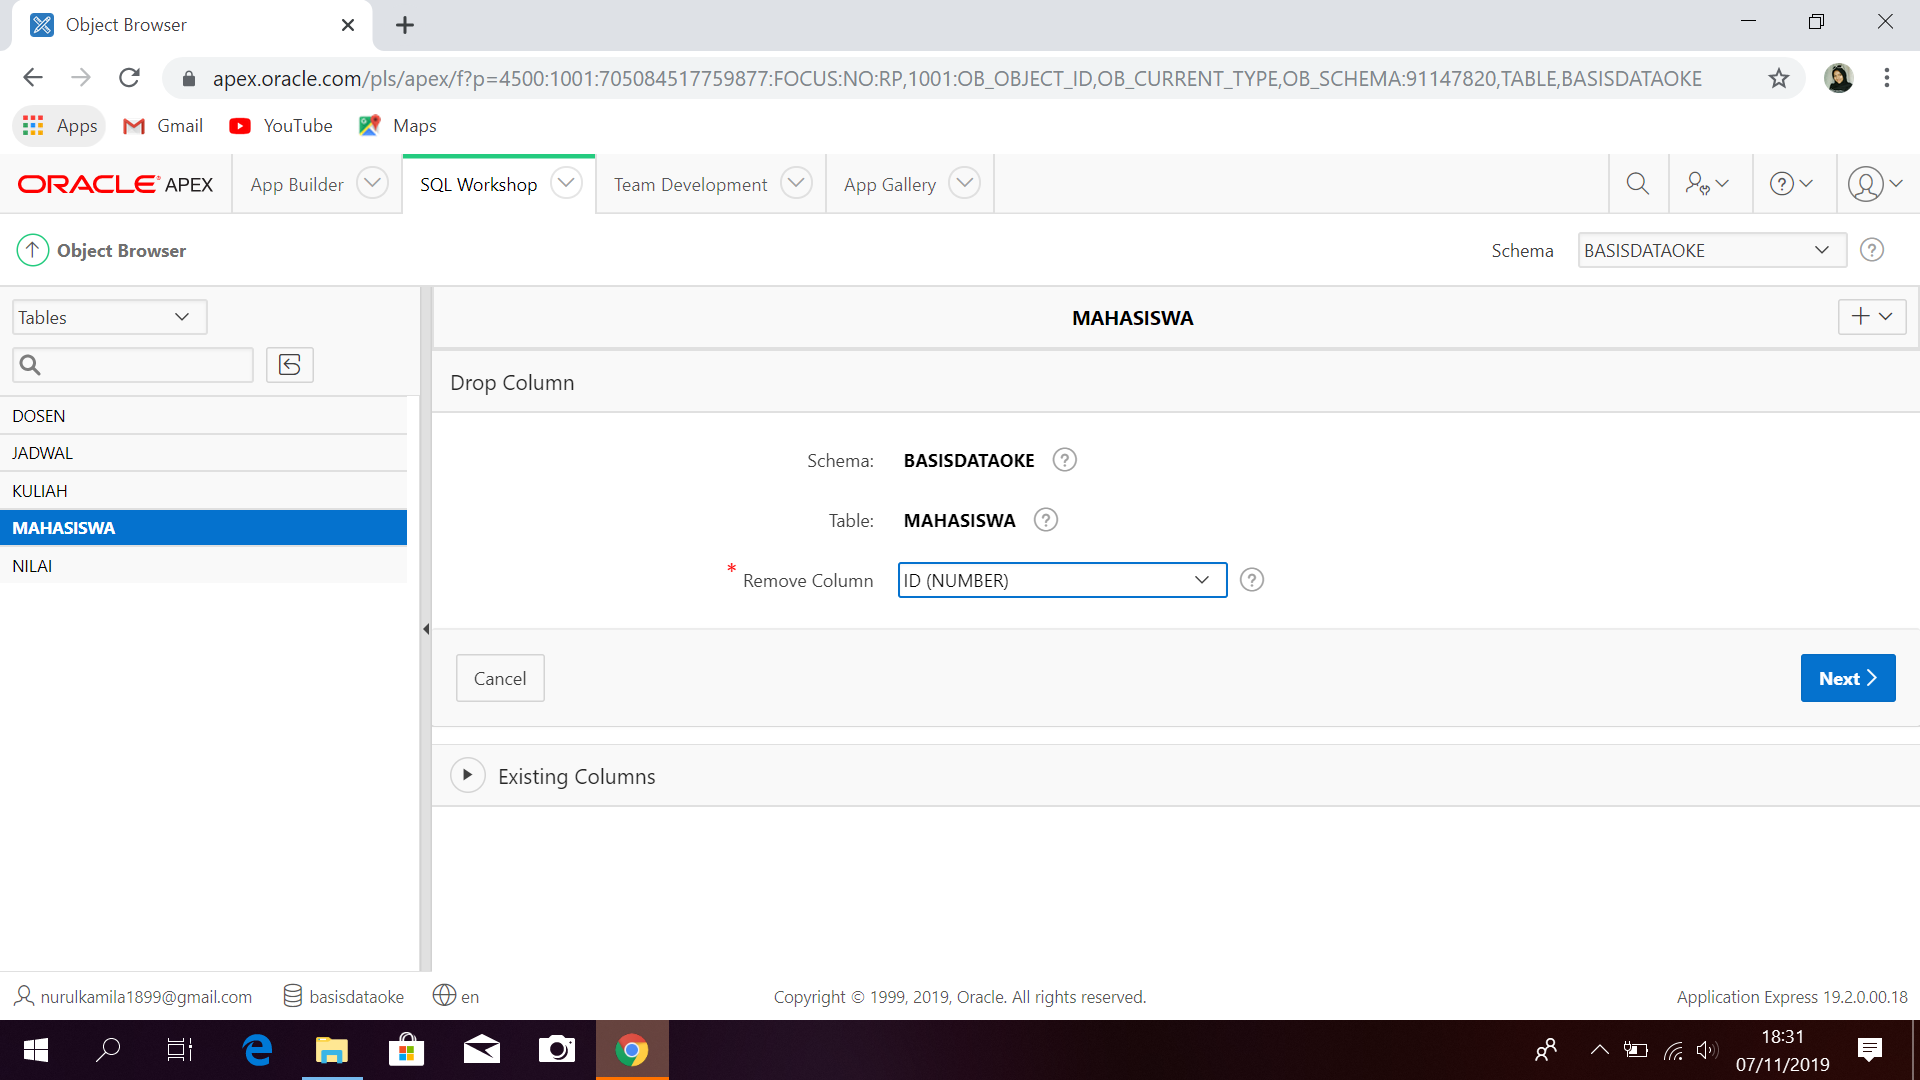
\includegraphics[width=.8\textwidth]{figure/18.PNG}
    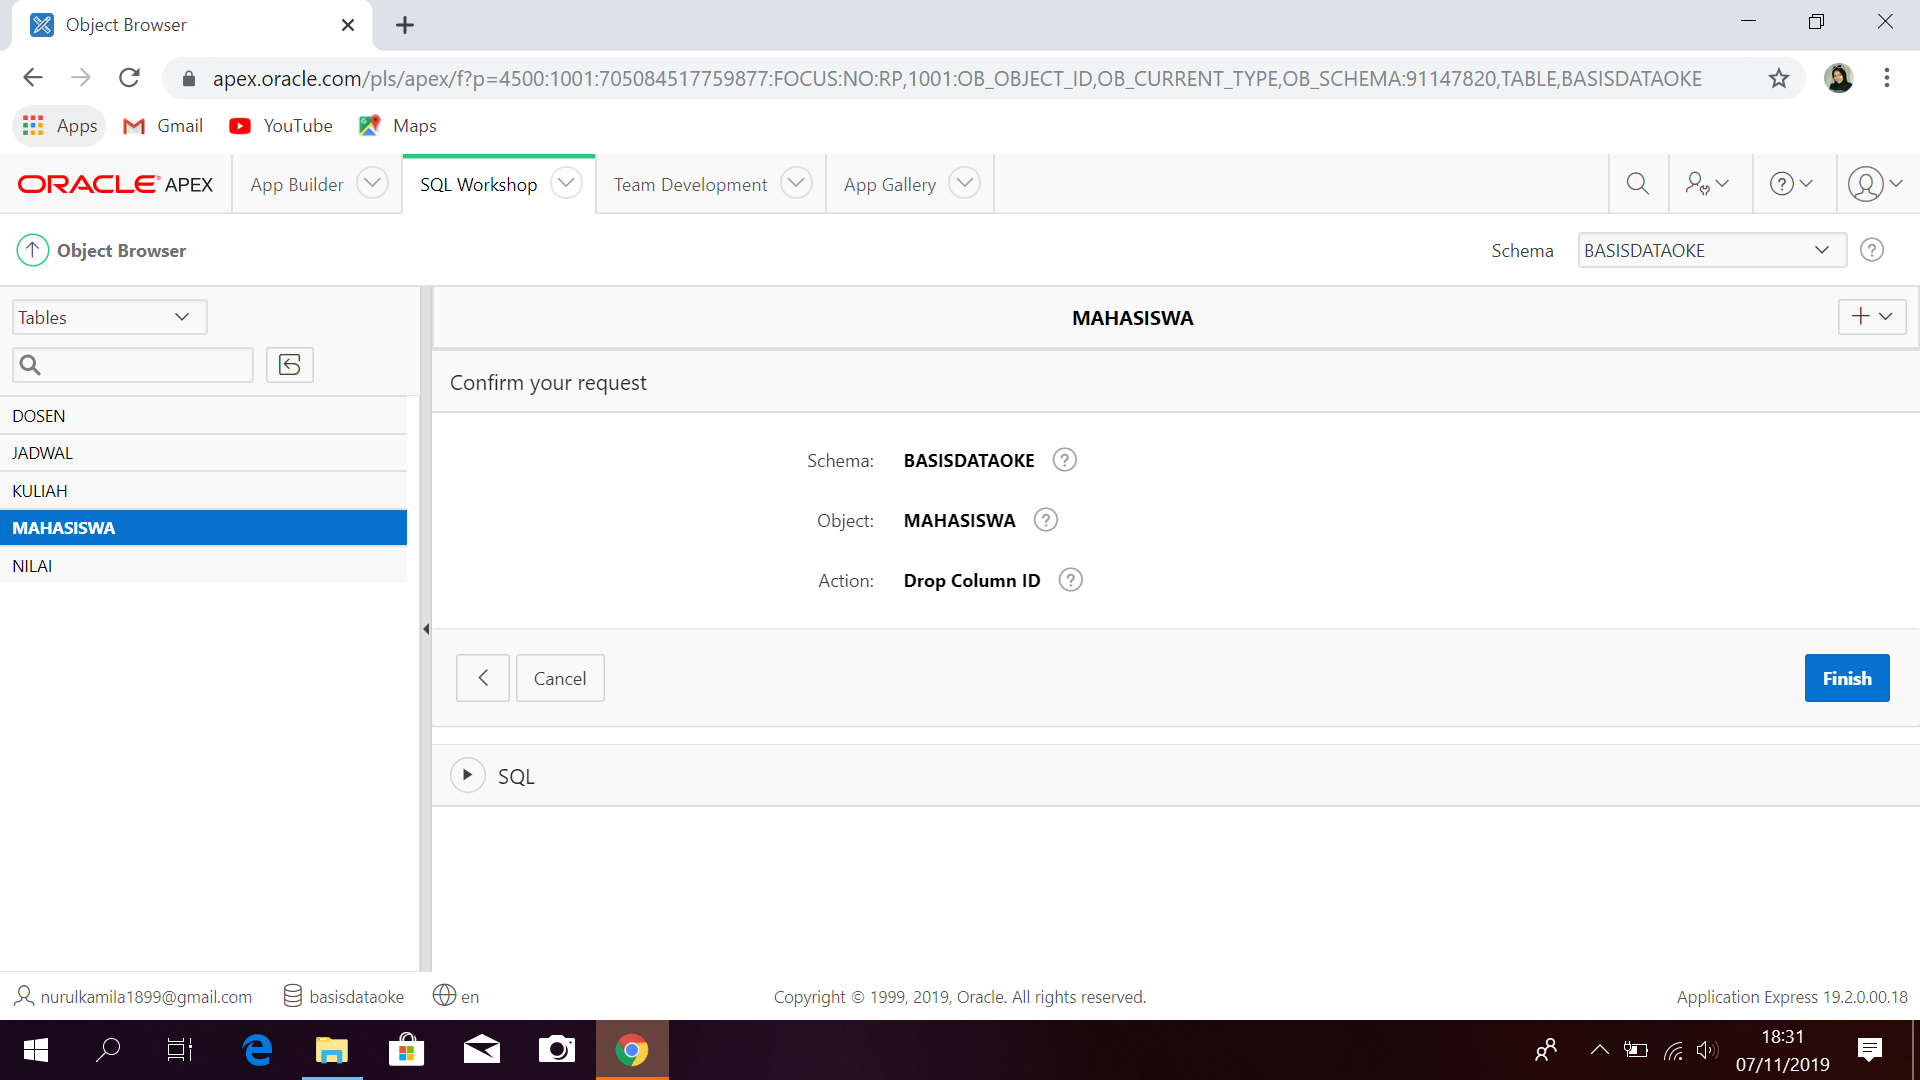
\includegraphics[width=.8\textwidth]{figure/19.PNG}
    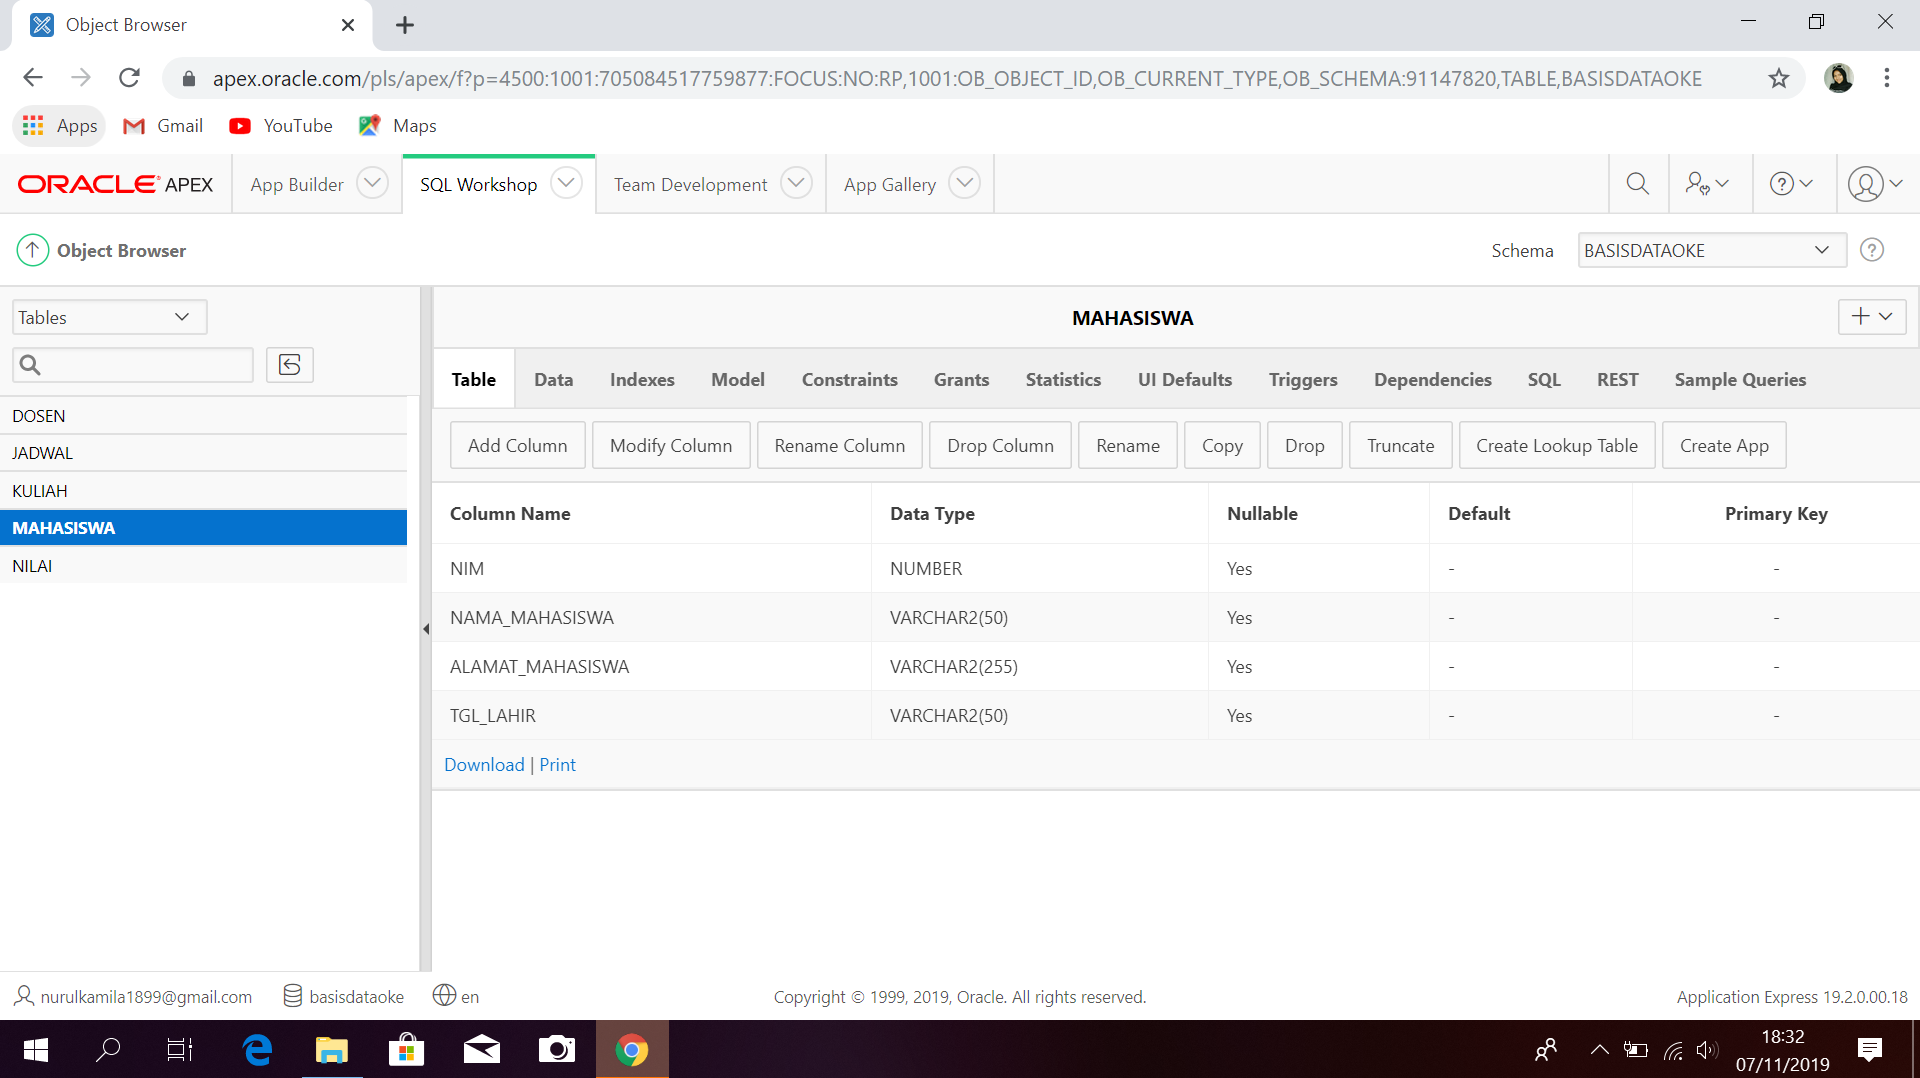
\includegraphics[width=.8\textwidth]{figure/20.PNG}
    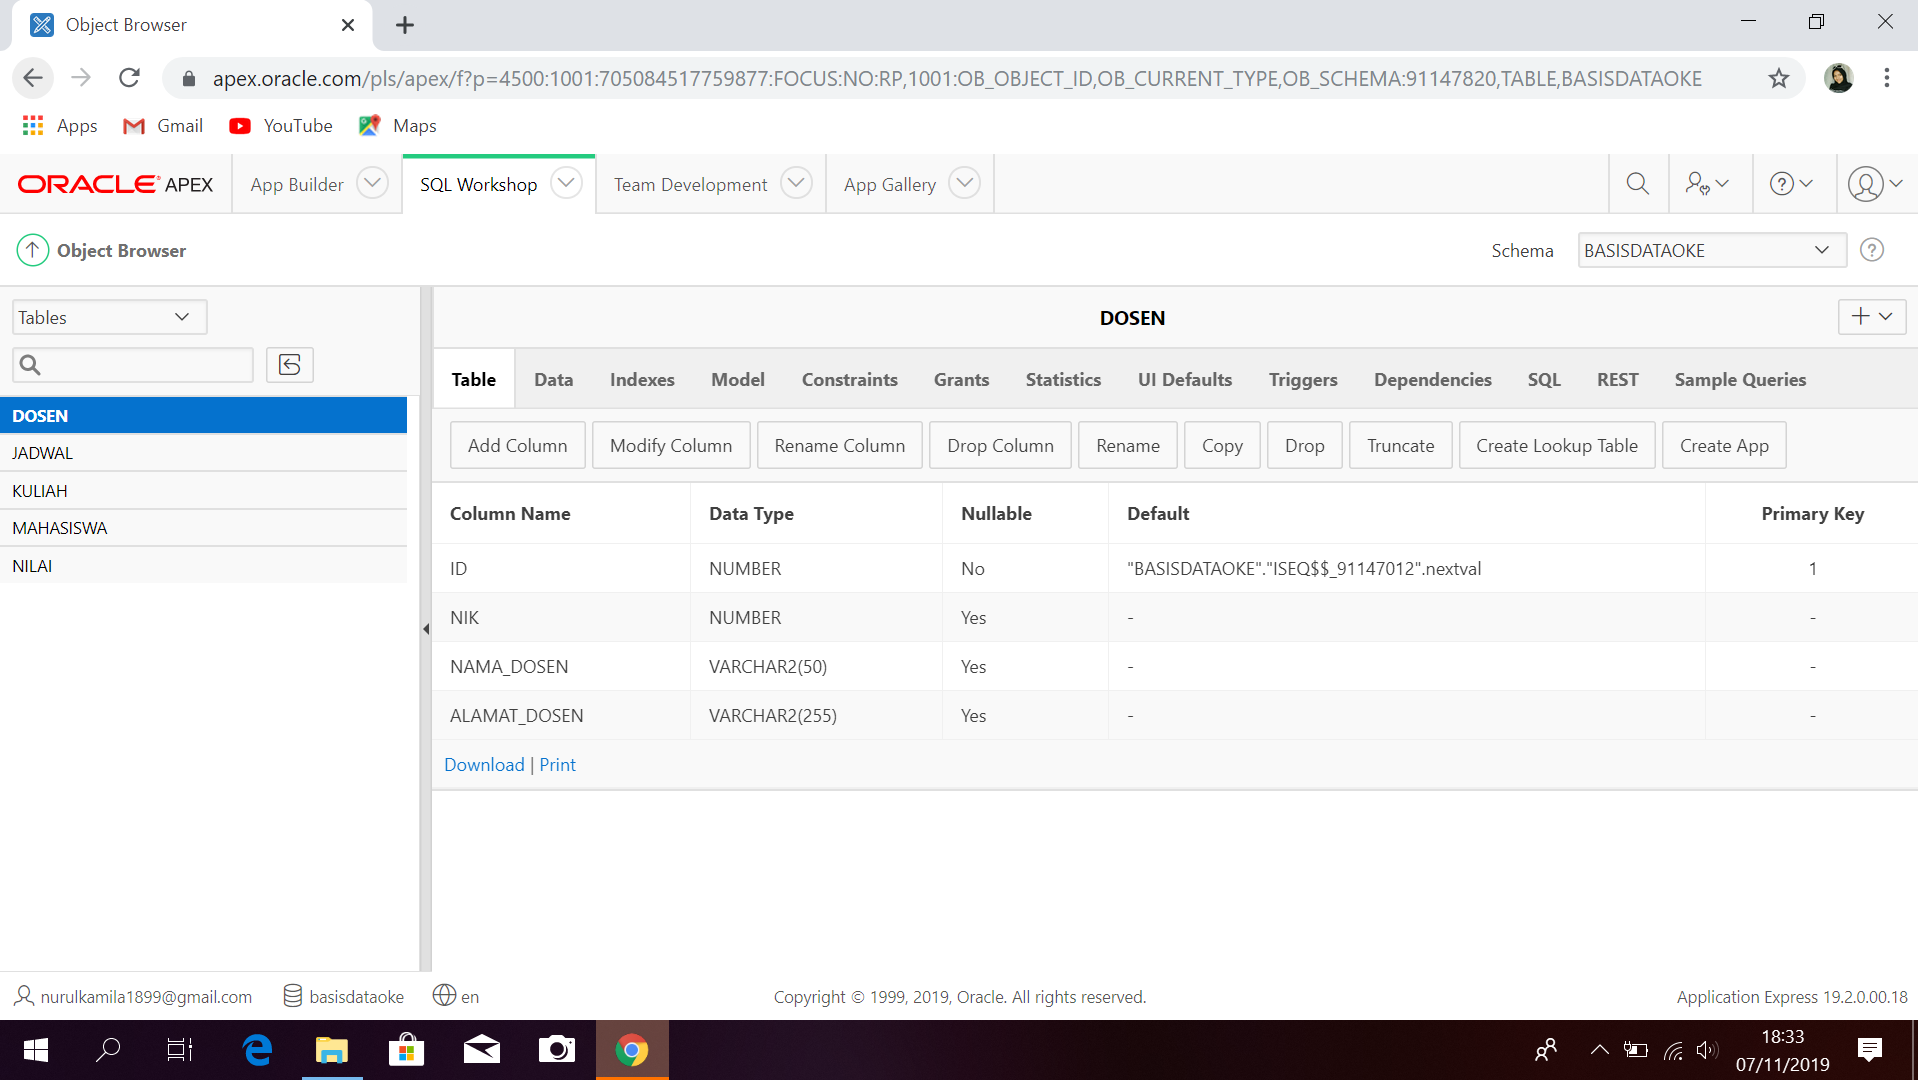
\includegraphics[width=.8\textwidth]{figure/21.PNG}
    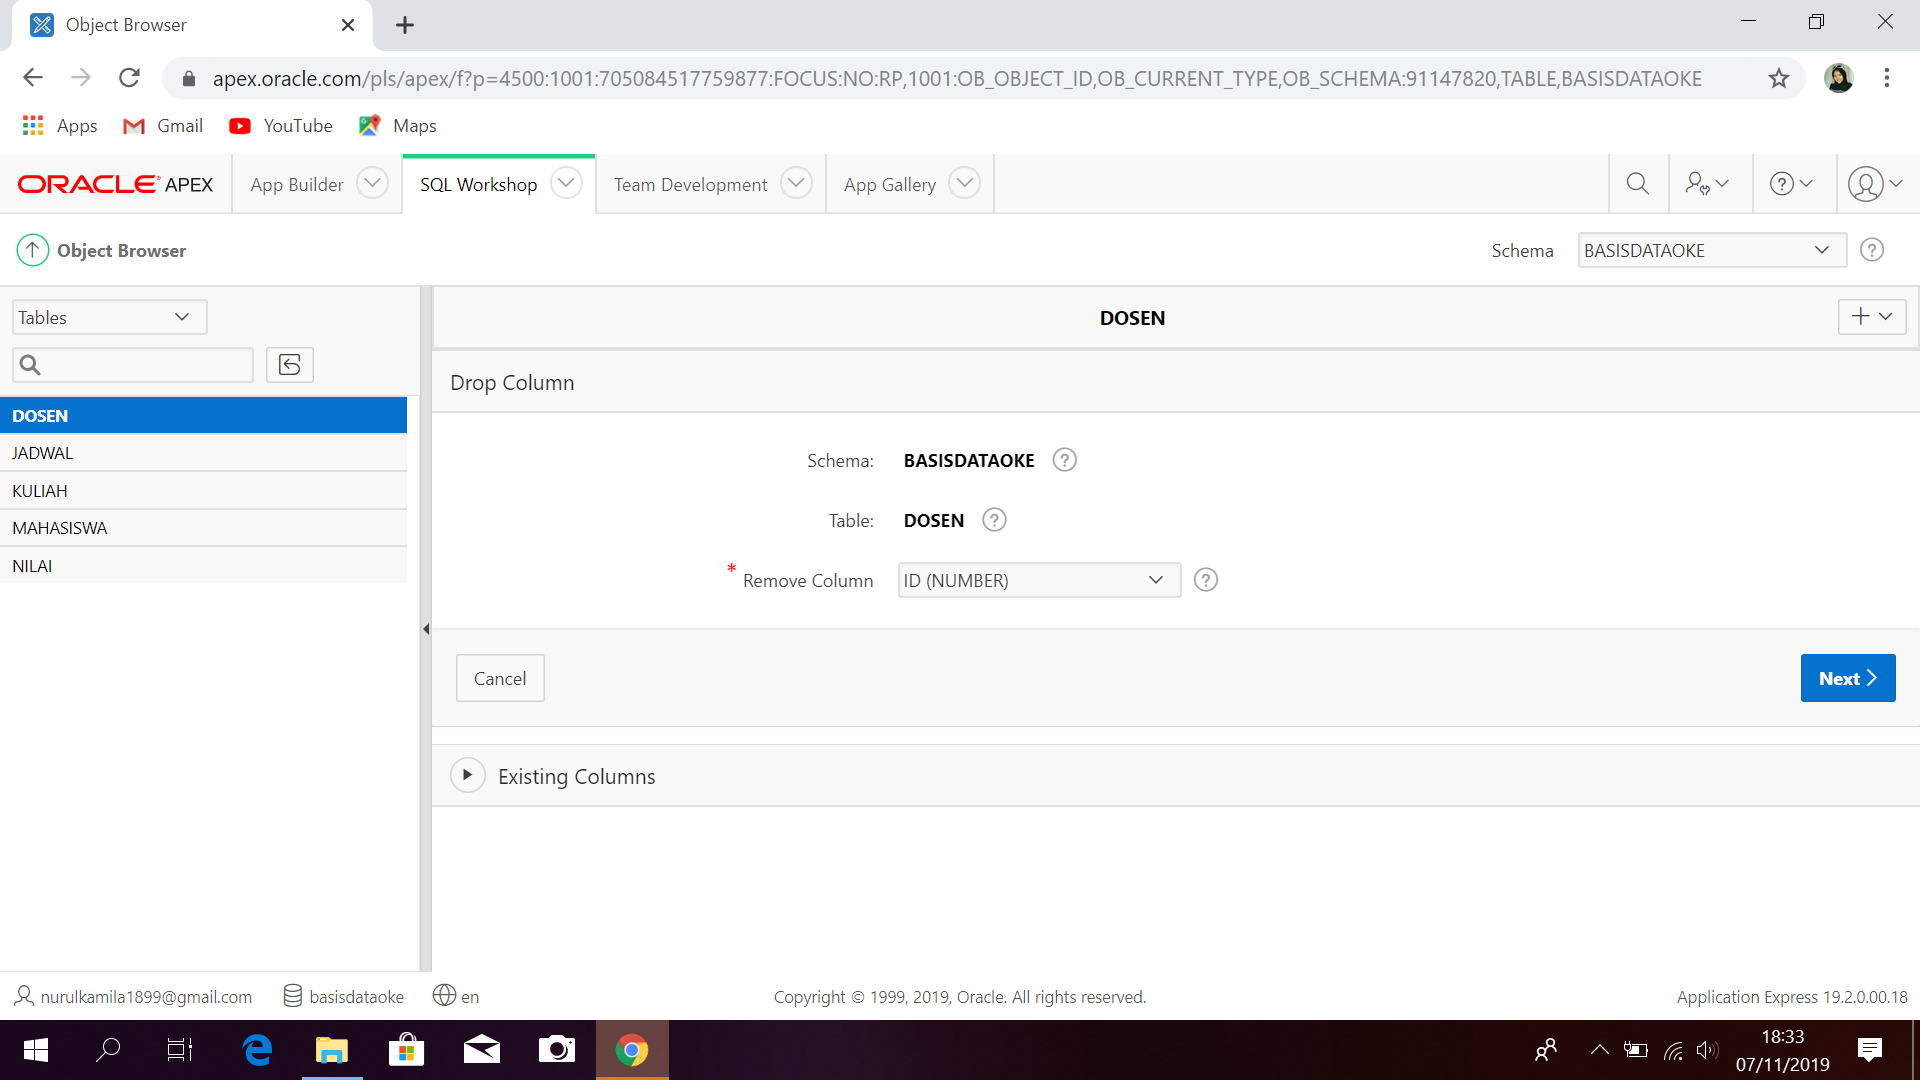
\includegraphics[width=.8\textwidth]{figure/22.PNG}
    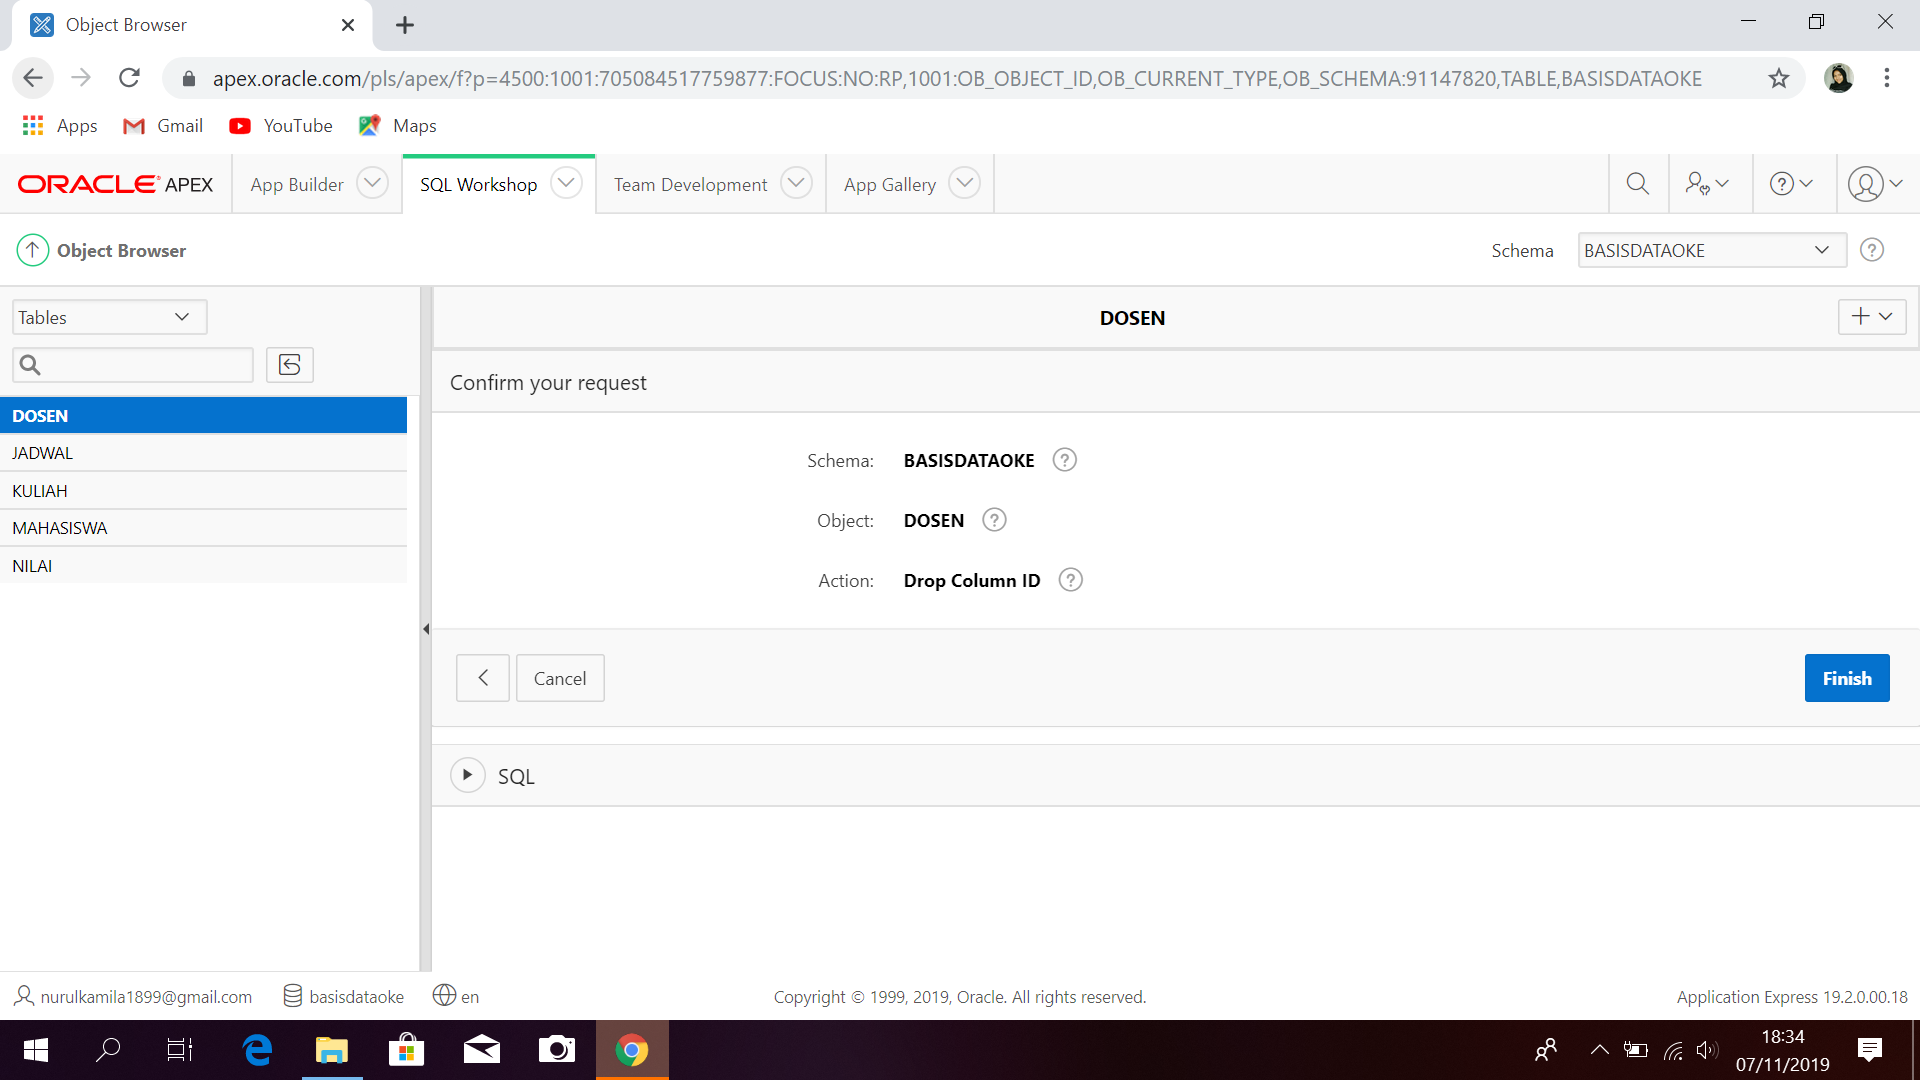
\includegraphics[width=.8\textwidth]{figure/23.PNG}
    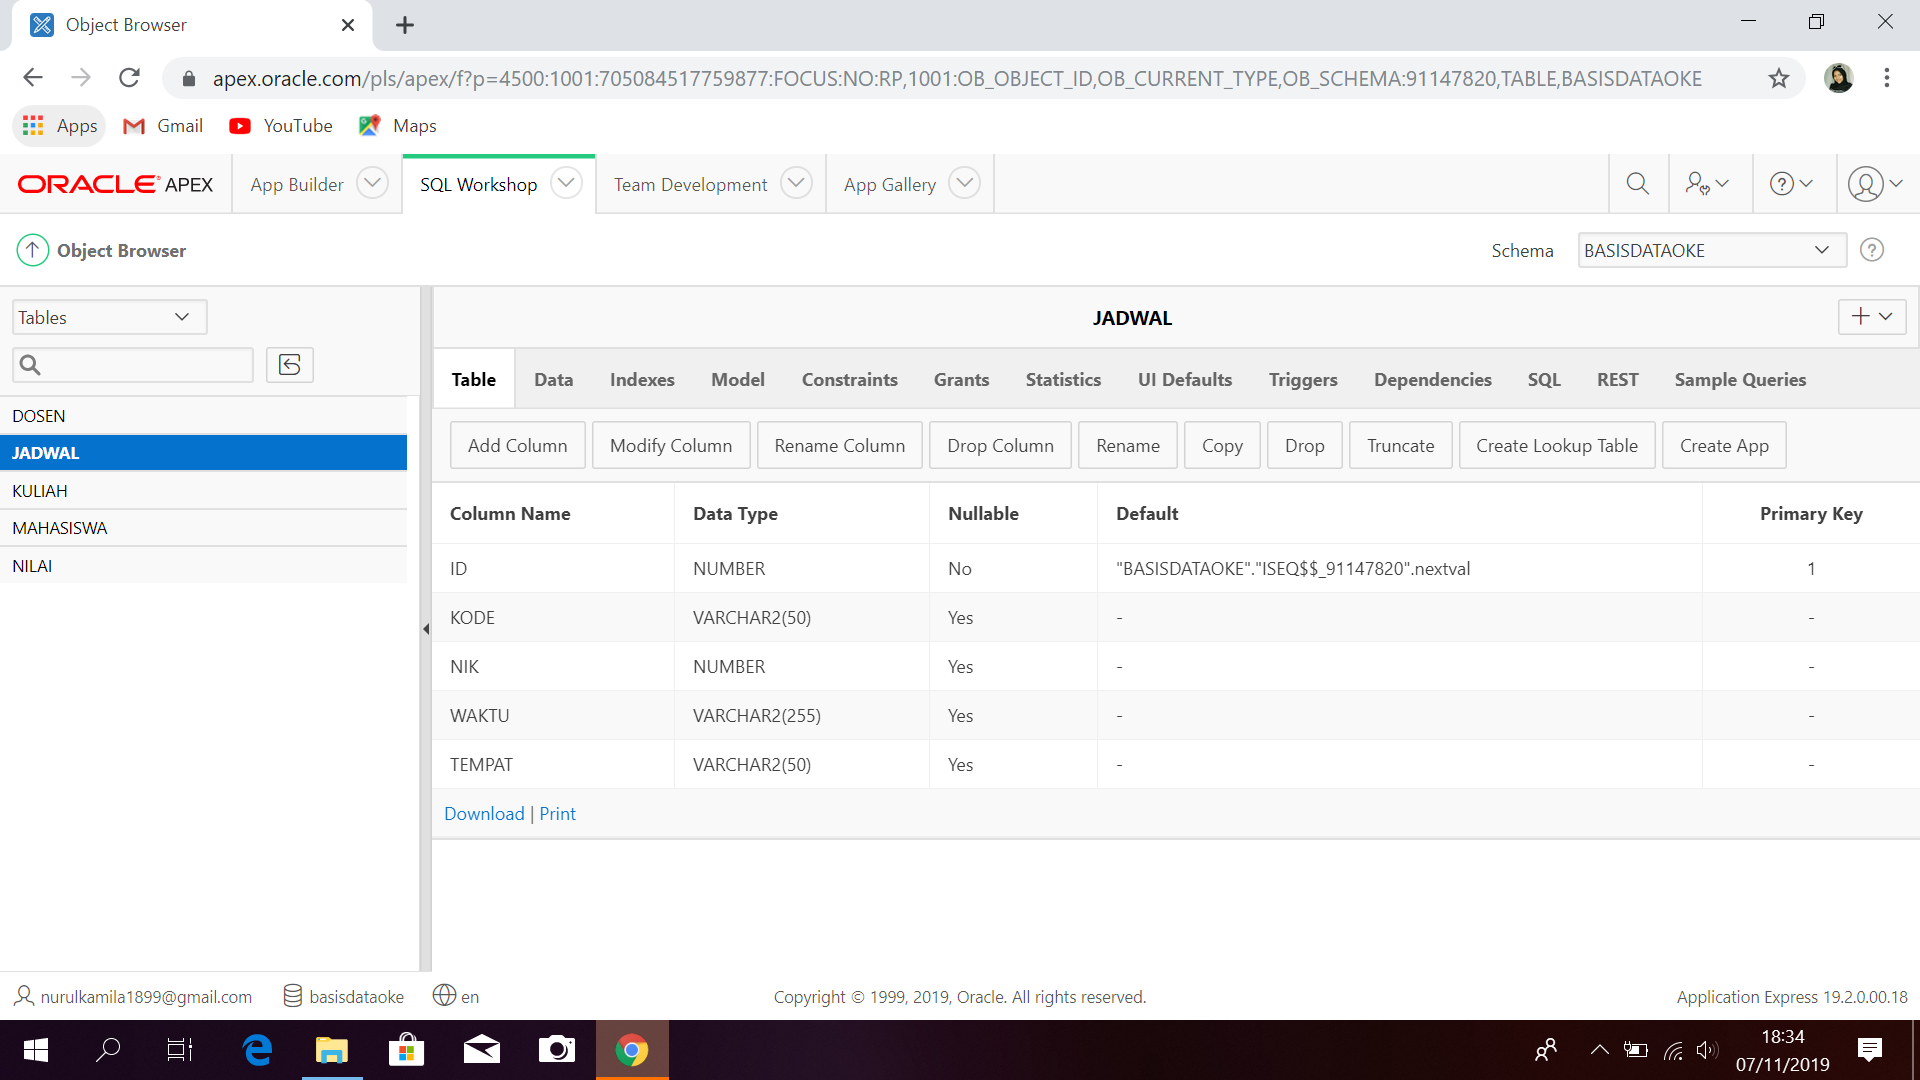
\includegraphics[width=.8\textwidth]{figure/24.PNG}
    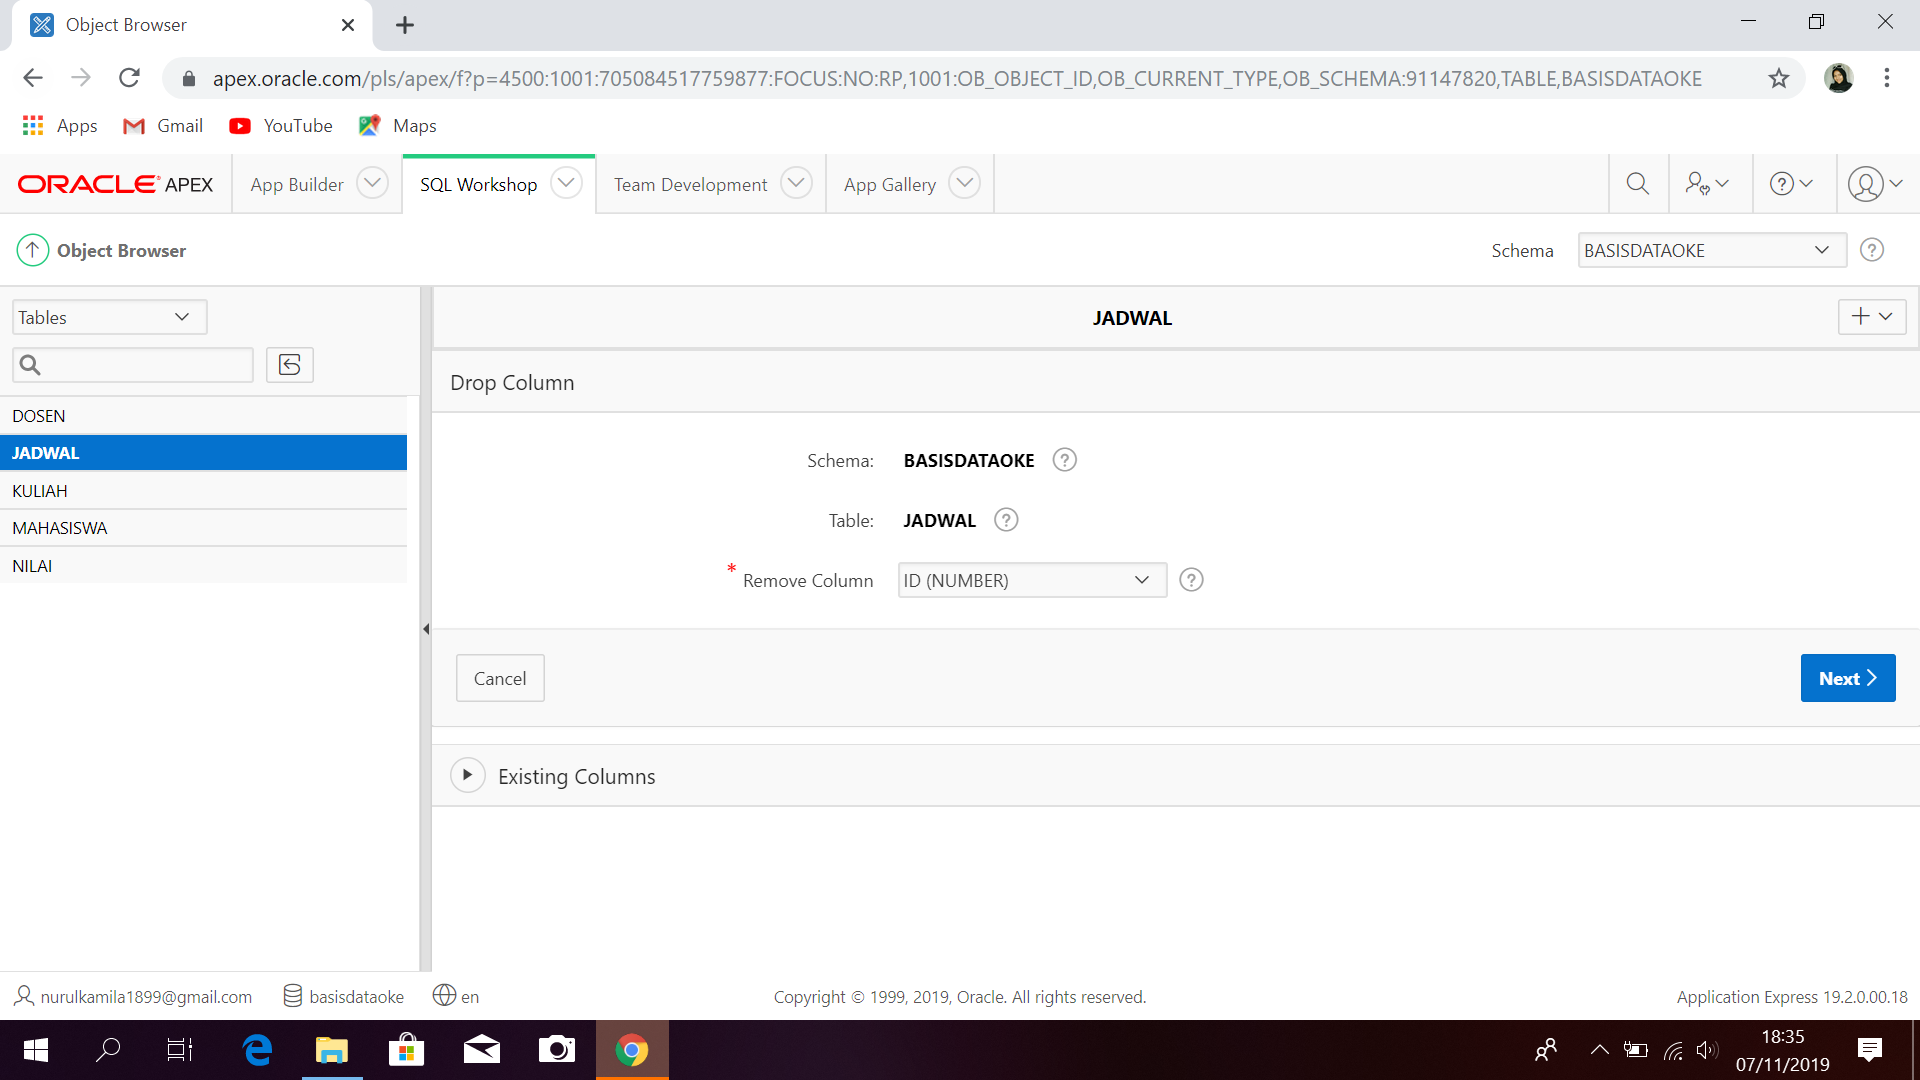
\includegraphics[width=.8\textwidth]{figure/25.PNG}
    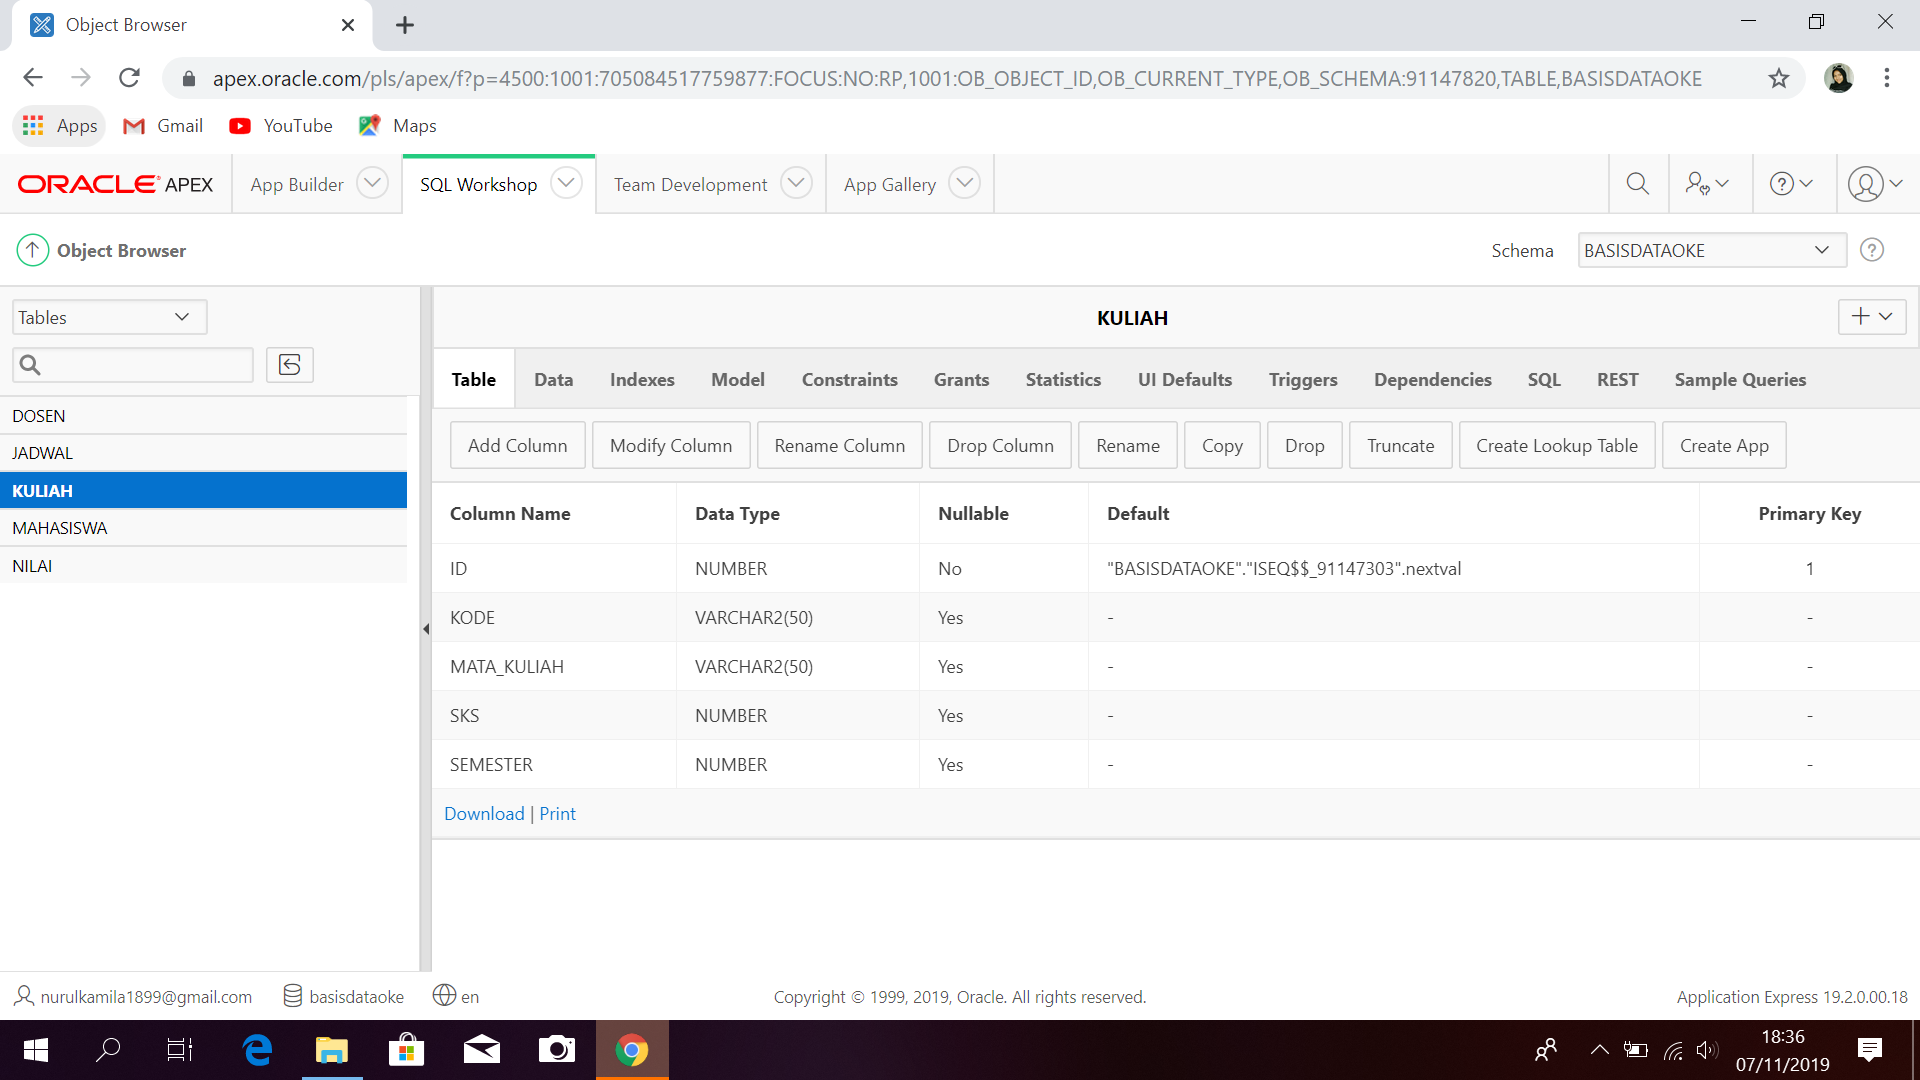
\includegraphics[width=.8\textwidth]{figure/26.PNG}
    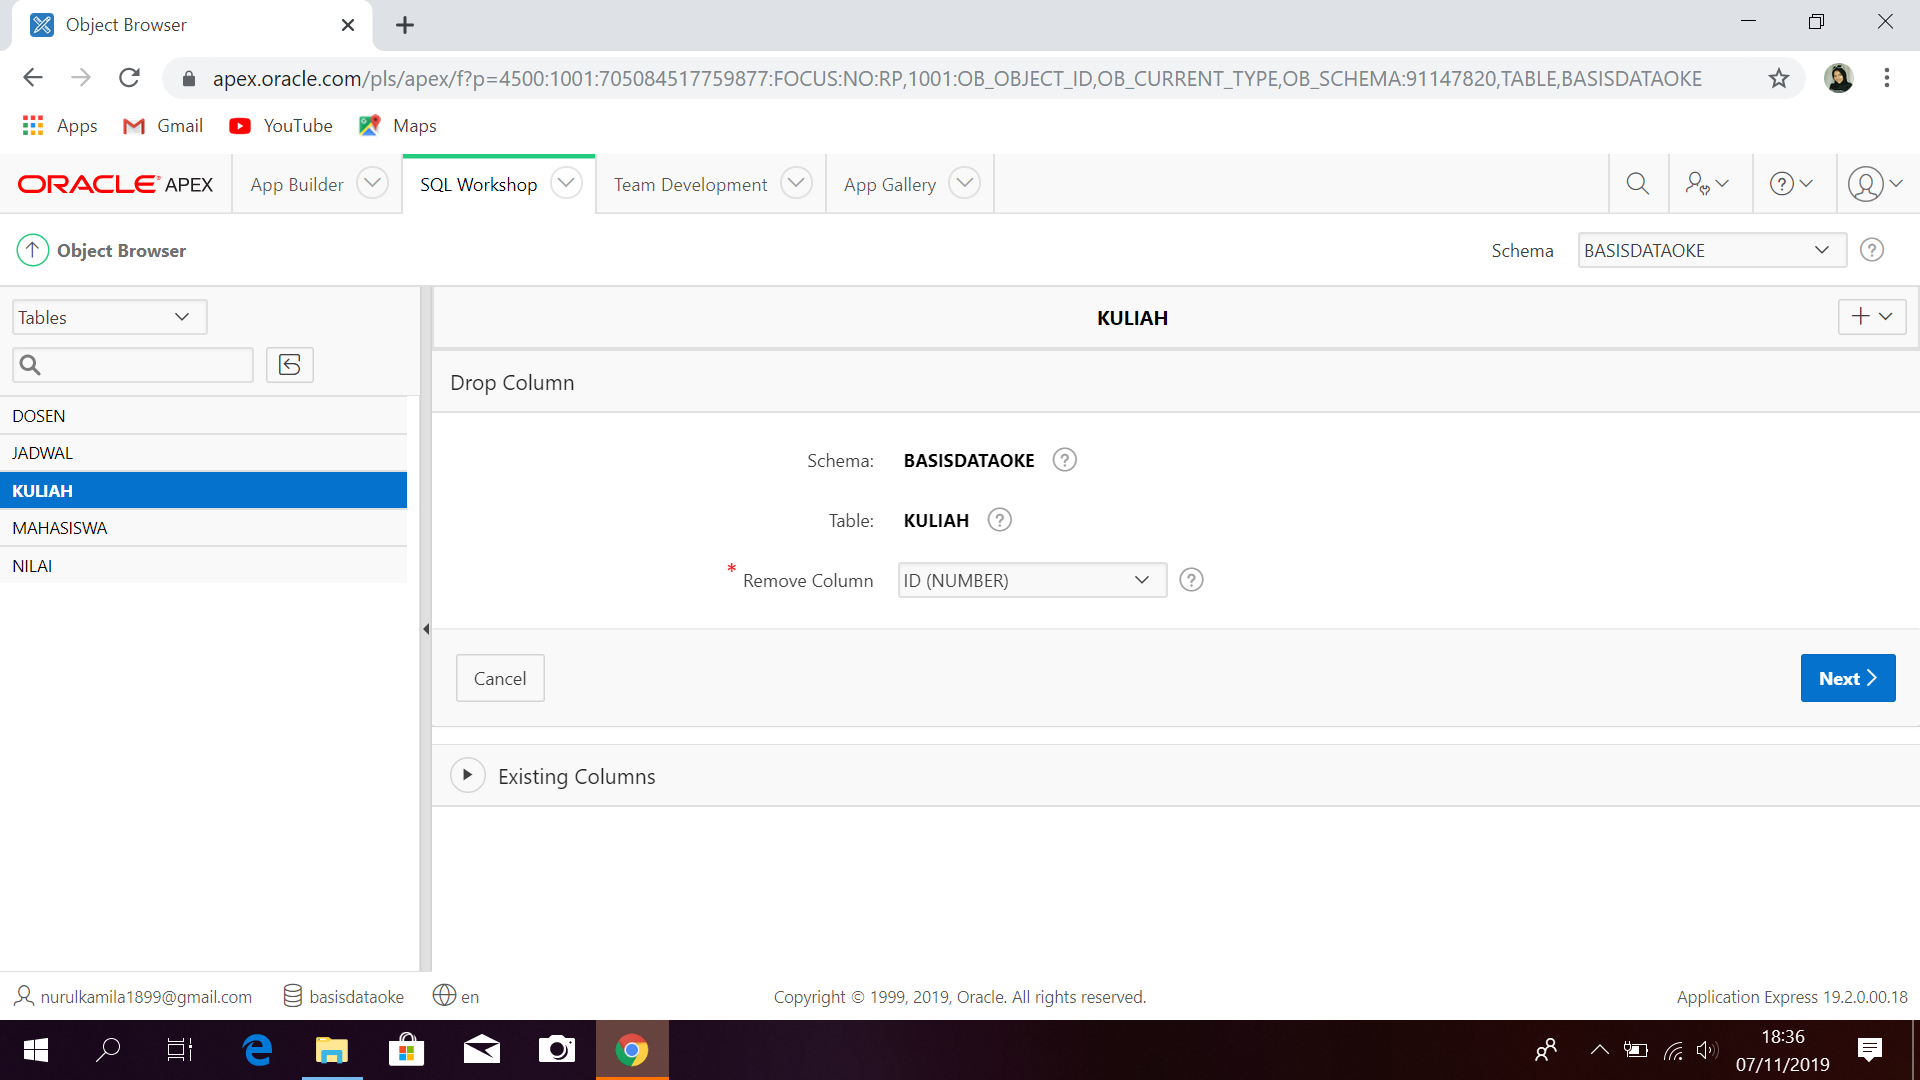
\includegraphics[width=.8\textwidth]{figure/27.PNG}
    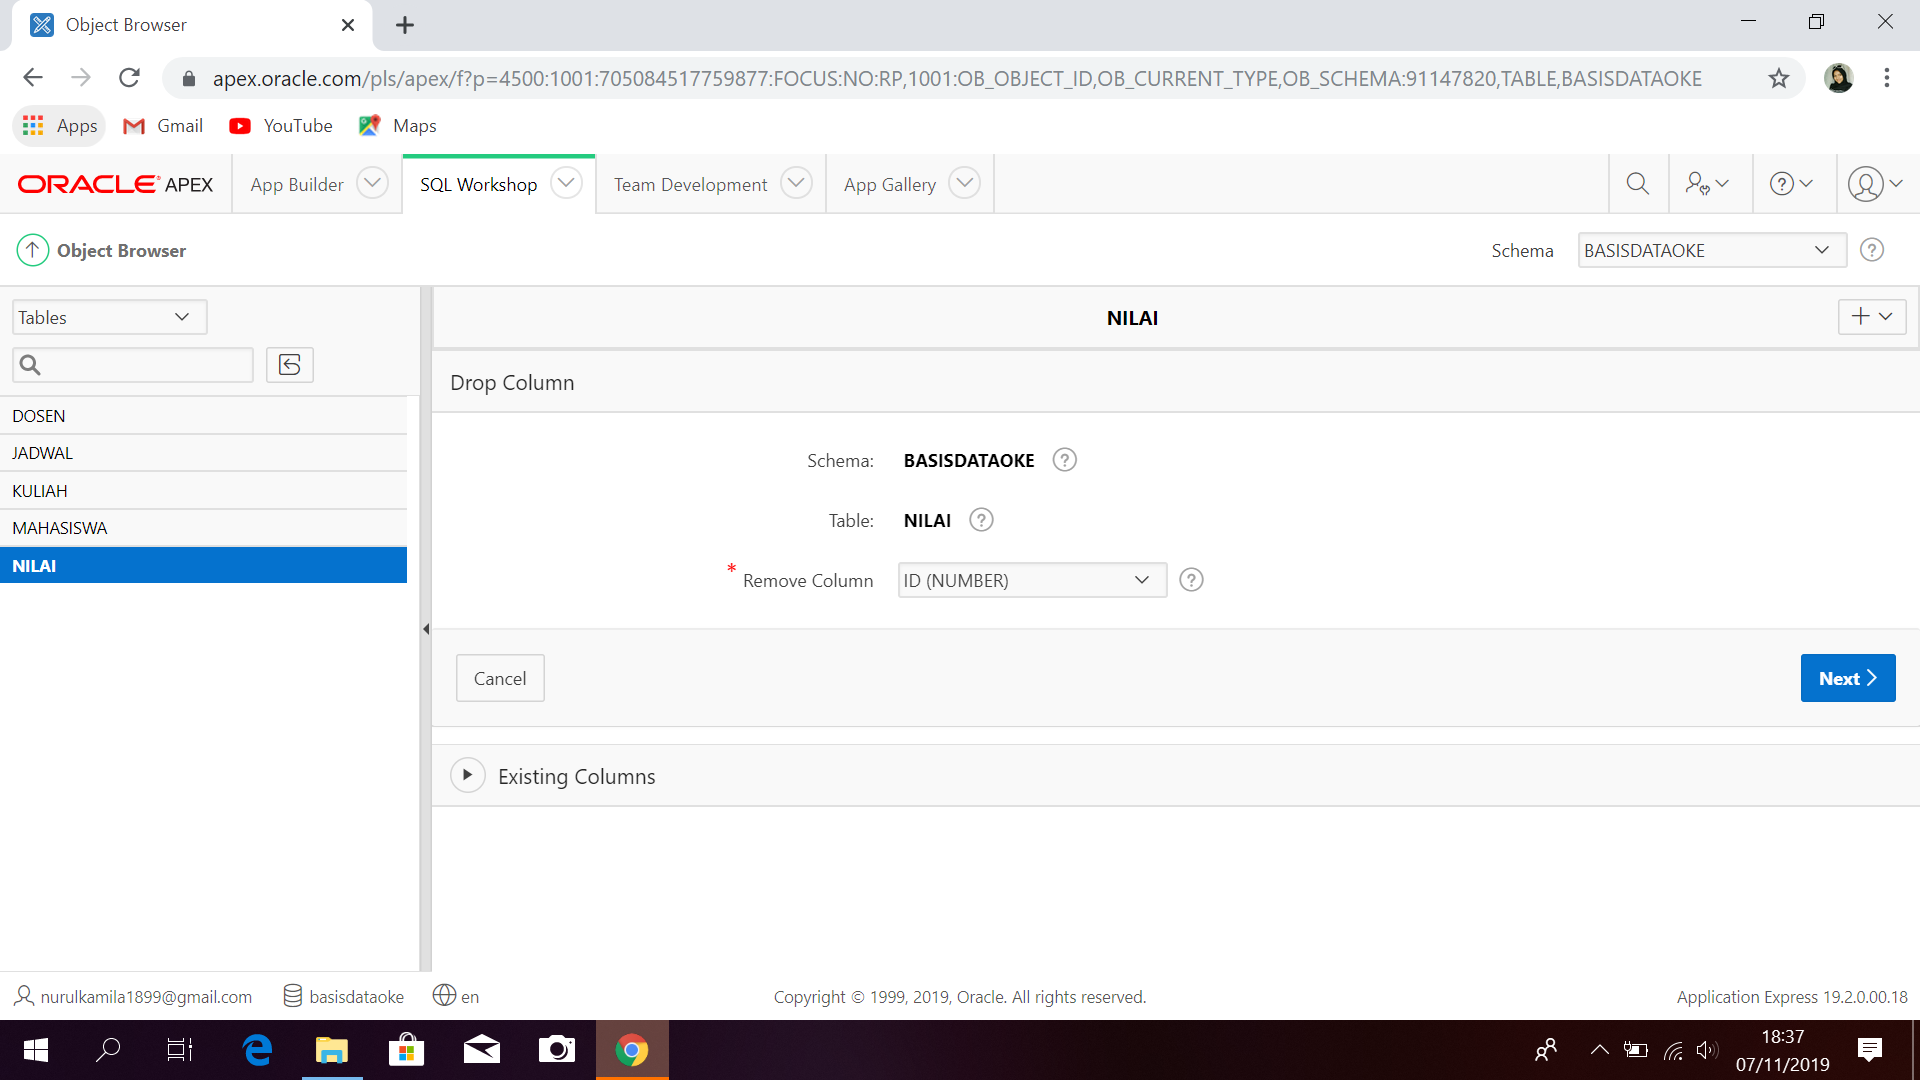
\includegraphics[width=.8\textwidth]{figure/29.PNG}
    \end{center}
    \item setelah itu, pada pilihan constrains, setting primery key, dan foregent key sesuai tabel 
    \begin{center}
    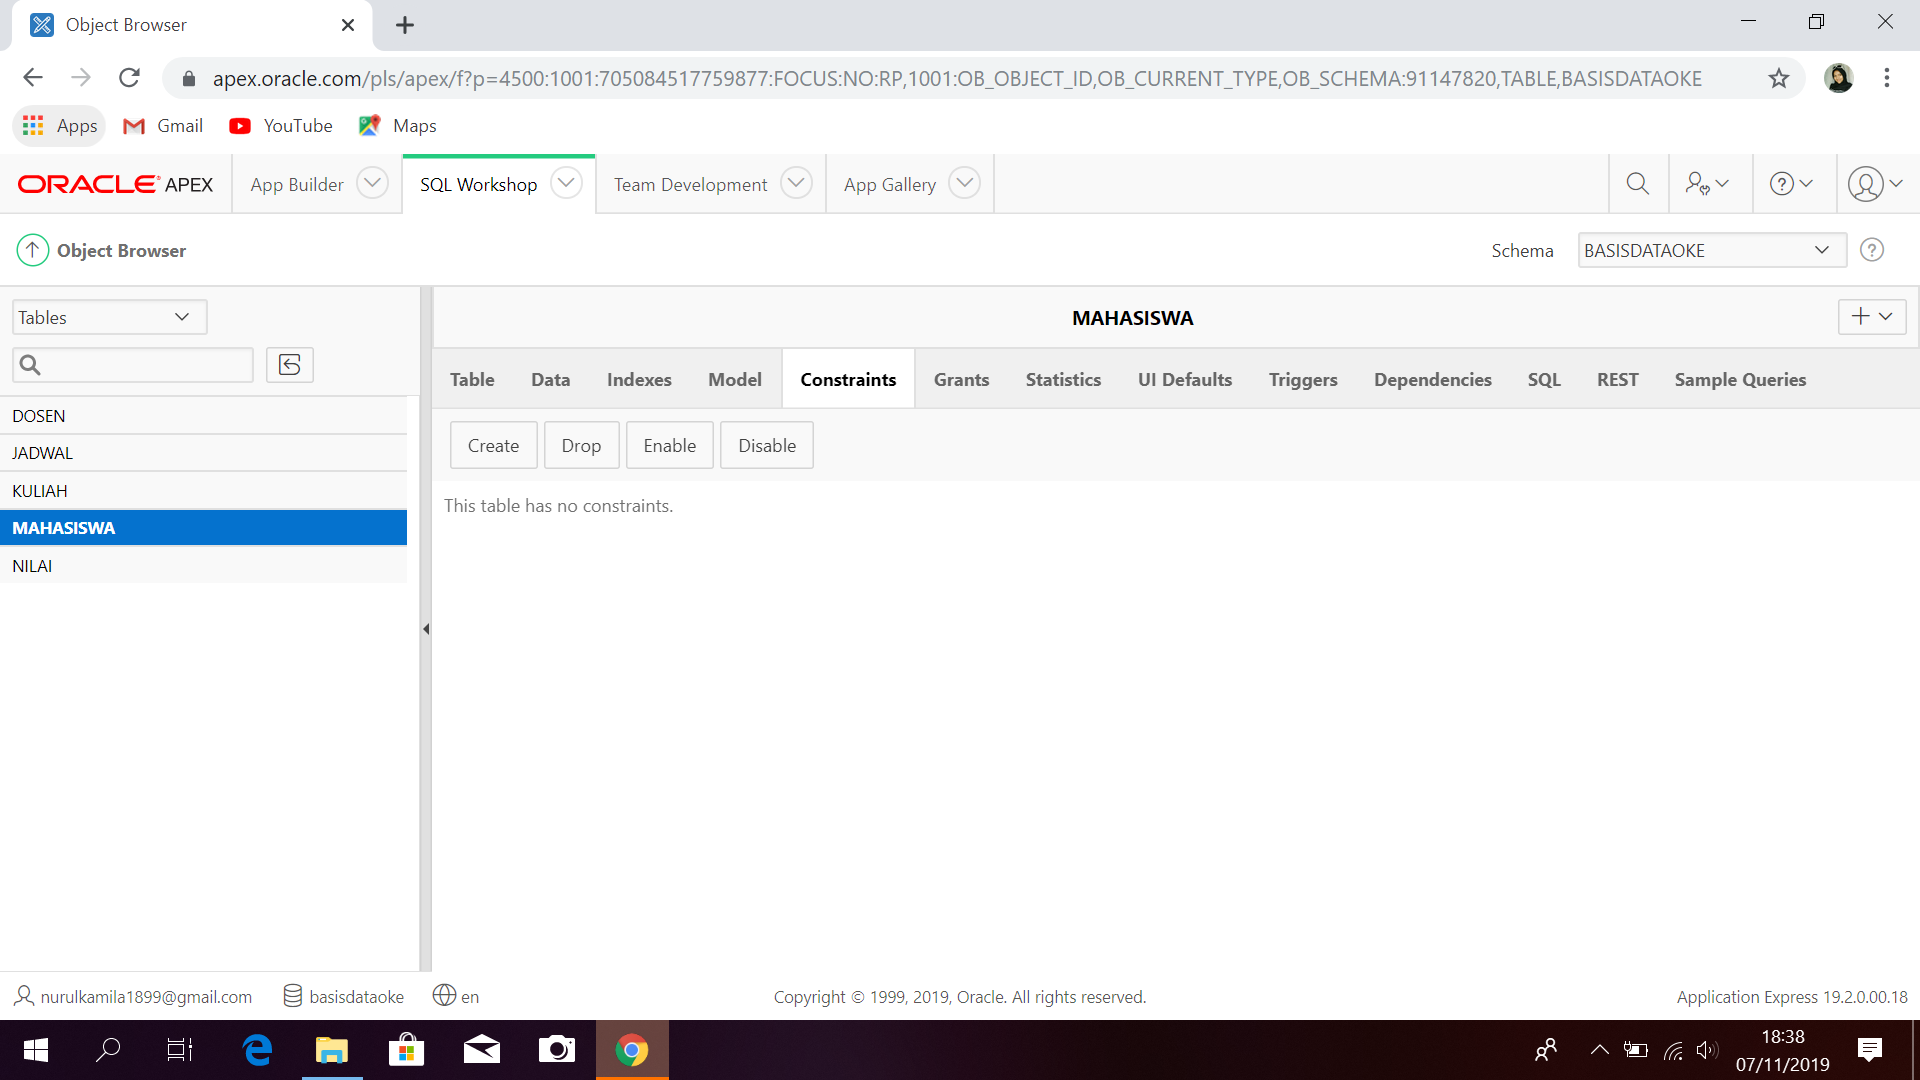
\includegraphics[width=.8\textwidth]{figure/30.PNG}
    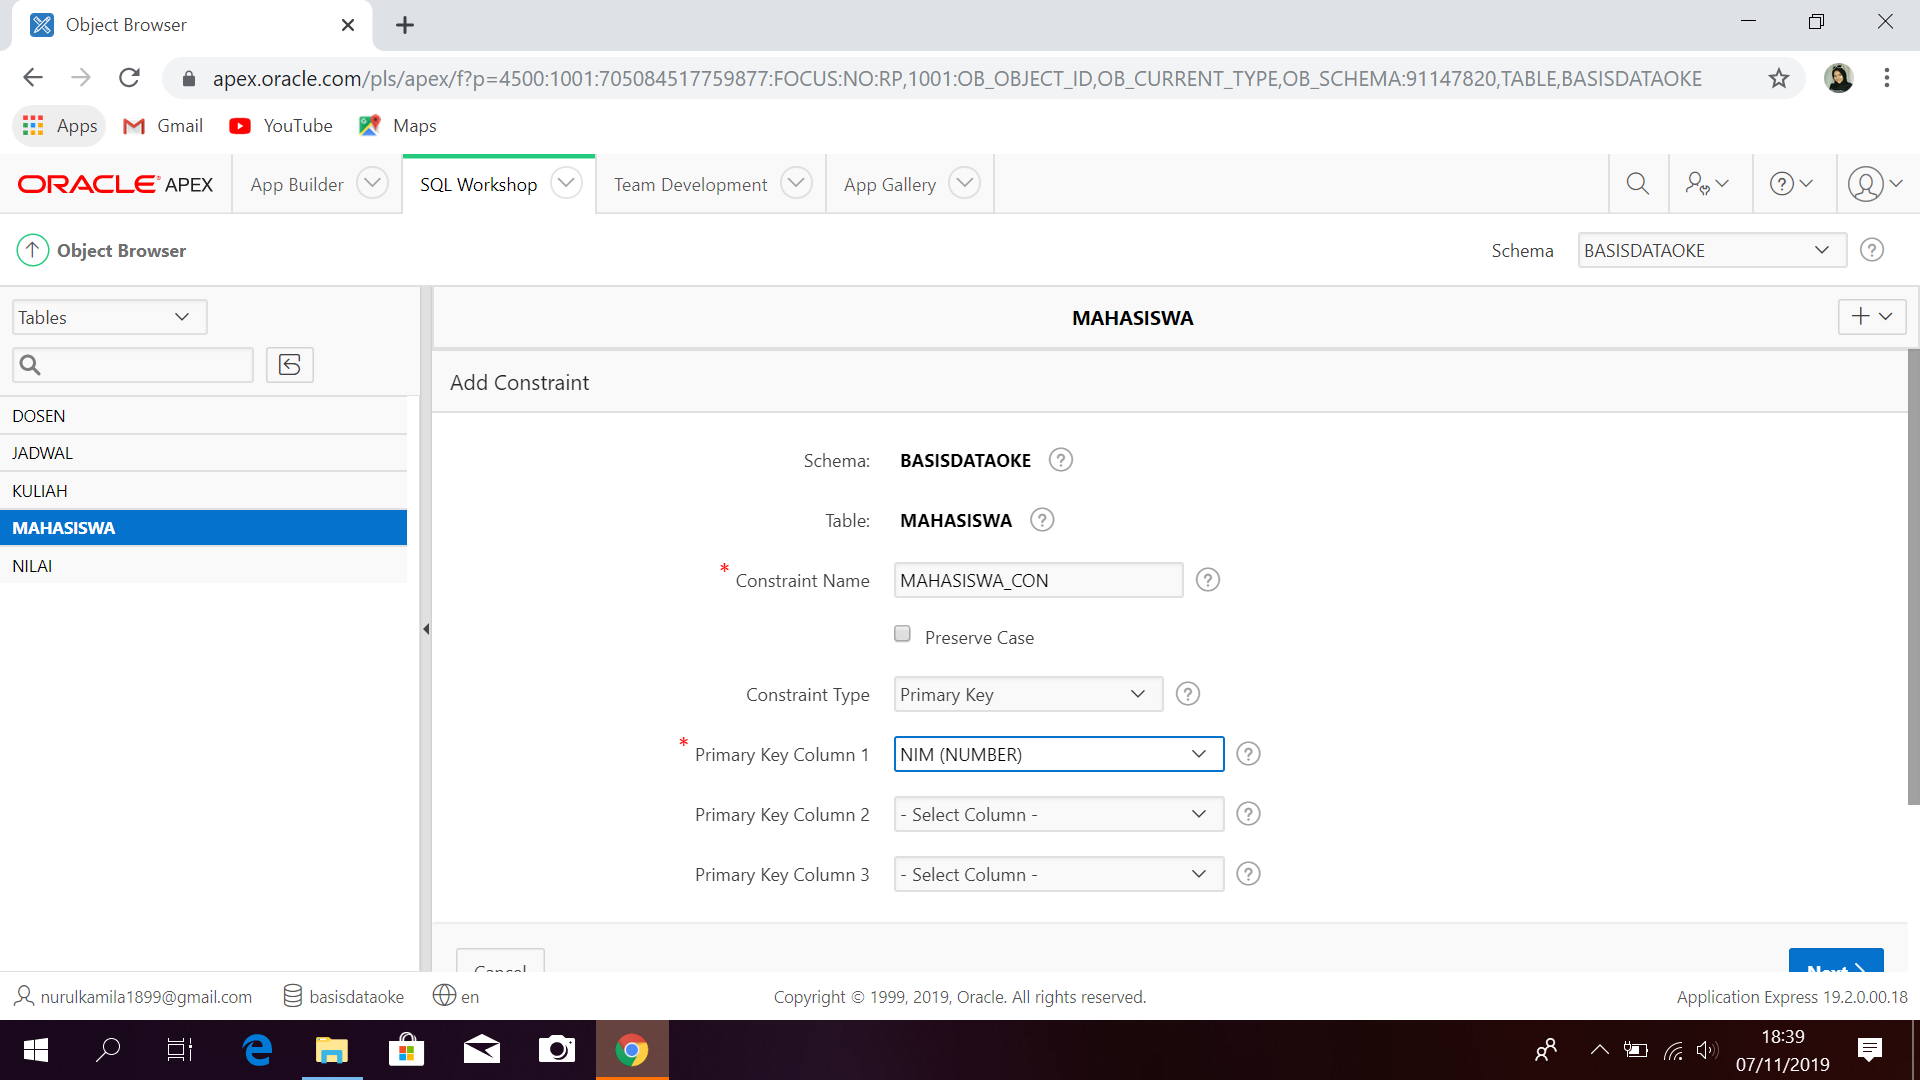
\includegraphics[width=.8\textwidth]{figure/31.PNG}
    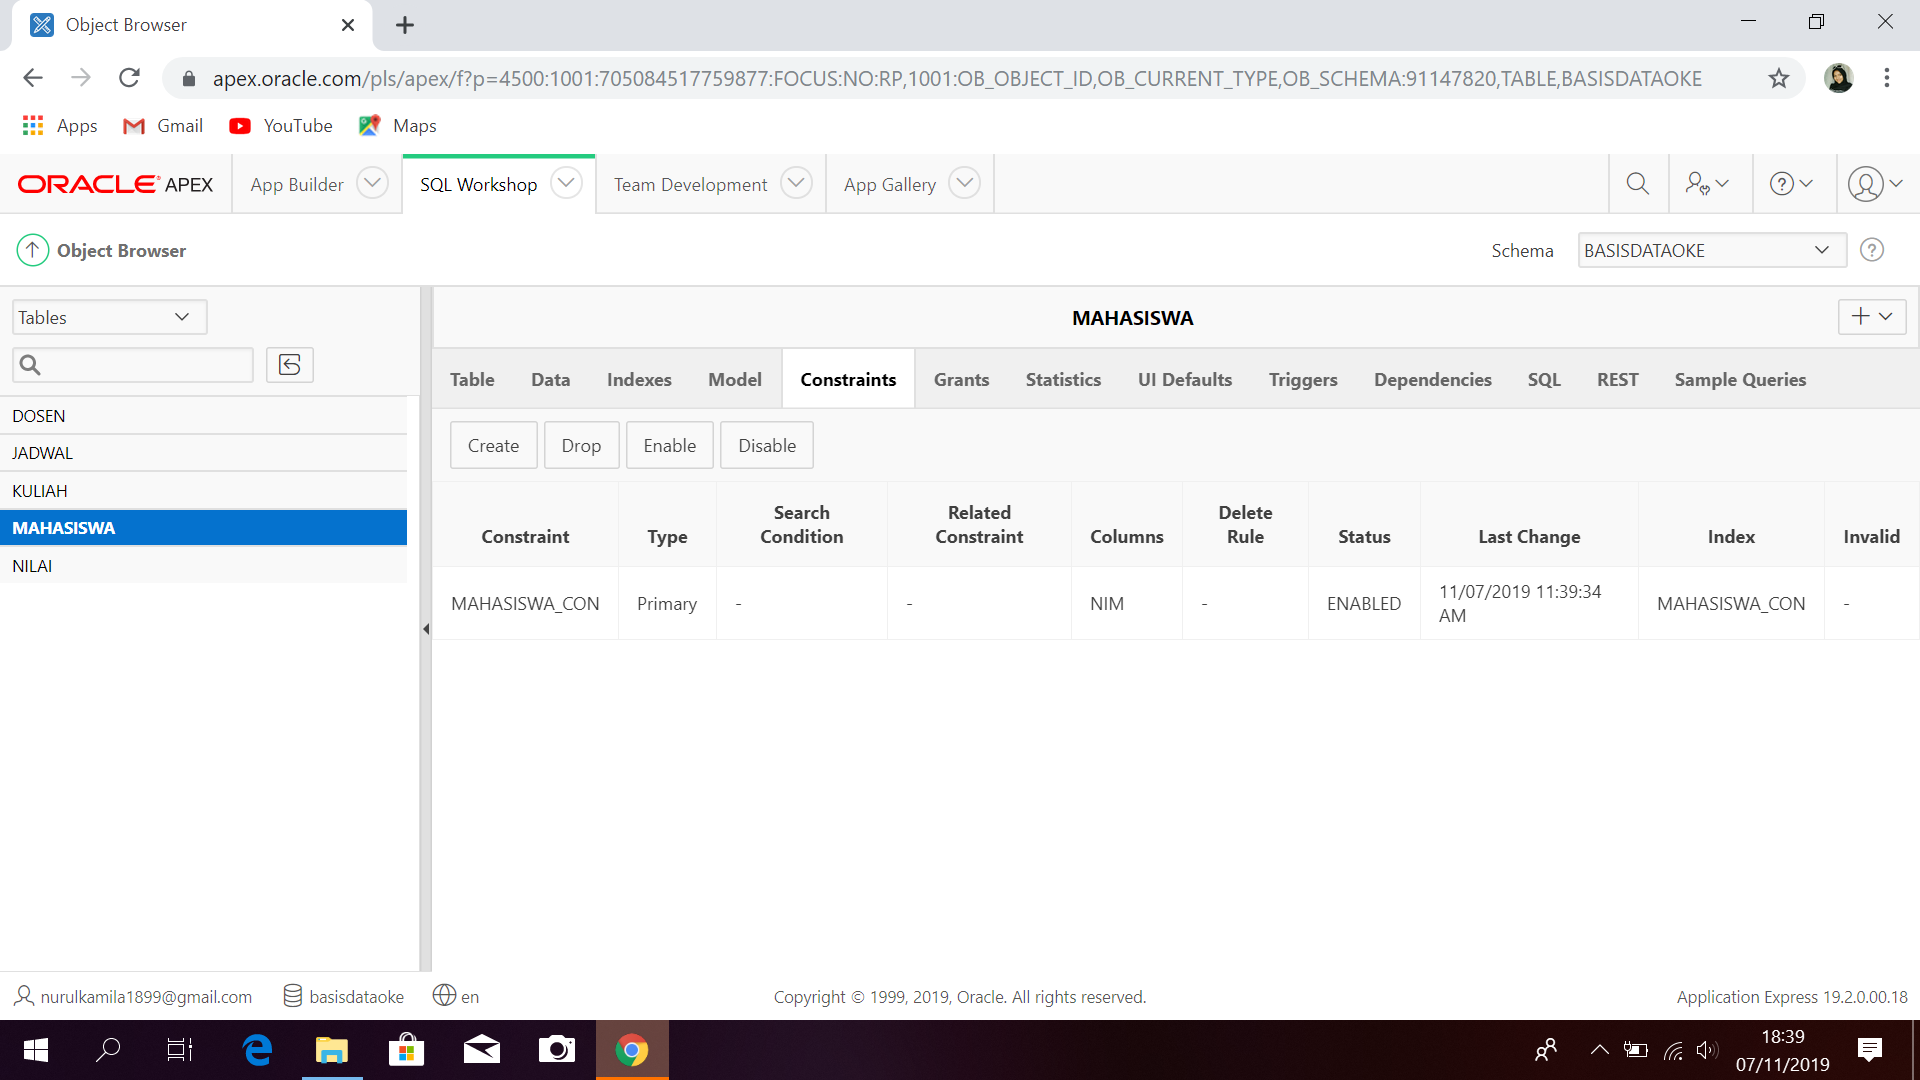
\includegraphics[width=.8\textwidth]{figure/32.PNG}
    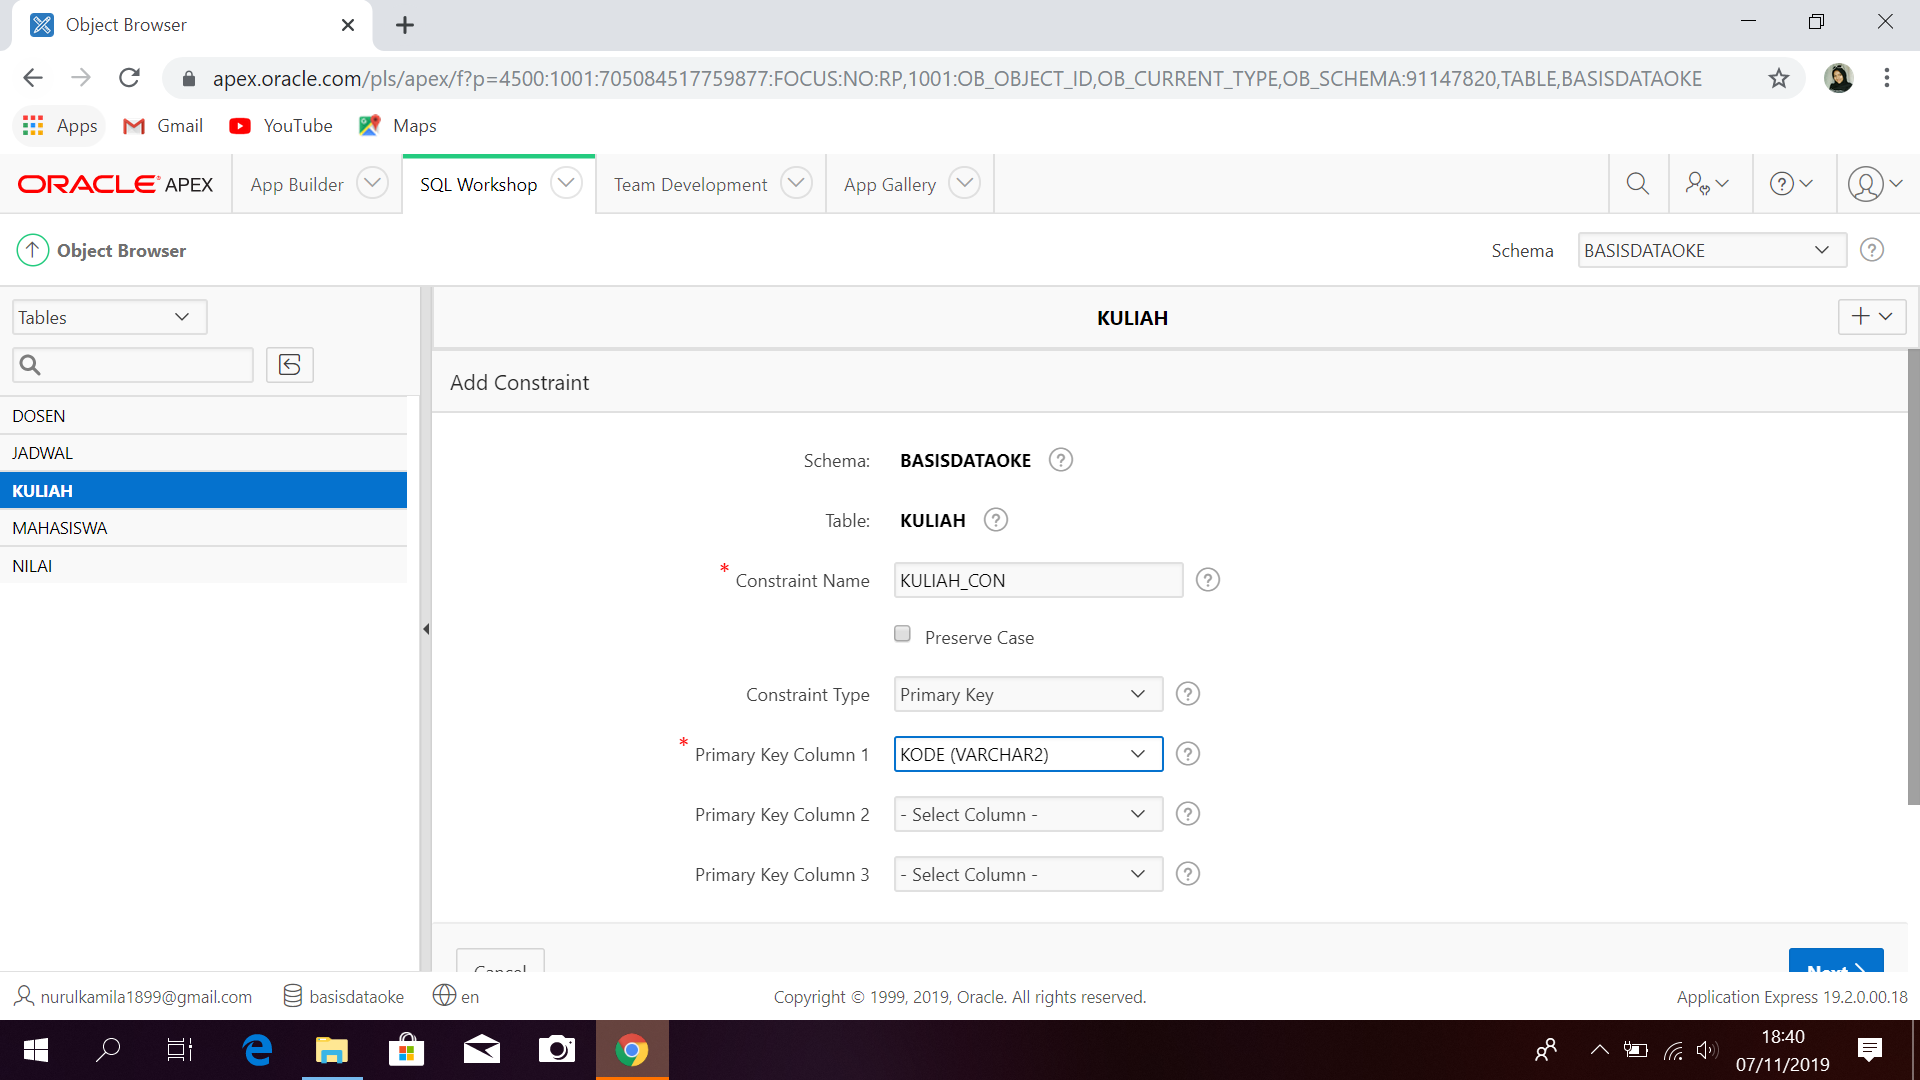
\includegraphics[width=.8\textwidth]{figure/33.PNG}
    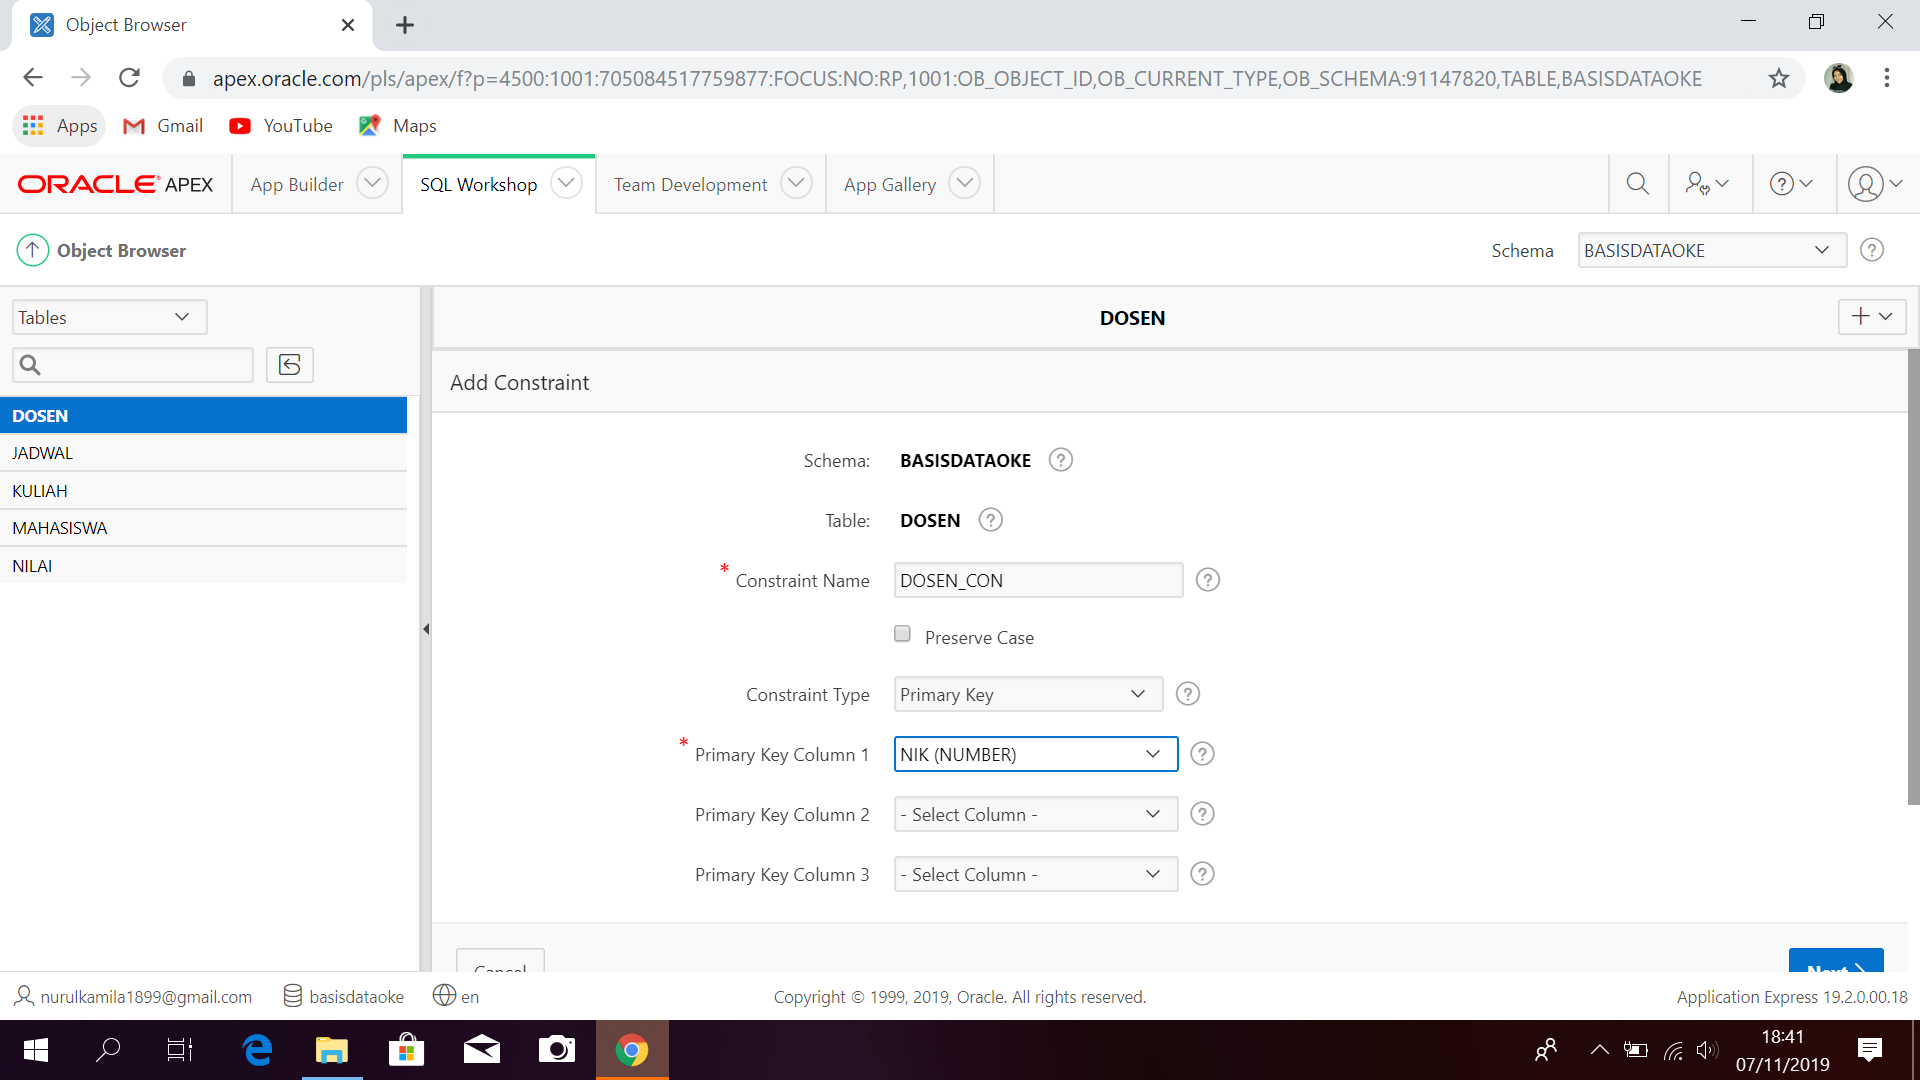
\includegraphics[width=.8\textwidth]{figure/34.PNG}
    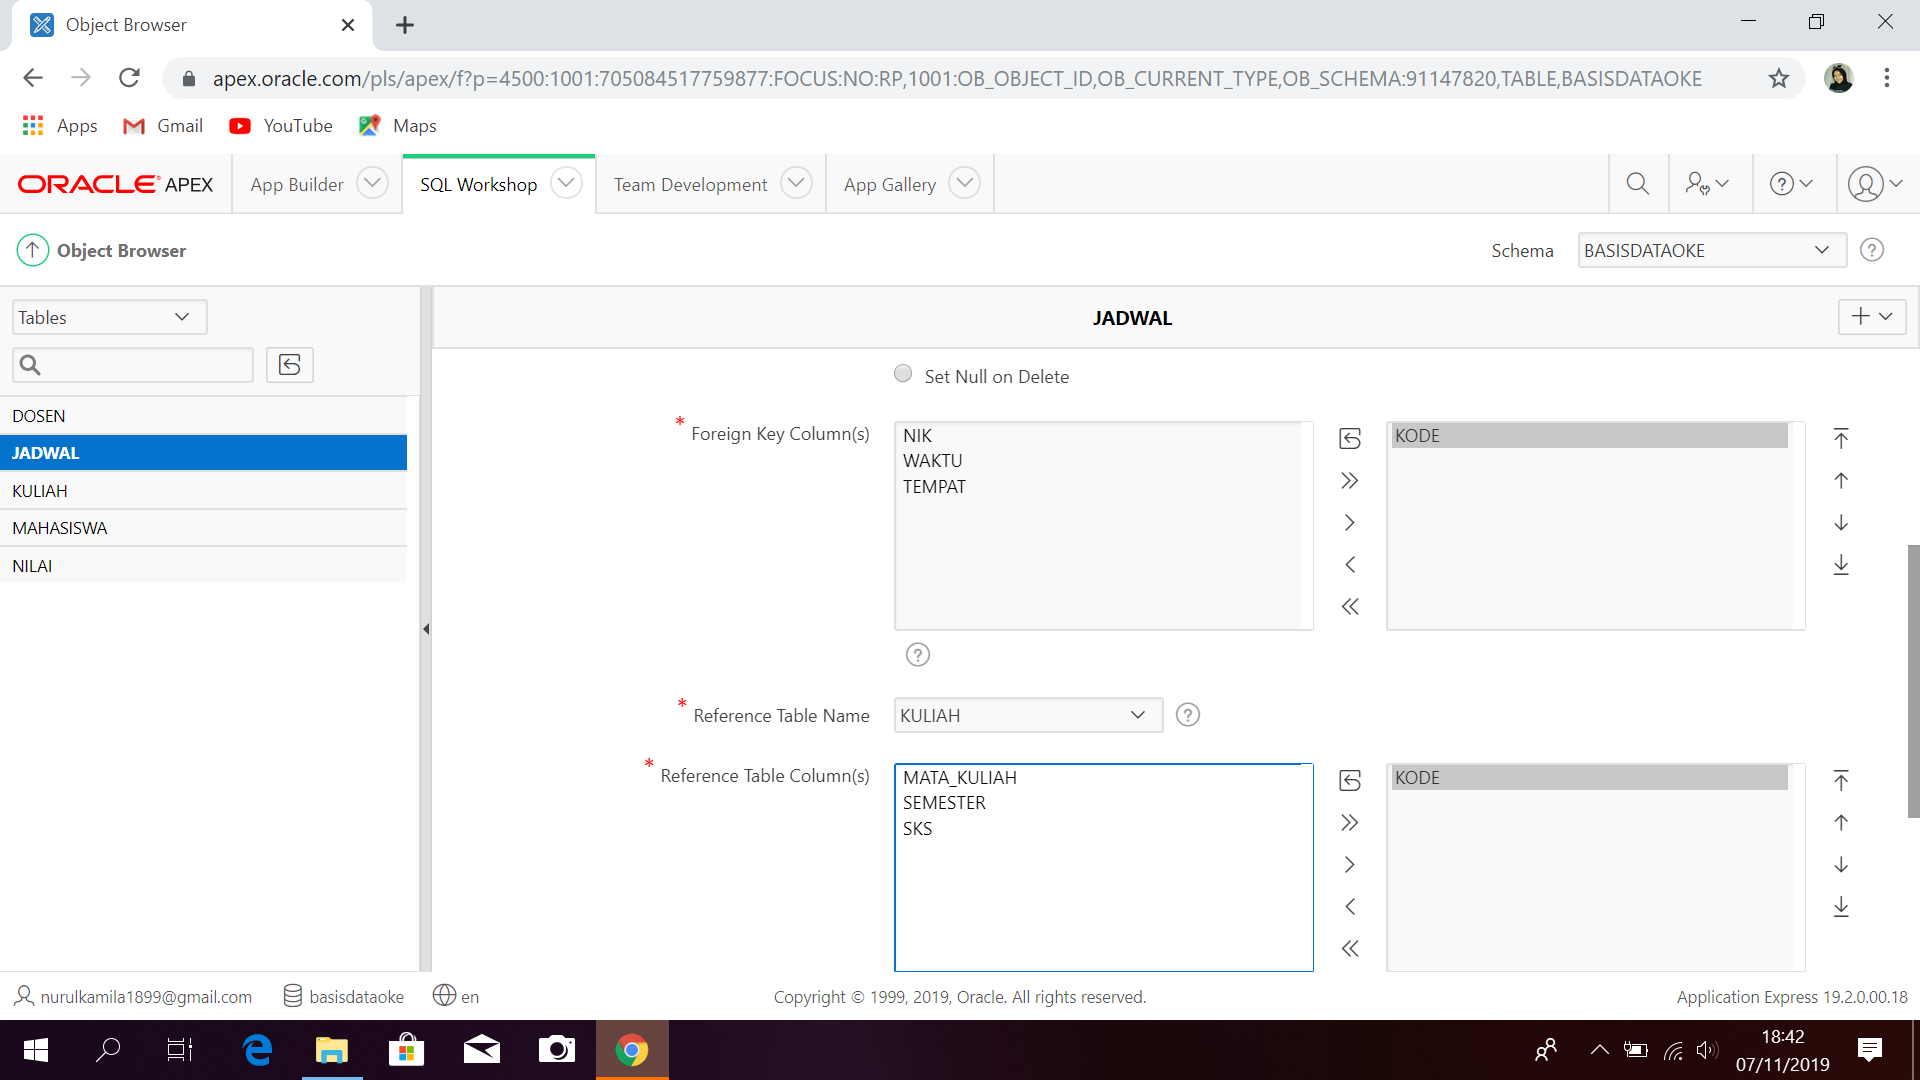
\includegraphics[width=.8\textwidth]{figure/35.PNG}
    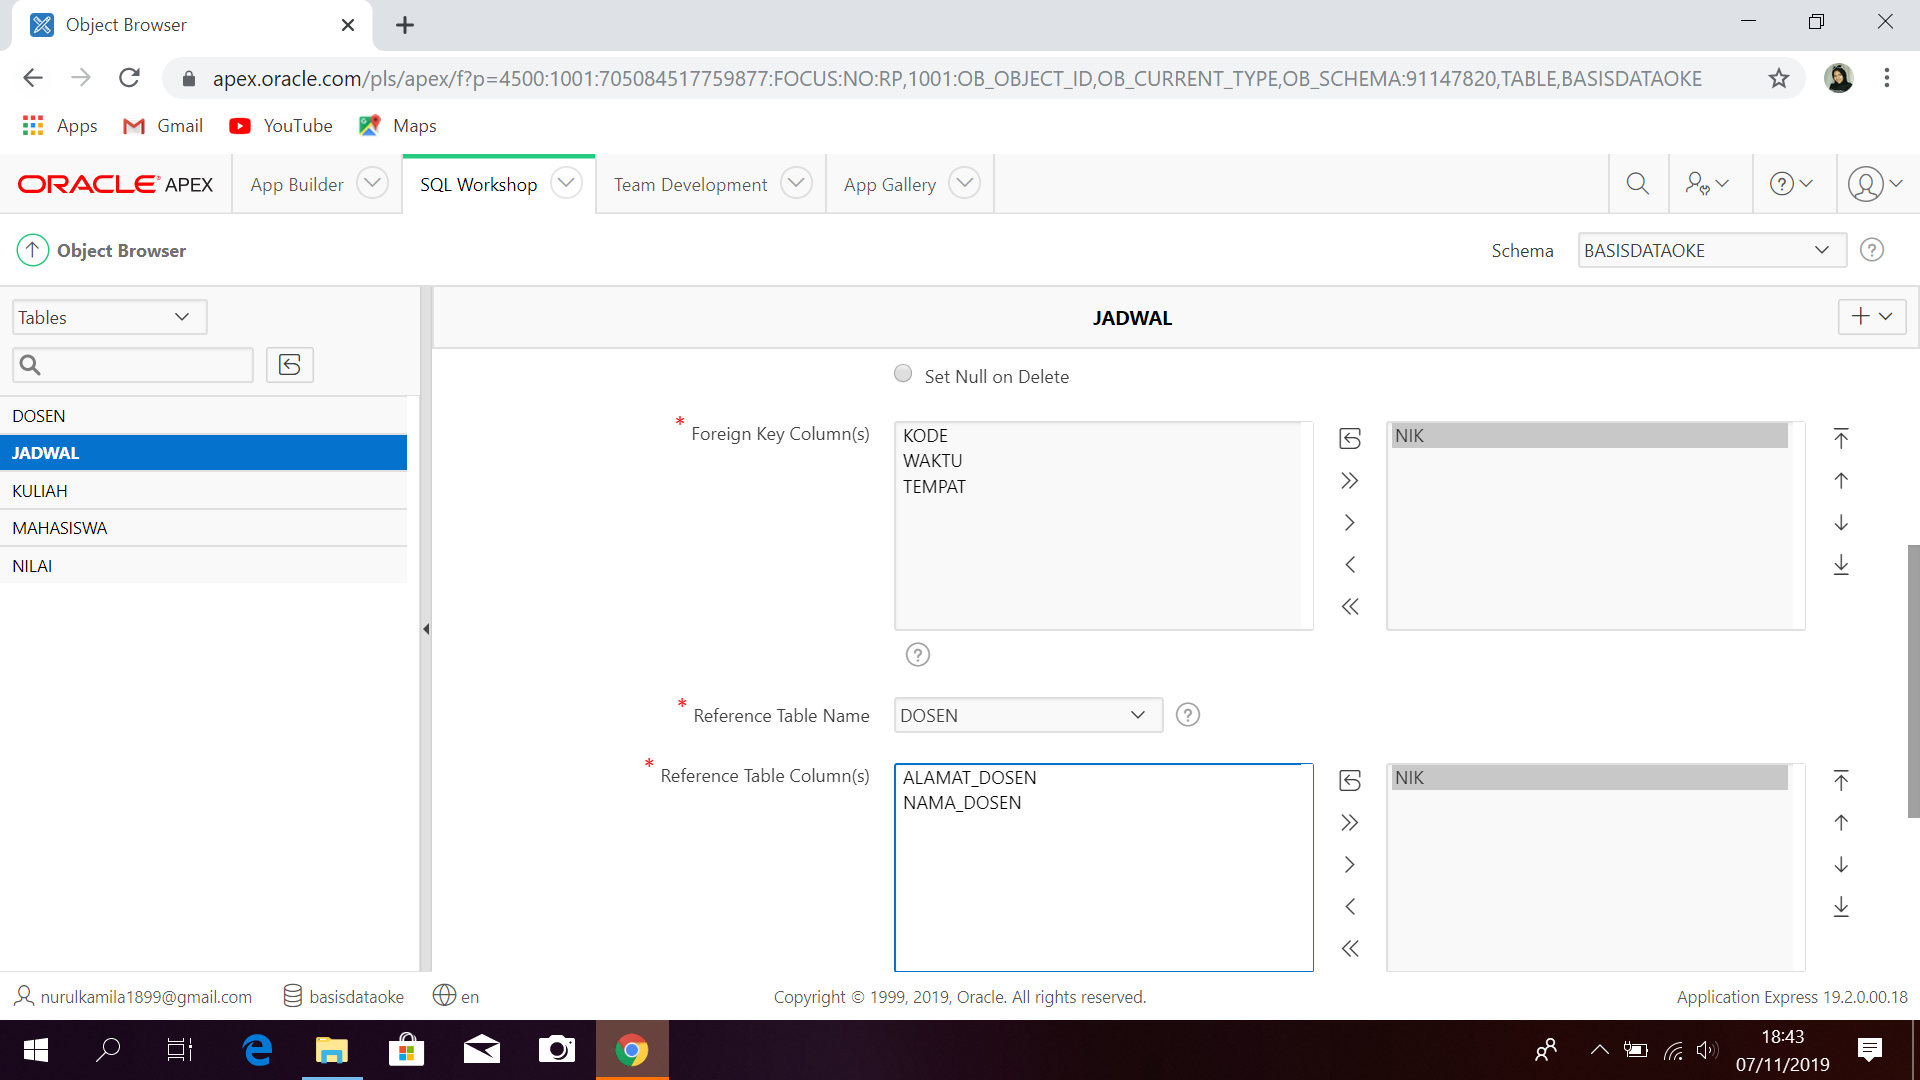
\includegraphics[width=.8\textwidth]{figure/36.PNG}
    \end{center}
    \item Lalu, kembali ke App Builder, lalu pilih New Application
     \begin{center}
    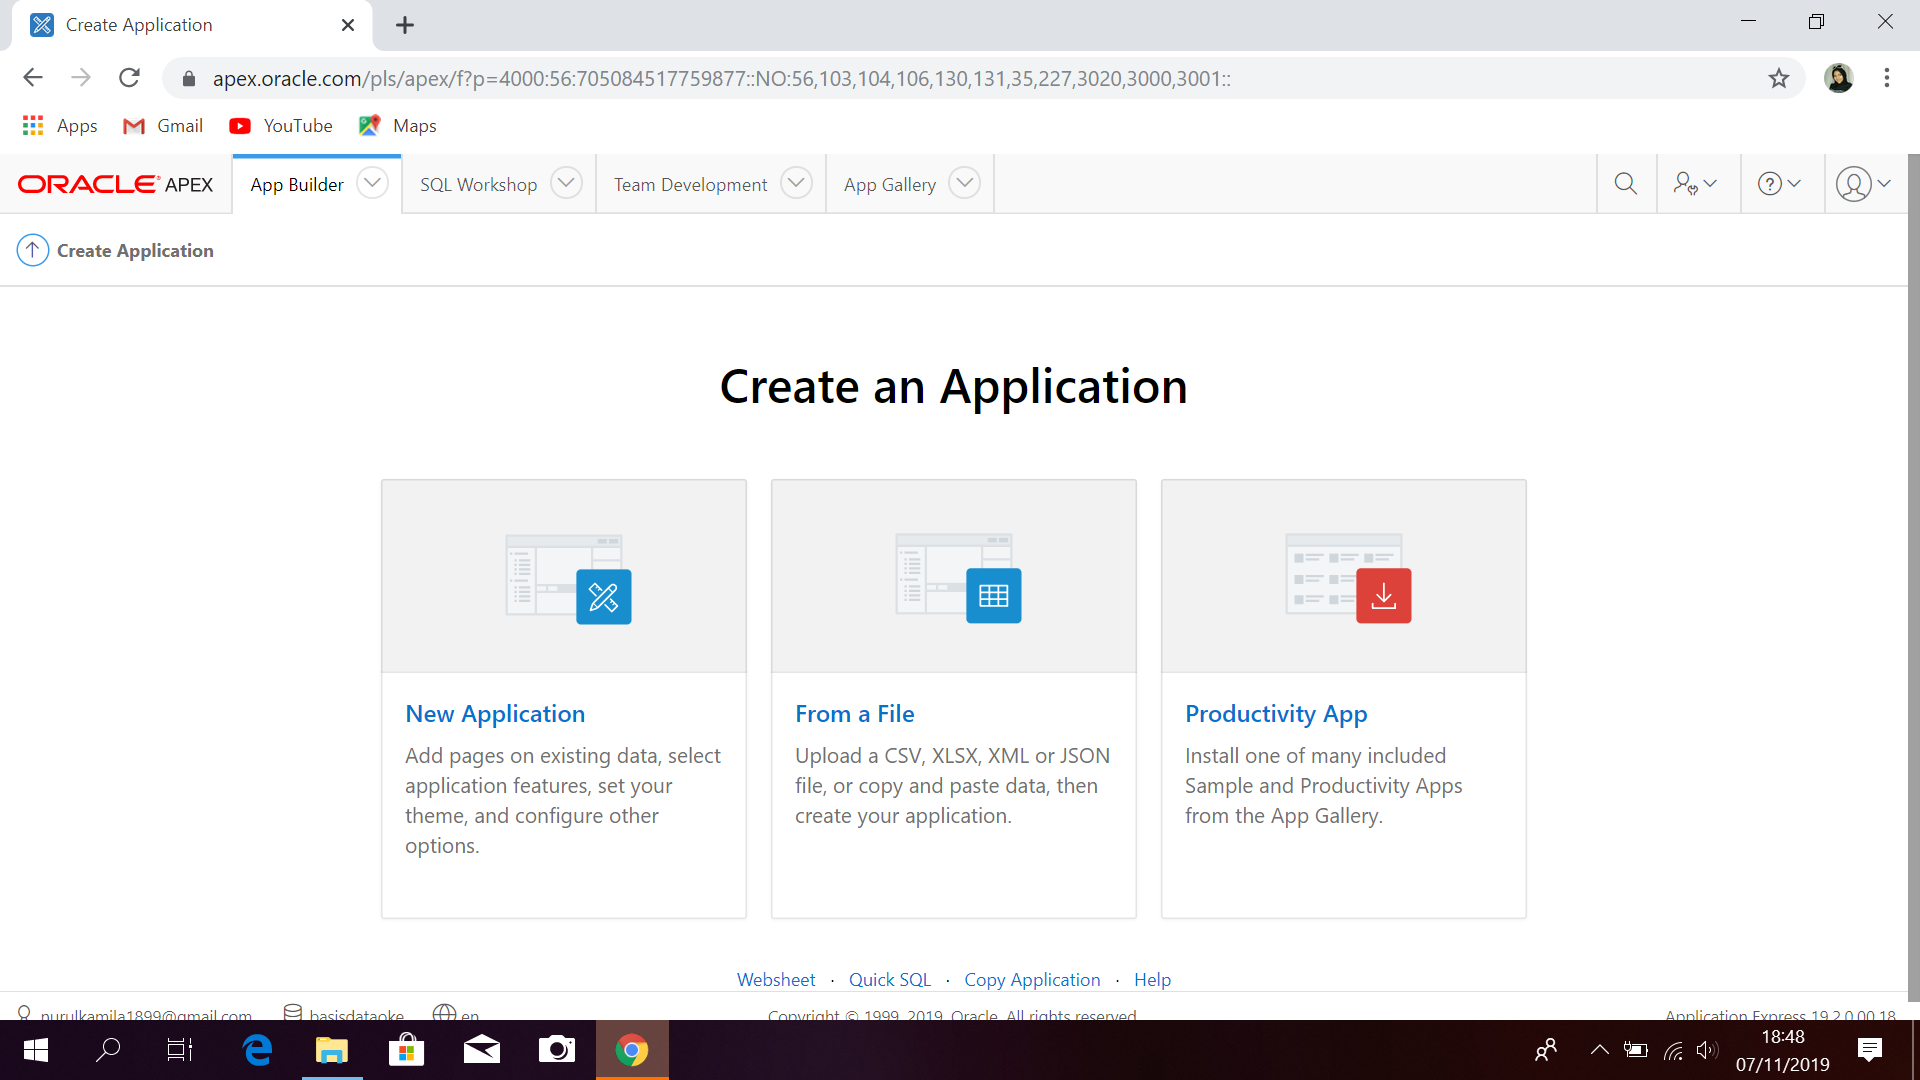
\includegraphics[width=.8\textwidth]{figure/37.PNG}
    \end{center}
    \item Add Page , lalu pilih Interactive Report
     \begin{center}
    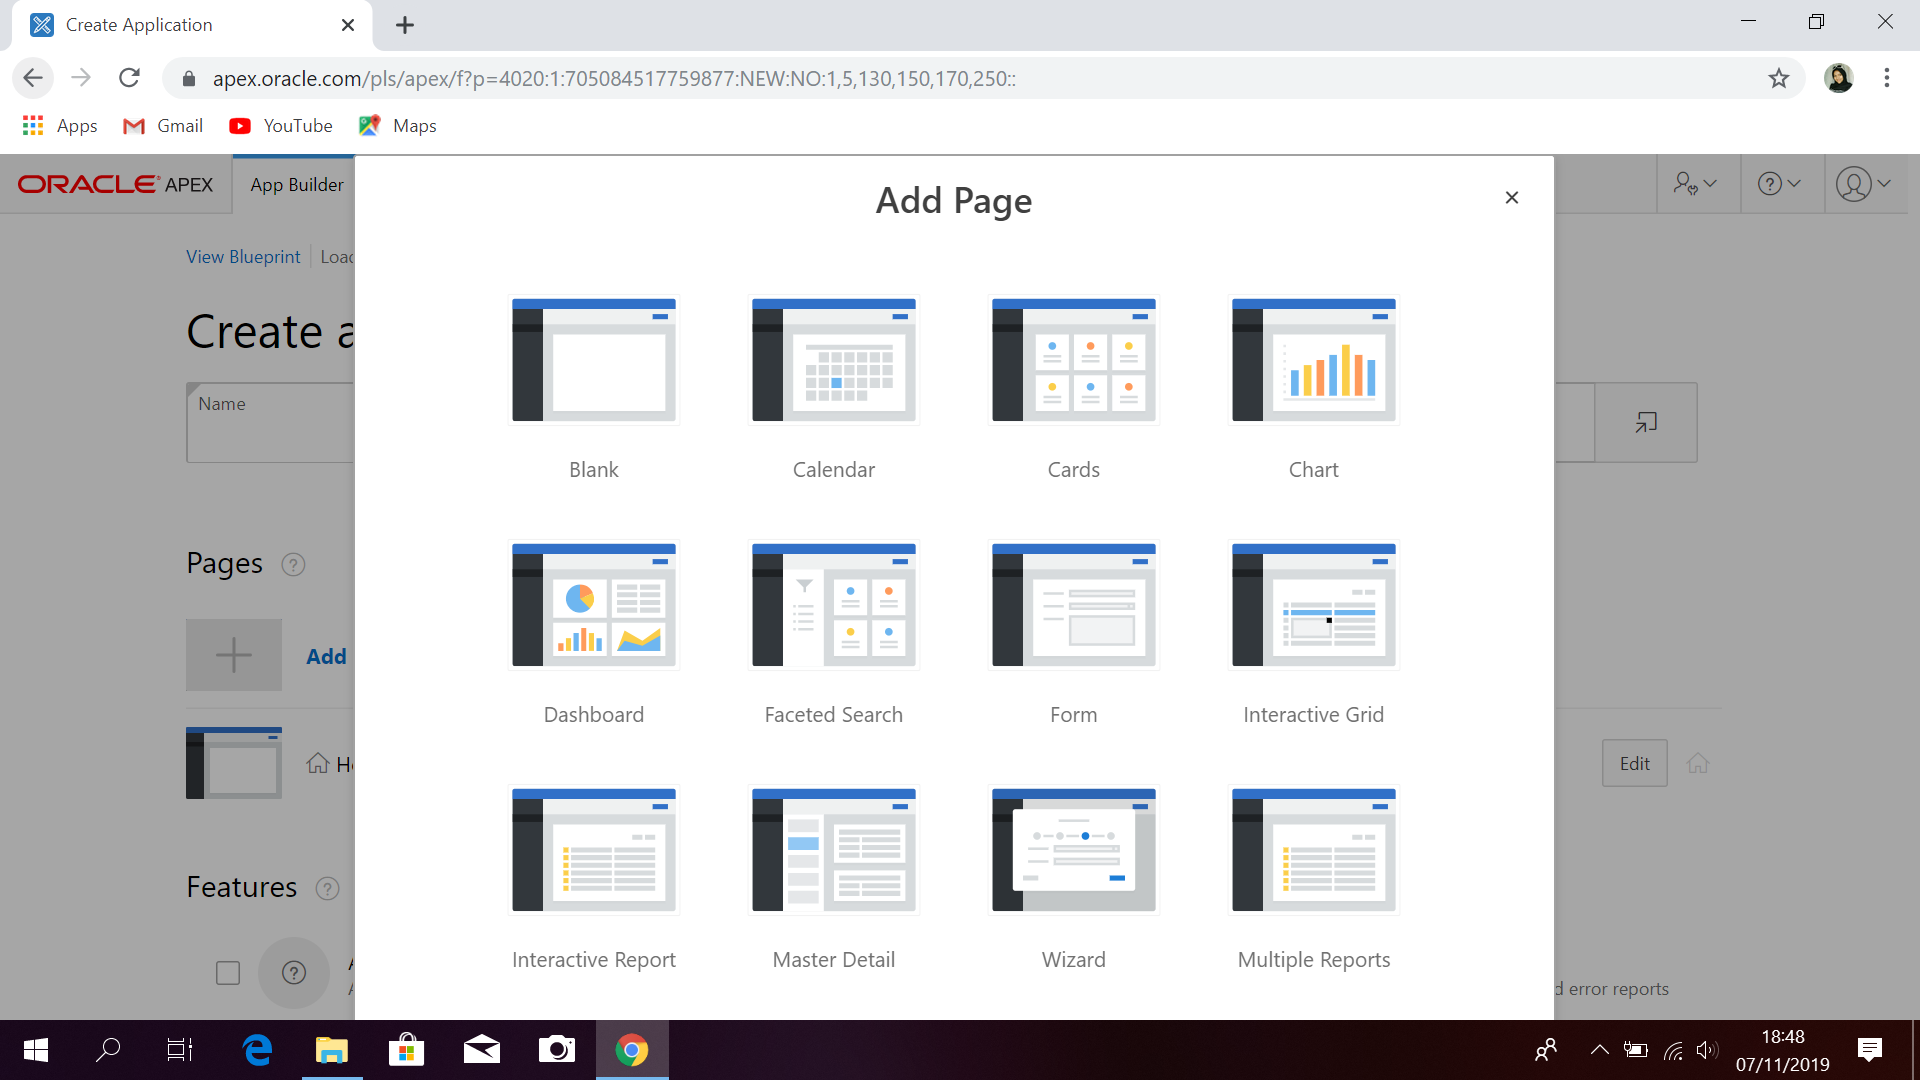
\includegraphics[width=.8\textwidth]{figure/38.PNG}
     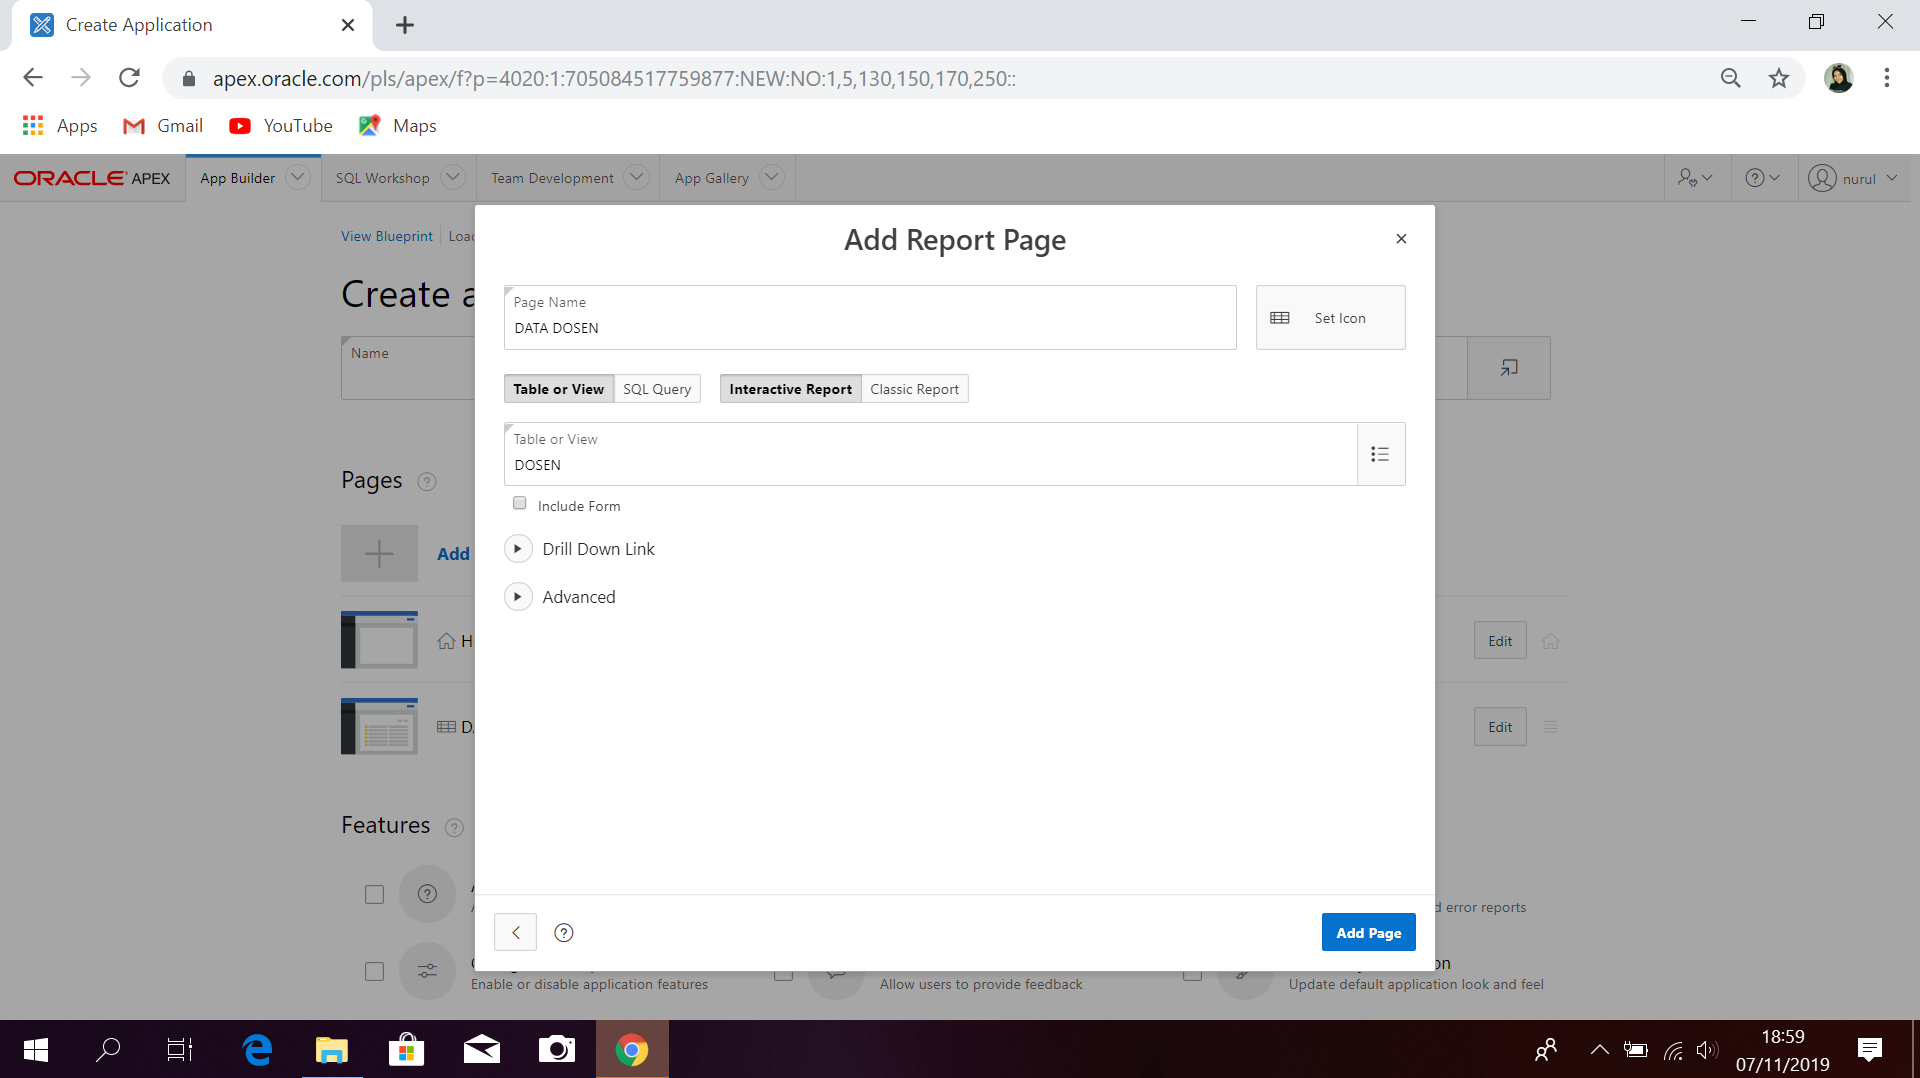
\includegraphics[width=.8\textwidth]{figure/39.PNG}
      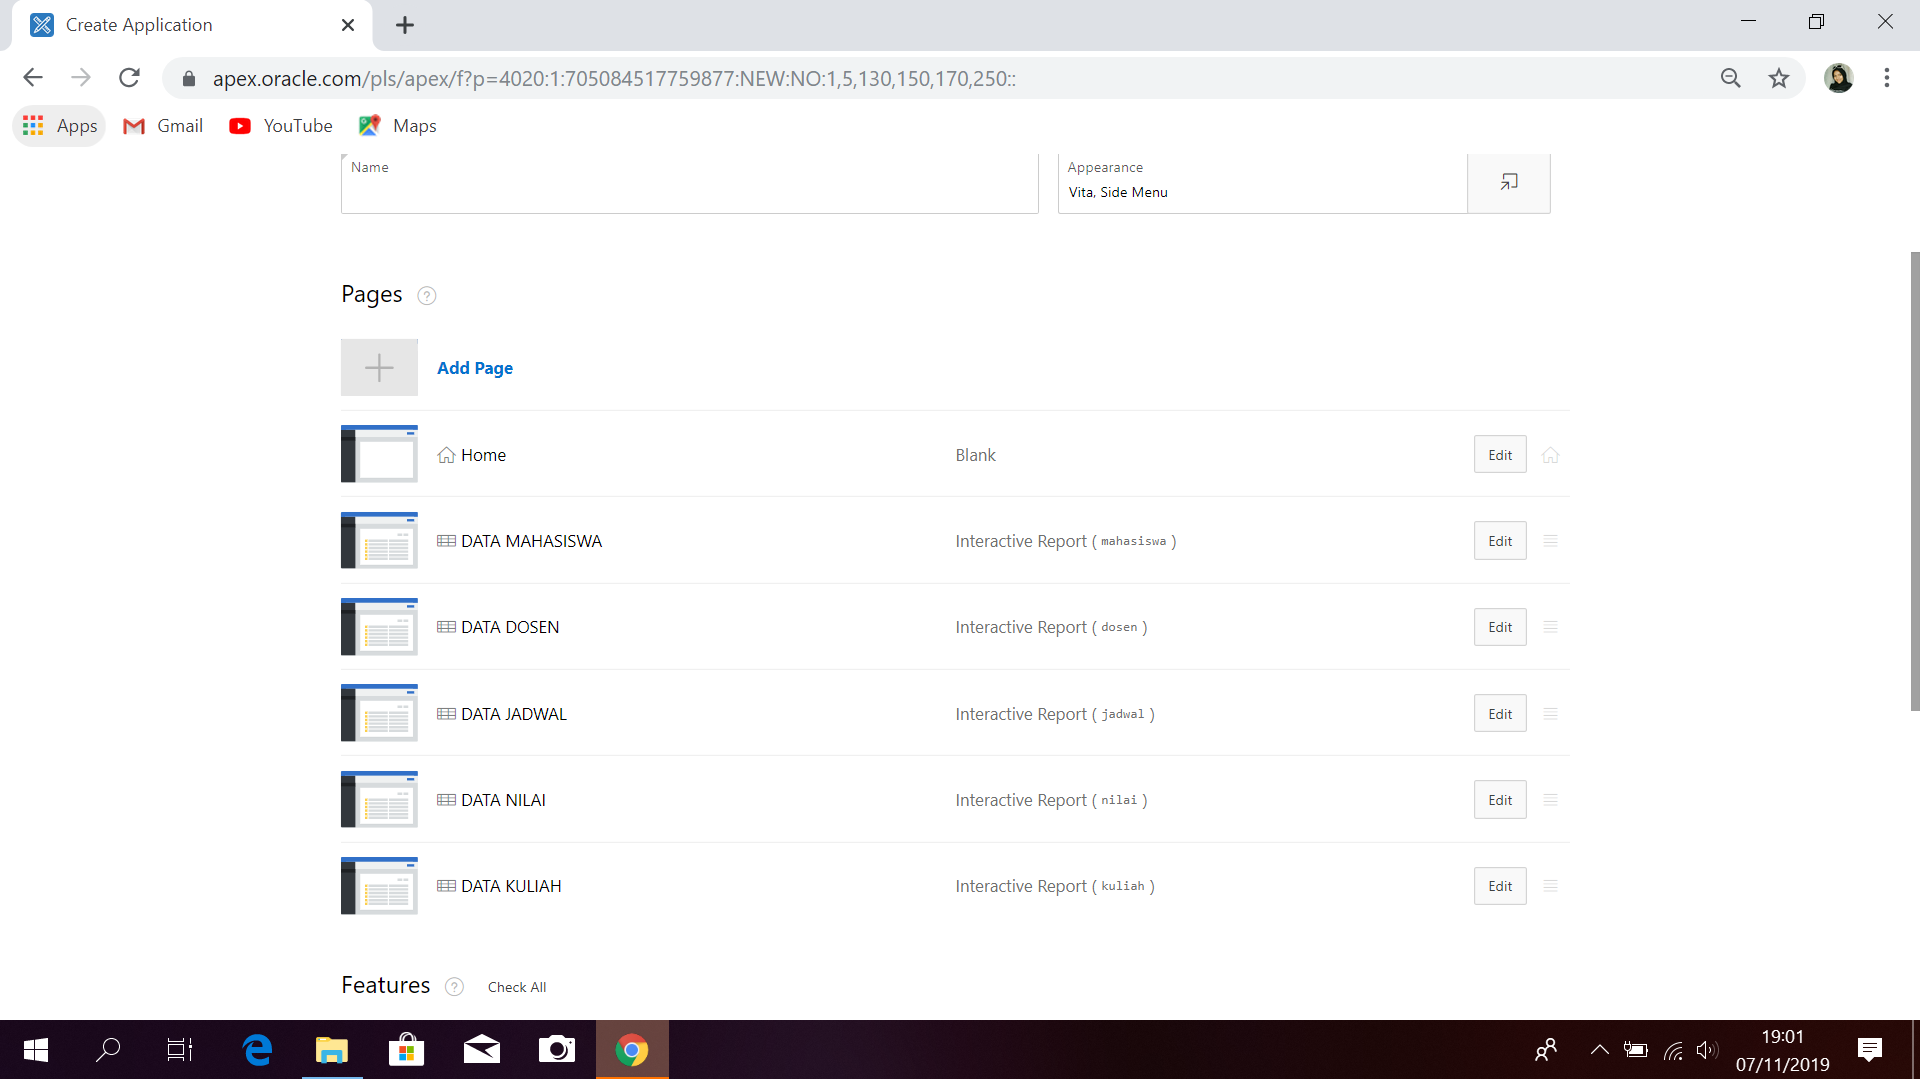
\includegraphics[width=.8\textwidth]{figure/40.PNG}
       \includegraphics[width=.8\textwidth]{figure/41.PNG}
    \end{center}
    \item jika sudah semua,kita Run Application
     \begin{center}
    \includegraphics[width=.8\textwidth]{figure/42.PNG}
    \includegraphics[width=.8\textwidth]{figure/172.png}
    \includegraphics[width=.8\textwidth]{figure/173.png}
    \end{center}
    
\end{enumerate}

\section{link login  https://apex.oracle.com/pls/apex/f?p=4000:1:6488235935386::NO:RP:FB_FLOW_ID,F4000_P1_FLOW:75957,75957 \\
Username : annisakhairani212@gmail.com \\
Password :annisa2102 }

\end{document}
